\باب{خطی الجبرا: سمتیات}
\حصہ{غیر سمتیات اور سمتیات}\شناخت{حصہ_الجبرا_سمتیات_غیر_سمتیات}
طبیعیات اور جیومیٹری میں ایسی قیمتیں پائی جاتی ہیں جنہیں ان کی مقدار سے مکمل طور پر بیان کیا جا سکتا ہے۔مثلاً  کمیت، درجہ حرارت، برقی بار، وقت، رقبہ، حجم، فاصلہ، برقی دباو وغیرہ۔ان میں سے ہر ایک کو (مقدار کی موزوں اکائی چن کر) ایک عدد  سے ظاہر کیا جا سکتا ہے۔ ایسی تمام مقداروں کو \اصطلاح{غیر سمتیات}\فرہنگ{غیر سمتیات}\فرہنگ{سمتیہ!غیر}\حاشیہب{scalars}\فرہنگ{scalars} کہتے ہیں۔غیر سمتی مقدار کی قیمت پر چننی گئی محدد کا کوئی اثر نہیں ہو گا۔

اس کے برعکس طبیعیات اور جیومیٹری میں ایسی قیمتیں بھی پائی جاتی ہیں جن کی مکمل اظہار کے لئے ان کی قیمت کے علاوہ ان کی سمت بھی درکار ہوتی ہے۔ان کی ایک مثال میکانی  قوت ہے۔ آپ جانتے ہیں کہ قوت کو تیر کی نشان سے ظاہر کیا جا سکتا ہے جہاں تیر کی سمت، قوت کی سمت اور تیر کی لمبائی (کسی پیمائش کے تحت) قوت کی مقدار کو ظاہر کرتی ہے۔ شکل \حوالہ{شکل_الجبرا_قوت_سمتی_رفتار}-الف میں ہلکے دھاگے سے بندھی ہوئی کمیت \عددی{m} کی دائری حرکت دکھائی گئی ہے۔کمیت کی لمحاتی سمتی رفتار \عددی{\bM{v}} کو تیر سے دکھایا گیا ہے۔اس تیر کی سمت، کمیت کی لمحاتی سمتی رفتار دیتی ہے جبکہ تیر کی لمبائی (کسی موزوں تناسب سے) لمحاتی سمتی رفتار کی قیمت دیتی ہے۔شکل میں کمیت کی اسراع \عددی{\bM{a}} بھی دکھائی گئی ہے جہاں \عددی{\bM{a}} کی لمبائی (کسی موزوں تناسب سے) لمحاتی اسراع کی قیمت دیتی ہے۔

سیدھی سطح میں تکون کی (بلا گھومے) منتقلی شکل \حوالہ{شکل_الجبرا_قوت_سمتی_رفتار}-ب میں  دکھائی گئی ہے۔اس حرکت کو (تکون کے ہر نقطے کی) طے فاصلے  کی مقدار اور سمت سے ظاہر کیا جا سکتا ہے۔تکون پر کسی نقطے کی ابتدائی مقام \عددی{A} سے اختتامی مقام \عددی{B} تک سمتی خط سے اس حرکت کو ظاہر کیا جا سکتا ہے۔یوں سمتی خط \عددی{\bM{b}}، تکون کے ایک نقطہ کی \عددی{A} سے \عددی{B} منتقلی دکھاتی ہے۔تکون کے ہر نقطے کی ابتدائی مقام سے اختتامی مقام تک سمتی خطوط کھینچ کر ہمیں سمتی خطوط کی نسل ملتی ہے جس میں تمام سمتی  خطوط کی لمبائی ایک جیسی  اور  سمت  ایک جیسی ہو گی (یعنی یہ آپس میں متوازی ہوں گے)۔ ہم کہہ سکتے ہیں کہ ان میں سے ہر ایک سمتی خط، تکون کے ایک نقطے کی ابتدائی مقام سے اختتامی مقام تک منتقلی کو ظاہر کرتی ہے۔ 


اس سے سمتیہ کی درج ذیل تعریف بیان کی جا سکتی ہے۔
\begin{figure}
\centering
\begin{subfigure}{0.5\textwidth}
\centering
\begin{tikzpicture}
\draw[dashed] (0,0) circle (1cm);
\draw[gray](0,0)--++(30:1cm)node[circ]{}node[right,color=black]{\RL{کمیت $m$}};
\draw[-latex](30:1cm)--++(120:0.75cm)node[above]{$\bM{v}$};
\draw[-latex](30:1cm)--++(30:-0.5cm)node[below]{$\bM{a}$};
\end{tikzpicture}
\caption*{(الف) سمتی رفتار اور اسراع۔}
\end{subfigure}%
\begin{subfigure}{0.5\textwidth}
\centering
\begin{tikzpicture}
\draw(0,0)--++(1.5,0)--++(0,1)--++(-1.5,-1);
\draw(15:3)--++(1.5,0)--++(0,1)--++(-1.5,-1);
\draw[-latex](1.5,0.25)node[ocirc]{}node[below right]{$A$}--++(15:3)node[ocirc]{}node[below right]{$B$}node[pos=0.4,below]{$\bM{b}$};
\end{tikzpicture}
\caption*{(ب) سمتیہ کی دم اور  سر۔}
\end{subfigure}%
\caption{سمتیہ کی تفصیل۔}
\label{شکل_الجبرا_قوت_سمتی_رفتار}
\end{figure}
%=================
\ابتدا{تعریف}\quad سمتیہ\\
سمتی خط کو \اصطلاح{سمتیہ}\فرہنگ{سمتیہ}\حاشیہب{vector}\فرہنگ{vector} کہتے ہیں۔اس کی لمبائی کو سمتیہ کی \اصطلاح{لمبائی} اور سمت کو سمتیہ کی \اصطلاح{سمت} کہتے ہیں۔دو سمتیات صرف اور صرف اس صورت ایک دوسرے کے برابر ہوں گے جب ان کی لمبائی ایک جیسی ہو اور ان کی سمت ایک جیسی ہو۔

سمتیہ کی لمبائی کو سمتیہ کی \اصطلاح{اقلیدسی معیار}\فرہنگ{اقلیدسی معیار}\حاشیہب{Euclidean norm}\فرہنگ{Euclidean norm} (یا معیار) اور سمتیہ کی \اصطلاح{مقدار}\فرہنگ{مقدار!سمتیہ}\فرہنگ{سمتیہ!مقدار}\حاشیہب{magnitude}\فرہنگ{magnitude} بھی کہتے ہیں۔
\انتہا{تعریف}  
%=========================

سمتیہ کی ابتدائی نقطے کو سمتیہ کی \اصطلاح{دم}\فرہنگ{دم}\فرہنگ{سمتیہ!دم}\حاشیہب{tail}\فرہنگ{tail} اور اختتامی نقطے کو سمتیہ کا \اصطلاح{سر}\فرہنگ{سر}\فرہنگ{سمتیہ!سر}\حاشیہب{head}\فرہنگ{head} کہتے ہیں۔ یوں شکل \حوالہ{شکل_الجبرا_قوت_سمتی_رفتار}-ب میں نقطہ \عددی{B} سمتیہ \عددی{\bM{b}} کی دم  ہے جبکہ نقطہ \عددی{A} اس کا سر  ہے۔

ہم سمتیات کو موٹی لکھائی میں چھوٹی حروف تہجی مثلاً \عددی{\bM{a}}، \عددی{\bM{b}}، \عددی{\bM{v}}، وغیرہ،  سے ظاہر کرتے ہیں۔ قلم و کاغذ استعمال کرتے ہوئے سمتیہ پر تیر  یا آدھے تیر کا نشان بنایا جاتا ہے یوں اسراع کو \عددیء{\vec{a}} یا  
$\overset{\rightharpoonup}{\rule{0pt}{.9ex}\smash{a}}$
لکھا جاتا ہے۔سمتیہ \عددی{\bM{a}} کی مقدار کو \عددی{\abs{\bM{a}}} لکھا جاتا ہے۔

سمتیہ کی تعریف سے ظاہر ہے کہ ہم سمتیہ کو بغیر گھمائے  ایک جگہ سے دوسری جگہ منتقل کر سکتے ہیں\حاشیہد{یہاں یہ بتلانا ضروری ہے کہ طبیعیات اور جیومیٹری میں ایسی صورتیں پائی جاتی ہیں جہاں سمتیہ  کو ایک جگہ سے دوسری  جگہ منتقل کرنا ممکن نہیں ہوتا ہے۔آپ میکانیات سے جانتے ہیں کہ کسی بھی غیر لچکدار مادے پر قوت کا اطلاق، قوت کی سمت میں لکیر پر رہتے ہوئے،  کسی بھی نقطے پر کیا جا سکتا ہے۔اس سے \اصطلاح{قابل منتقلی سمتیہ}\فرہنگ{سمتیہ!قابل منتقلی}\فرہنگ{vector!sliding} کا تصور پیدا ہوتا ہے۔اس کے برعکس، لچکدار مادے پر قوت کے اطلاق کا نقطہ تبدیل کرنے سے نتائج تبدیل ہوں گے  جو نا قابل قبول بات ہے۔یہ حقیقت \اصطلاح{مقید سمتیہ}\فرہنگ{مقید!سمتیہ}\فرہنگ{سمتیہ!مقید}\فرہنگ{bound vector}\فرہنگ{vector!bound} کی تصور کو جنم دیتی ہے۔اس کتاب میں صرف قابل منتقلی سمتیات پر بات کی جائے گی۔} یعنی ہم سمتیہ کی دم کہیں پر بھی منتقل کر سکتے ہیں۔ظاہر ہے کہ سمتیہ کی دم کا مقام مقرر کرنے سے اس کے سر کا مقام بھی مقرر ہو گا۔

اگر دو سمتیات \عددی{\bM{a}} اور \عددی{\bM{b}} ایک دوسرے کے برابر ہوں تب ہم درج ذیل لکھتے ہیں
\begin{align}
\bM{a}=\bM{b}
\end{align}
اور اگر یہ آپس میں برابر نہ ہوں تب ہم درج ذیل لکھتے ہیں۔
\begin{align}
\bM{a}\ne\bM{b}
\end{align}
کسی بھی سمتیہ کو ترسیمی طور پر موزوں  لمبائی اور سمت کی سمتی خط سے ظاہر کیا جا سکتا ہے۔

ایسا سمتیہ جس کی لمبائی اکائی \عددی{(1)} ہو \اصطلاح{اکائی سمتیہ}\فرہنگ{اکائی!سمتیہ}\فرہنگ{سمتیہ!اکائی}\حاشیہب{unit vector}\فرہنگ{vector!unit}\فرہنگ{unit!vector} کہلاتا ہے۔

%======================
\حصہ{سمتیہ کے اجزاء}
تین بُعدی فضا میں نقطہ ایک جیومیٹریائی چیز ہے جس کو محددی نظام میں تین مرتب اعداد (تصور کیا جا سکتا ہے یا) سے ظاہر  کیا جا سکتا ہے۔ گزشتہ حصے میں ہم نے سمتیہ کی تعریف جیومیٹریائی انداز میں پیش کی، جسے محددی نظام کی استعمال سے الجبرائی انداز میں بھی پیش کیا جا سکتا ہے۔

 نظام محدد  کے \اصطلاح{محور}\فرہنگ{محور}\حاشیہب{coordinates}\فرہنگ{coordinates}، آپس میں عمودی  تین متقاطع سیدھے خطوط ہوں گے۔ان کے مقام انقطاع کو محددی نظام کا \اصطلاح{مرکز}\فرہنگ{مرکز}\حاشیہب{origin}\فرہنگ{origin} کہتے ہیں۔ہم تینوں محور پر پیمائشی ناپ ایک جیسی چنتے ہیں لہٰذا   محور پر مرکز سے اکائی فاصلے پر \عددی{(1,0,0)}، \عددی{(0,1,0)} اور \عددی{(0,0,1)} نقطے پائے جائیں گے۔اس محددی نظام  کو فضا میں \اصطلاح{کارتیسی نظام محدد}\فرہنگ{کارتیسی نظام محدد}\حاشیہب{Cartesian coordinate system}\فرہنگ{Cartesian coordinate system} (شکل \حوالہ{شکل_الجبرا_کارتیسی_محدد} سے رجوع کریں) کہتے ہیں۔
\begin{figure}
\centering
\begin{tikzpicture}[x={(-0.5cm,-0.5cm)},y={(1cm,0)},z={(0,1cm)}]
\draw[-stealth](0,0,0)--++(2,0,0)node[below left]{$x$};
\draw[-stealth](0,0,0)--++(0,2,0)node[right]{$y$};
\draw[-stealth](0,0,0)--++(0,0,2)node[left]{$z$};
%
\draw(1,0,0)++(0,0.05,0)--++(0,-0.1,0)node[left]{$1$};
\draw(0,1,0)++(0,0,0.05)--++(0,0,-0.1)node[below]{$1$};
\draw(0,0,1)++(0,0.05,0)--++(0,-0.1,0)node[left]{$1$};
\end{tikzpicture}
\caption{کارتیسی نظام محددی}
\label{شکل_الجبرا_کارتیسی_محدد}
\end{figure}

ہم اب ابتدائی نقطہ \عددی{A} سے اختتامی نقطہ \عددی{B} تک سمتیہ \عددی{\bM{a}} پر غور کرتے ہیں (شکل \حوالہ{شکل_الجبرا_اجزائے_سمتیہ}-الف)۔اگر نقطہ \عددی{A} کے محور \عددی{(x_1,y_1,z_1)} اور نقطہ \عددی{B} کے محور \عددی{(x_2,y_2,z_2)} ہوں تب درج ذیل اعداد، اس کارتیسی محددی نظام کے لحاض سے،  سمتیہ \عددی{\bM{a}} کے \اصطلاح{اجزاء}\فرہنگ{اجزاء}\حاشیہب{components}\فرہنگ{components} کہلاتے ہیں۔
\begin{align}\label{مساوات_الجبرا_اجزاء_سمتیہ}
a_1=x_2-x_1,\quad a_2=y_2-y_1,\quad a_3=z_2-z_1
\end{align}
%
\begin{figure}
\centering
\begin{subfigure}{0.5\textwidth}
\centering
%axis
\begin{tikzpicture}[x={(-0.5cm,-0.5cm)},y={(1cm,0)},z={(0,1cm)}]
\draw[-stealth](0,0,0)--++(2,0,0)node[below left]{$x$};
\draw[-stealth](0,0,0)--++(0,2.5,0)node[right]{$y$};
\draw[-stealth](0,0,0)--++(0,0,2.5)node[left]{$z$};
%perpendicular drops
\draw[dashed](1,1,0.75)--(1,1,0)--(0,1,0);
\draw[dashed](1,1,0)--(1,0,0);
\draw[dashed](1.5,2,2)--(1.5,2,0)--(0,2,0);
\draw[dashed](1.5,2,0)--(1.5,0,0);
\draw[dashed](1,1,0.75)--(0,0,0.75);
\draw[dashed](1.5,2,2)--(0,0,2);
%vector
\draw[-latex,thick] (1,1,0.75)node[ocirc]{}node[shift={(0,0,0.35)}]{$A$}--(1.5,2,2)node[ocirc]{}node[right]{$B$}node[pos=0.8,left]{$\bM{a}$};
%segments
\draw[thick](1,0,0)--(1.5,0,0)node[pos=0.2,left]{$a_1$};
\draw[thick](0,1,0)--(0,2,0)node[pos=0.7,above]{$a_2$};
\draw[thick](0,0,0.75)--(0,0,2)node[pos=0.5,left]{$a_3$};
\end{tikzpicture}
\caption*{(الف) اجزائے سمتیہ}
\end{subfigure}%
\begin{subfigure}{0.5\textwidth}
\centering
%axis
\begin{tikzpicture}[x={(-0.5cm,-0.5cm)},y={(1cm,0)},z={(0,1cm)}]
\pgfmathsetmacro{\a}{1.5}
\pgfmathsetmacro{\b}{1.5}
\pgfmathsetmacro{\c}{2}
%axis
\draw[](0,0,0)--++(2,0,0);
\draw[](0,0,0)--++(0,2.5,0);
\draw[](0,0,0)--++(0,0,2.5);
%perpendicular drops
\draw[dashed](\a,\b,\c)--(\a,\b,0)--(0,\b,0);
\draw[dashed](\a,\b,0)--(\a,0,0);
\draw[dashed](\a,\b,\c)--(0,0,\c);
%segments
\draw[thick](0,0,0)--(\a,0,0)node[pos=0.2,left]{$x$};
\draw[thick](0,0,0)--(0,\b,0)node[pos=0.7,above]{$y$};
\draw[thick](0,0,0)--(0,0,\c)node[pos=0.5,left]{$z$};
%vector
\draw[-latex,thick] (0,0,0)node[ocirc]{}--(\a,\b,\c)node[ocirc]{}node[right]{$N$}node[pos=0.8,left]{$\bM{r}$};
\end{tikzpicture}
\caption*{(ب) تعین گر سمتیہ کے سر کے محور اس سمتیہ کے اجزاء ہوں گے۔}
\end{subfigure}%
\caption{سمتیہ کے اجزاء اور تعین گر سمتیہ۔}
\label{شکل_الجبرا_اجزائے_سمتیہ}
\end{figure}
سمتیہ کی تعریف کے تحت \عددی{\bM{a}} کی لمبائی سے مراد \عددی{A} سے \عددی{B} تک کی لمبائی \عددی{\overline{AB}} ہے جو مساوات \حوالہ{مساوات_الجبرا_اجزاء_سمتیہ} میں دیے گئے اجزاء کو استعمال کرتے ہوئے مسئلہ فیثاغورث کے تحت درج ذیل ہو گا۔
\begin{align}
\abs{\bM{a}}=\sqrt{a_1^2+a_2^2+a_3^2}
\end{align} 
%==============================
\ابتدا{مثال}\quad سمتیہ کے اجزاء اور اس کی لمبائی\\
سمتیہ \عددی{\bM{a}} کی دم \عددی{(-2,3,1)} اور سر \عددی{(5,-2,7)} ہیں۔اس سمتیہ کے اجزاء حاصل کرتے ہوئے سمتیہ کی لمبائی دریافت کریں۔

حل:اجزاء 
$a_1=5-(-2)=7,\quad a_2=-2-3=-5,\quad a_3=7-1=6$
اور لمبائی
\begin{align*}
\abs{\bM{a}}=\sqrt{7^2+(-5)^2+6^2}=\sqrt{110}
\end{align*}
ہے۔اگر ہم سمتیہ \عددی{\bM{a}} کی دم کو نقطہ \عددی{(4,1,3)} پر منتقل کریں تب اس کا سر \عددی{(11,-4,9)} پر ہو گا۔

مساوات \حوالہ{مساوات_الجبرا_اجزاء_سمتیہ} میں دیے گئے اجزاء کو ذہن میں رکھتے ہوئے آپ دیکھ سکتے ہیں کہ اگر \عددی{\bM{a}} کی دم کو کارتیسی محدد کی مرکز پر منتقل کیا جائے تب \عددی{\bM{a}} کے اجزاء اس کی سر کے محور ہوں گے۔ایسا سمتیہ جس کو شکل \حوالہ{شکل_الجبرا_اجزائے_سمتیہ}-ب میں دکھایا گیا ہے  \اصطلاح{تعین گر سمتیہ}\فرہنگ{تعین گر سمتیہ}\فرہنگ{سمتیہ!تعین گر}\حاشیہب{position vector}\فرہنگ{position vector}\فرہنگ{vector!position} کہلاتا ہے اور اس کو \عددی{\bM{r}} سے ظاہر کیا جاتا ہے۔ 
\انتہا{مثال}
%================================

\عددی{\bM{a}} کی دم کو ایک جگہ سے دوسری جگہ منتقل کرنے سے سمتیہ کا سر بھی اتنا ہی اپنی جگہ سے ہلتا ہے لہٰذا مساوات \حوالہ{مساوات_الجبرا_اجزاء_سمتیہ} سے ظاہر ہے کہ سمتیہ \عددی{\bM{a}} کے اجزاء \عددی{a_1}، \عددی{a_2} اور \عددی{a_3} کی قیمت پر \عددی{\bM{a}} کی ابتدائی نقطے کا کوئی اثر نہیں ہو گا۔یوں کسی بھی معین کارتیسی محددی نظام کے حوالے سے سمتیہ کو مکمل طور پر تین (محوری) اعداد سے ظاہر کیا جا سکتا ہے۔

 وہ سمتیہ  جس کے اجزاء \عددی{0}، \عددی{0}، \عددی{0} ہوں \ترچھا{معدوم سمتیہ}\فرہنگ{معدوم سمتیہ}\حاشیہب{null vector}\فرہنگ{null vector} یا \اصطلاح{صفر سمتیہ}\فرہنگ{صفر سمتیہ}\فرہنگ{سمتیہ!صفر}\حاشیہب{zero vector}\فرہنگ{vector!zero}\فرہنگ{zero!vector} \عددی{\bM{0}} کہلاتا ہے۔ یوں کوئی بھی تین اعداد بہ شمول  \عددی{0}، \عددی{0}، \عددی{0} سمتیہ کے اجزاء ہو سکتے ہیں۔

معین نظام محدد کی صورت میں  ہر مرتب تین اعداد ایک منفرد سمتیہ کو ظاہر کریں گے۔یہ تین اعداد سمتیہ کے اجزاء ہوں گے۔اسی طرح معین نظام محدد میں ہر سمتیہ کے اجزاء سے سمتیہ کو تین مرتب اعداد کی صورت میں لکھا جا سکتا ہے۔گزشتہ حصہ میں سمتیہ کی تعریف جیومیٹریائی نقطہ نظر سے کی گئی۔ہم اب تین مرتب حقیقی اعداد (جو سمتیہ کے \ترچھا{اجزاء} کہلاتے ہیں) کو سمتیہ کی \ترچھا{تعریف} کہہ سکتے ہیں۔اس تعریف کو  استعمال کرتے ہوئے ہم سمتیہ کی جیومیٹریائی صورت حاصل کر سکتے ہیں۔  

یوں دو سمتیات \عددی{\bM{a}} اور \عددی{\bM{b}} صرف اور صرف اس صورت ایک جیسے ہوں گے جب ان کے تین مطابقتی اجزاء ایک جیسے ہوں۔لہٰذا درج ذیل سمتی مساوات
\begin{align*}
\bM{a}=\bM{b}
\end{align*}
سے مراد درج ذیل تین مساوات ہیں جہاں \عددی{a_1}،\عددی{a_2}،\عددی{a_3} اور \عددی{b_1}، \عددی{b_2}، \عددی{b_3} ایک ہی کارتیسی نظام محدد میں بالترتیب \عددی{\bM{a}} اور \عددی{\bM{b}} کے مطابقتی اجزاء ہیں۔
\begin{align*}
a_1=b_1,\quad a_2=b_2,\quad a_3=b_3
\end{align*}

ظاہر ہے کہ اگر ایک سمتیہ کوئی حقیقی یا جیومیٹریائی چیز ہو تب اس کی لمبائی اور سمت پر چننی گئی نظام محدد کا کوئی اثر نہیں ہونا چاہیے۔ 

اگلے باب میں سمتیہ کے تصور کو وسعت دیتے ہوئے ہر مرتب \عددی{n} اعداد کو سمتیہ تصور کیا جائے گا، جہاں \عددی{n}  کوئی بھی مثبت عدد صحیح ہو سکتا ہے۔
%==================

\حصہء{سوالات}
سوال \حوالہ{سوال-الجبرا_اجزاء_الف} تا سوال \حوالہ{سوال-الجبرا_اجزاء_ب} میں سمتیہ \عددی{\bM{u}} کا ابتدائی نقطہ \عددی{A} اور اختتامی نقطہ \عددی{B} ہے۔ سمتیہ \عددی{\bM{u}} کے اجزاء حاصل کرتے ہوئے سمتیہ کی لمبائی \عددی{\abs{\bM{u}}} حاصل کریں۔\عددی{\bM{u}} کا خط کھینچیں۔

%==========
\ابتدا{سوال}\شناخت{سوال-الجبرا_اجزاء_الف}\quad
$A:(2,3,0), \quad B:(-4,6,0)$

جوابات: \عددی{u_3=0}،  \عددی{u_2=3}،\عددی{u_1=-6}، \عددی{\abs{\bM{u}}=3\sqrt{5}}
\انتہا{سوال}
%=============================
\ابتدا{سوال}\quad
$A:(5,3,1), \quad B:(1,7,2)$

جوابات: \عددی{u_3=1}،  \عددی{u_2=4}،\عددی{u_1=-4}، \عددی{\abs{\bM{u}}=\sqrt{33}}
\انتہا{سوال}
%======================
\ابتدا{سوال}\quad
$A:(1.2,-1,2.5), \quad B:(2.4,1.6,-3.2)$

جوابات: \عددی{u_3=-5.7}،  \عددی{u_2=2.6}،\عددی{u_1=1.2}، \عددی{\abs{\bM{u}}=6.38}
\انتہا{سوال}
%=============================
\ابتدا{سوال}\quad
$A:(0,0,3), \quad B:(4,0,0)$

جوابات: \عددی{u_3=-3}،  \عددی{u_2=0}،\عددی{u_1=4}، \عددی{\abs{\bM{u}}=5}
\انتہا{سوال}
%=============================
\ابتدا{سوال}\quad
$A:(3,3,3), \quad B:(1,1,1)$

جوابات: \عددی{u_3=-2}،  \عددی{u_2=-2}،\عددی{u_1=-2}، \عددی{\abs{\bM{u}}=2\sqrt{3}}
\انتہا{سوال}
%=============================
\ابتدا{سوال}\quad
$A:(1,1,1), \quad B:(3,3,3)$

جوابات: \عددی{u_3=2}،  \عددی{u_2=2}،\عددی{u_1=2}، \عددی{\abs{\bM{u}}=2\sqrt{3}}
\انتہا{سوال}
%=============================
\ابتدا{سوال}\quad
$A:(2,2,2), \quad B:(2,2,0)$

جوابات: \عددی{u_3=0}،  \عددی{u_2=0}،\عددی{u_1=0}، \عددی{\abs{\bM{u}}=0}؛ یہ صفر سمتیہ ہے۔
\انتہا{سوال}
%=============================
\ابتدا{سوال}\quad
$A:(0,7,8), \quad B:(-3,1,8)$

جوابات: \عددی{u_3=0}،  \عددی{u_2=6}،\عددی{u_1=-3}، \عددی{\abs{\bM{u}}=3\sqrt{5}}
\انتہا{سوال}
%=============================
\ابتدا{سوال}\quad
$A:(100,200,300), \quad B:(100,204,303)$

جوابات: \عددی{u_3=3}،  \عددی{u_2=4}،\عددی{u_1=0}، \عددی{\abs{\bM{u}}=5}
\انتہا{سوال}
%=============================
\ابتدا{سوال}\شناخت{سوال-الجبرا_اجزاء_ب}\quad
$A:(-5,-6,-2), \quad B:(-8,-6,-4)$

جوابات: \عددی{u_3=-2}،  \عددی{u_2=0}،\عددی{u_1=-3}، \عددی{\abs{\bM{u}}=\sqrt{13}}
\انتہا{سوال}
%=============================
سوال \حوالہ{سوال_الجبرا_ابتدائی_سے_اختتامی_الف} تا سوال \حوالہ{سوال_الجبرا_ابتدائی_سے_اختتامی_ب} میں ابتدائی نقطہ \عددی{A} اور سمتیہ کے اجزاء دیے گئے ہیں۔سمتیہ کا اختتامی نقطہ دریافت کریں۔

%=========================
\ابتدا{سوال}\شناخت{سوال_الجبرا_ابتدائی_سے_اختتامی_الف}\quad
$A:(-2,3,1); \quad 3,1,4$\\
جواب:\عددی{1,4,5}
\انتہا{سوال}
%===========================
\ابتدا{سوال}\quad
$A:(0,0,0); \quad 5,1,7$\\
جواب:\عددی{5,1,7}
\انتہا{سوال}
%===========================
\ابتدا{سوال}\quad
$A:(5,2,-6); \quad 0,0,0$\\
جواب:\عددی{5,2,-6}
\انتہا{سوال}
%===========================
\ابتدا{سوال}\quad
$A:(3,6,1); \quad -5,-7,2$\\
جواب:\عددی{-2,-1,3}
\انتہا{سوال}
%===========================
\ابتدا{سوال}\quad
$A:(4,4,4); \quad 4,4,4$\\
جواب:\عددی{8,8,8}
\انتہا{سوال}
%===========================
\ابتدا{سوال}\quad
$A:(7,7,7); \quad -7,-7,-7$\\
جواب:\عددی{0,0,0}
\انتہا{سوال}
%===========================
\ابتدا{سوال}\quad
$A:(-3,-4,-5); \quad  3,4,5$\\
جواب:\عددی{0,0,0}
\انتہا{سوال}
%===========================
\ابتدا{سوال}\quad
$A:(\frac{1}{2},\frac{2}{3},\frac{1}{3}); \quad  -\frac{3}{2},\frac{1}{3},1$\\
جواب:\عددی{-1,1,\tfrac{4}{3}}
\انتہا{سوال}
%===========================
\ابتدا{سوال}\quad
$A:(0.2,-0.1,0.5); \quad  1.1,-0.4,-0.3$\\
جواب:\عددی{1.3,-0.5,0.2}
\انتہا{سوال}
%===========================
\ابتدا{سوال}\شناخت{سوال_الجبرا_ابتدائی_سے_اختتامی_ب}\quad
$A:(11.3,-10,-15.8); \quad  12.6,9,-14$\\
جواب:\عددی{23.9,-1,-29.8}
\انتہا{سوال}
%===========================

\حصہ{سمتیات کا مجموعہ، غیر سمتی کے ساتھ ضرب}\شناخت{حصہ_الجبرا_ضرب_جمع}
چونکہ ہم سمتیات کو حساب کتاب کے لئے استعمال کرنا چاہتے ہیں لہٰذا سمتیات کے دو عدد الجبرائی اعمال پیش کرتے ہیں جنہیں سمتیات کا مجموعہ اور سمتیات کا غیر سمتی کے ساتھ ضرب کہتے ہیں۔

تجربے سے معلوم ہوتا ہے کہ دو قوتوں کا حاصل، متوازی الاضلاع (شکل \حوالہ{شکل_الجبرا_متوازی_الاضلاع_مجموعہ}) سے ملتا ہے۔اس سے سمتیات کے مجموعے کی درج ذیل تعریف حاصل ہوتی  ہے۔
\begin{figure}
\centering
\begin{subfigure}{0.5\textwidth}
\centering
\begin{tikzpicture}
\pgfmathsetmacro{\a}{2};
\pgfmathsetmacro{\b}{1};
\pgfmathsetmacro{\c}{1.5};
\pgfmathsetmacro{\angA}{atan(\a/\c)};
\pgfmathsetmacro{\angB}{atan(\b/\c)};
\pgfmathsetmacro{\w}{0.3};
\pgfmathsetmacro{\h}{0.4};
\pgfmathsetmacro{\aa}{\c*sin(\angA)};
\pgfmathsetmacro{\bb}{\c*sin(\angB)};
%
\draw[name path=ka](0,-\c)--(-\a,0);
\draw[name path=kb](0,-\c)--(\b,0);
%threads
\draw(-\a,0)++(\angA+180:0.1)circle (0.1);
\draw(-\a,0)++(\angA+180:0.1)++(-0.1,0)--++(0,-0.75)++(-\w/2,0) rectangle ++(\w,-\h);
\draw(\b,0)++(\angB-90:0.1)circle (0.1);
\draw(\b,0)++(\angB-90:0.1)++(0.1,0)--++(0,-1)++(-\w/2,0) rectangle ++(\w,-\h);
\draw(0,-\c)--++(0,-0.5)++(-\w/2,0) rectangle ++(\w,-\h);
%
\path[name path=kaa] (0,0)--++(-90-\angB:2);
\draw[dashed,name intersections={of=ka and kaa}] (0,0)--(intersection-1)coordinate(kL);
\path[name path=kbb] (0,0)--++(-90+\angA:2);
\draw[dashed,name intersections={of=kb and kbb}] (0,0)--(intersection-1)coordinate(kR);
\draw[-latex,thick](0,-\c)--(kL)node[pos=0.7,below]{$\bM{a}$};
\draw[-latex,thick](0,-\c)--(kR)node[pos=0.7,below]{$\bM{b}$};
\draw[-latex,thick](0,-\c)--(0,0)node[pos=0.5,left]{$\bM{c}$};
\end{tikzpicture}
\caption*{(الف) قوتوں کا مجموعہ بذریعہ تجربہ}
\end{subfigure}%
\begin{subfigure}{0.5\textwidth}
\centering
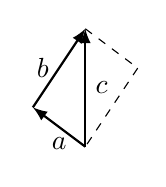
\begin{tikzpicture}
\pgfmathsetmacro{\a}{2};
\pgfmathsetmacro{\b}{1};
\pgfmathsetmacro{\c}{1.5};
\pgfmathsetmacro{\angA}{atan(\a/\c)};
\pgfmathsetmacro{\angB}{atan(\b/\c)};
\pgfmathsetmacro{\w}{0.3};
\pgfmathsetmacro{\h}{0.4};
\pgfmathsetmacro{\aa}{\c*sin(\angA)};
\pgfmathsetmacro{\bb}{\c*sin(\angB)};
%
\draw[thick,-latex](0,0)--++(90+\angA:\bb)node[pos=0.5,below]{$\bM{a}$};
\draw[thick,-latex](0,0)++(90+\angA:\bb)--++(90-\angB:\aa)node[pos=0.5,left]{$\bM{b}$}coordinate(kT);
\draw[thick,-latex] (0,0)--(kT)node[pos=0.5,right]{$\bM{c}$};
%
\draw[dashed](kT)--++(90+\angA:-\bb);
\draw[dashed](kT)++(90+\angA:-\bb)--++(90-\angB:-\aa);
\end{tikzpicture}
\caption*{(ب) سمتیوں کا مجموعہ بذریعہ متوازی الاضلاع}
\end{subfigure}%
\caption{تجربہ سے قوتوں کا مجموعہ حاصل کرتے ہوئے سمتیات کے مجموعے کا حصول حاصل ہوتا ہے۔}
\label{شکل_الجبرا_متوازی_الاضلاع_مجموعہ}
\end{figure}


\ابتدا{تعریف}\quad سمتیات کا مجموعہ\\
دو سمتیات \عددی{\bM{a}} اور \عددی{\bM{b}} کو لیتے ہوئے \عددی{\bM{a}} کے سر کے ساتھ \عددی{\bM{b}} کی دم ملائیں۔اب \عددی{\bM{a}} اور \عددی{\bM{b}} کی مجموعے کی تعریف  وہ سمتیہ \عددی{\bM{c}} ہے جو \عددی{\bM{a}} کی دم سے  \عددی{\bM{b}} کے سر تک کھینچی جائے گی (شکل \حوالہ{شکل_الجبرا_سمتیات_مجموعہ}-الف)۔اس عمل کو درج ذیل لکھا جاتا ہے۔
\begin{align}
\bM{c}=\bM{a}+\bM{b}
\end{align} 
\انتہا{تعریف}
%========================
\begin{figure}
\centering
\begin{subfigure}{0.5\textwidth}
\centering
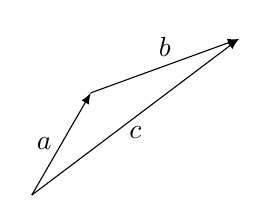
\begin{tikzpicture}
\draw[-latex](0,0)--++(60:1.5)node[pos=0.5,left]{$\bM{a}$};
\draw[-latex](0,0)++(60:1.5)--++(20:2)node[pos=0.5,above]{$\bM{b}$};
\draw[latex-](0,0)++(60:1.5)++(20:2)--(0,0)node[pos=0.5,below]{$\bM{c}$};
\end{tikzpicture}
\caption*{(الف) سر کے ساتھ دم ملا کر سمتیات کا مجموعہ حاصل کیا جاتا ہے۔}
\end{subfigure}%
\begin{subfigure}{0.5\textwidth}
\centering
\begin{tikzpicture}
\draw(0,0)--(4,0)node[below]{$x$};
\draw(0,0)--(0,2.75)node[left]{$y$};
%
\draw[-latex](0.5,0.25)coordinate(ka)--++(60:1.5)node[pos=0.5,left]{$\bM{a}$}coordinate(kb);
\draw[-latex](0.5,0.25)++(60:1.5)--++(20:2)node[pos=0.3,above]{$\bM{b}$}coordinate(kc);
\draw[latex-](0.5,0.25)++(60:1.5)++(20:2)--(0.5,0.25)node[pos=0.3,below]{$\bM{c}$};
%
\draw[dashed] (ka)--($(0,0)!(ka)!(4,0)$)coordinate(kxa)++(0,-0.6)coordinate(kkxa);
\draw[dashed] (ka)--($(0,0)!(ka)!(0,2)$)coordinate(kya)++(-0.6,0)coordinate(kkya);
\draw[dashed] (kb)--($(0,0)!(kb)!(4,0)$)coordinate(kxb);
\draw[dashed] (kb)--($(0,0)!(kb)!(0,2)$)coordinate(kyb);
\draw[dashed] (kc)--($(0,0)!(kc)!(4,0)$)coordinate(kxc)++(0,-0.6)coordinate(kkxc);
\draw[dashed] (kc)--($(0,0)!(kc)!(0,2)$)coordinate(kyc)++(-0.6,0)coordinate(kkyc);
%
\draw[thick] (kxa)--(kxb)node[pos=0.5,below]{$a_1$};
\draw[very thick] (kxb)--(kxc)node[pos=0.5,below]{$b_1$};
\draw[very thick] (kkxa)--(kkxc)node[pos=0.5,below]{$c_1$};
%
\draw[thick] (kya)--(kyb)node[pos=0.5,left]{$a_2$};
\draw[very thick] (kyb)--(kyc)node[pos=0.5,left]{$b_2$};
\draw[very thick] (kkya)--(kkyc)node[pos=0.5,left]{$c_2$};
\end{tikzpicture}
\caption*{(ب) سمتیات کے مطابقتی اجزاء کو جمع کرتے ہوئے حاصل جمع سمتیہ کے اجزاء حاصل ہوتے ہیں۔}
\end{subfigure}%
\caption{مجموعہ سمتیات۔}
\label{شکل_الجبرا_سمتیات_مجموعہ}
\end{figure}
سمتیات کی مجموعے کی تعریف سے ظاہر ہے کہ اگر کسی معین کارتیسی نظام محدد میں \عددی{\bM{a}} کے اجزاء \عددی{a_1}، \عددی{a_2} اور \عددی{a_3} جبکہ \عددی{\bM{b}} کے اجزاء \عددی{b_1}، \عددی{b_2} اور \عددی{b_3} ہوں تب حاصل جمع سمتیہ \عددی{\bM{c}} کے اجزاء \عددی{c_1}، \عددی{c_2} اور \عددی{c_3} درج ذیل ہوں گے۔
\begin{align}\label{مساوات_الجبرا_مجموعہ_سمتیات_الف}
c_1=a_1+b_1,\quad c_2=a_2+b_2,\quad c_3=a_3+b_3
\end{align}
شکل \حوالہ{شکل_الجبرا_سمتیات_مجموعہ}-ب میں اس عمل کو سطح پر دکھایا گیا ہے، اور فضا میں بھی بالکل ایسا ہی ہو گا۔

مجموعے کی تعریف یا مساوات \حوالہ{مساوات_الجبرا_مجموعہ_سمتیات_الف} سے مجموعہ سمتیات کی درج ذیل خصوصیات ملتی ہیں جہاں \عددی{-\bM{a}} سے مراد ایسا سمتیہ ہے جس کی لمبائی \عددی{\abs{\bM{a}}} اور سمت \عددی{\bM{a}} کے الٹ ہو۔
\begin{gather}
\begin{aligned}\label{مساوات_الجبرا_سمتیات_مجموعہ_قواعد_الف}
\text{(الف)}\quad \quad \bM{a}+\bM{b}&=\bM{b}+\bM{a}\quad \text{\RL{قانون تبادل}}\\
\text{(ب)}\quad (\bM{u}+\bM{v})+\bM{w}&=\bM{u}+(\bM{v}+\bM{w})\quad \text{\RL{قانون تلازم}}\\
\text{(پ)}\quad \quad \bM{a}+\bM{0}&=\bM{0}+\bM{a}\\
\text{(ت)}\quad \quad \bM{a}+(-\bM{a})&=\bM{0}
\end{aligned}
\end{gather}
مساوات \حوالہ{مساوات_الجبرا_سمتیات_مجموعہ_قواعد_الف}-ب میں ہم \عددی{\bM{u}+\bM{v}+\bM{w}} لکھ سکتے ہیں اور یہی طریقہ زیادہ اعداد کے سمتیات کا مجموعہ لکھنے  کے لئے بھی استعمال کیا جاتا ہے۔مجموعہ \عددی{\bM{a}+\bM{a}} کی جگہ \عددی{2\bM{a}} لکھا جاتا ہے، وغیرہ، وغیرہ۔ ان سے (اور \عددی{-\bM{a}} کے استعمال سے) ہم سمتیات کا دوسرا الجبرائی عمل بیان کرتے ہیں۔

\جزوحصہء{سمتیات کا غیر سمتیات (اعداد) کے ساتھ ضرب}
اگر \عددی{\bM{a}} ایک سمتیہ اور \عددی{q} کوئی حقیقی عدد ہو تب سمتیہ \عددی{q\bM{a}} کی تعریف درج ذیل ہے۔

\begin{itemize}
\item[]
\عددی{q\bM{a}} کی لمبائی \عددی{\abs{q}\abs{\bM{a}}} ہے۔
\item[]
اگر \عددی{\bM{a} \ne \bM{0}} ہو اور \عددی{q>0} ہو تب \عددی{q\bM{a}} کی سمت وہی ہو گی جو \عددی{\bM{a}} کی تھی۔
\item[]
اگر \عددی{\bM{a} \ne \bM{0}} ہو اور \عددی{q<0} ہو تب \عددی{q\bM{a}} کی سمت \عددی{\bM{a}} کی سمت کے الٹ ہو گی۔
\item[]
اگر \عددی{\bM{a}=\bM{0}} یا \عددی{q=0} ہو (اور یا دونوں صفر ہوں) تب \عددی{q\bM{a}=\bM{0}} ہو گا۔
\end{itemize}
%========================================

ان قواعد کی سادہ مثالیں شکل \حوالہ{شکل_الجبرا_سمتیات_اور_غیر_سمتیات_کا_ضرب}-الف میں دکھائی گئی ہے۔
\begin{figure}
\centering
\begin{subfigure}{0.5\textwidth}
\centering
\begin{tikzpicture}
\draw[-latex](0,0)node[below]{$\bM{a}$}--++(30:1);
\draw[-latex](1,0)node[below]{$\tfrac{1}{2}\bM{a}$}--++(30:0.5);
\draw[latex-](2,0)node[below]{$-\bM{a}$}--++(30:1);
\draw[-latex](3,0)node[below]{$2\bM{a}$}--++(30:2);
\draw[latex-](4,0)node[below]{$-\tfrac{1}{2}\bM{a}$}--++(30:0.5);
\end{tikzpicture}
\caption*{(الف) سمتیات کا غیر سمتیات کے ساتھ ضرب۔}
\end{subfigure}%
\begin{subfigure}{0.5\textwidth}
\centering
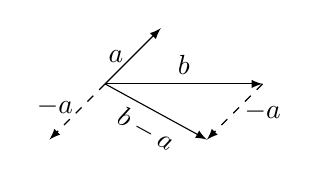
\begin{tikzpicture}
\draw[-latex](0,0)--++(2,0)node[above,pos=0.5]{$\bM{b}$};
\draw[-latex](0,0)--++(45:1)node[left,pos=0.5]{$\bM{a}$};
\draw[-latex,dashed](0,0)--++(45:-1)node[left,pos=0.4]{$-\bM{a}$};
\draw[-latex,dashed](0,0)++(2,0)--++(45:-1)node[pos=0.5,right]{$-\bM{a}$}coordinate(kT);
\draw[-latex](0,0)--(kT)node[midway, below, sloped]{$\bM{b}-\bM{a}$};
\end{tikzpicture}
\caption*{(ب) سمتیات کا فرق}
\end{subfigure}%
\caption{سمتیات کا غیر سمتیہ کے ساتھ ضرب اور سمتیات کا فرق۔}
\label{شکل_الجبرا_سمتیات_اور_غیر_سمتیات_کا_ضرب}
\end{figure}

ظاہر ہے کہ اگر \عددی{\bM{a}} کے اجزاء \عددی{a_1}، \عددی{a_2} اور \عددی{a_3} ہوں تب اسی نظام محدد میں  \عددی{q\bM{a}} کے اجزاء \عددی{qa_1}، \عددی{qa_2} اور \عددی{qa_3} ہوں گے۔اسی طرح سمتیہ کی تعریف سے  درج ذیل ہو گا۔
\begin{gather}
\begin{aligned}\label{مساوات_الجبرا_سمتیات_مجموعہ_قواعد_ب}
q(\bM{a}+\bM{b})&=q\bM{a}+q\bM{b}\\
(c+k)\bM{a}&=c\bM{a}+k\bM{a}\\
c(k\bM{a})&=(ck)\bM{a}\quad \quad \text{\RL{جس کو \عددی{ck\bM{a}} لکھا جاتا ہے}}\\
1\bM{a}&=\bM{a}
\end{aligned}
\end{gather} 
مساوات \حوالہ{مساوات_الجبرا_سمتیات_مجموعہ_قواعد_الف} اور مساوات \حوالہ{مساوات_الجبرا_سمتیات_مجموعہ_قواعد_ب} سے درج ذیل اخذ کیا جا سکتا ہے۔
\begin{gather}
\begin{aligned}
0\bM{a}&=\bM{0}\\
(-1)\bM{a}&=-\bM{a}
\end{aligned}
\end{gather}
ہم \عددی{ \bM{b}-(\bM{a})} کی جگہ \عددی{\bM{b}-\bM{a}} لکھ سکتے ہیں (شکل \حوالہ{شکل_الجبرا_سمتیات_اور_غیر_سمتیات_کا_ضرب}-ب)۔

کسی بھی ایک کارتیسی نظام محدد کو استعمال کرتے ہوئے، ہم سمتیہ \عددی{\bM{a}} جس کے اجزاء \عددی{a_1}، \عددی{a_2} اور \عددی{a_3}  ہوں کو تین ایسی سمتیات کا مجموعہ لکھ سکتے ہیں جو اس کارتیسی نظام کے تین محور کے متوازی ہوں۔ہم اس کارتیسی نظام کے ساتھ تین ایسے اکائی سمتیات، جنہیں ہم \عددی{\bM{i}}، \عددی{\bM{j}} اور \عددی{\bM{k}} کہیں گے، وابستہ کرتے ہیں جن کی مثبت سمت اس کارتیسی نظام کے محور کی مثبت سمت ہو۔ یوں   \عددی{\bM{a}} کو درج ذیل لکھا جا سکتا ہے (شکل \حوالہ{شکل_الجبرا_اکائی_سمتیات})۔
\begin{align}
\bM{a}=a_1\bM{i}+a_2\bM{j}+a_3\bM{k}
\end{align}
\begin{figure}
\centering
\begin{subfigure}{0.5\textwidth}
\centering
\begin{tikzpicture}[x={(-0.5cm,-0.5cm)},y={(1cm,0)},z={(0,1cm)}]
\draw(0,0,0)--++(2,0,0)node[left]{$x$};
\draw(0,0,0)--++(0,2,0)node[below]{$y$};
\draw(0,0,0)--++(0,0,1.5)node[left]{$z$};
%
\draw[-latex,thick](0,0,0)--++(0.75,0,0)node[above left]{$\bM{i}$};
\draw[-latex,thick](0,0,0)--++(0,0.75,0)node[below,pos=0.8]{$\bM{j}$};
\draw[-latex,thick](0,0,0)--++(0,0,0.75)node[left,pos=0.8]{$\bM{k}$};
\end{tikzpicture}
\caption*{(الف) اکائی سمتیات \عددی{\bM{i}}، \عددی{\bM{j}} اور \عددی{\bM{k}}}
\end{subfigure}%
\begin{subfigure}{0.5\textwidth}
\centering
\begin{tikzpicture}[x={(-0.5cm,-0.5cm)},y={(1cm,0)},z={(0,1cm)}]
\draw(0,0,0)--++(2.25,0,0)node[left]{$x$};
\draw(0,0,0)--++(0,2.5,0)node[below]{$y$};
\draw(0,0,0)--++(0,0,2.25)node[left]{$z$};
%
\draw[dashed,gray] (1.25,2,1.75)--++(-1.25,0,0)--++(0,0,-1.75)--++(1.25,0,0);
\draw[dashed,gray](1.25,2,1.75)--++(0,-2,0)--++(-1.25,0,0)--++(0,2,0)--++(1.25,0,0);
\draw[dashed,gray](1.25,0,0)--++(0,0,1.75);
%
\draw[-latex,thick](0,0,0)--(1.25,0,0)node[above left,pos=0.7]{$a_1\bM{i}$};
\draw[-latex,thick](1.25,0,0)--(1.25,2,0)node[below,pos=0.5]{$a_2\bM{j}$};
\draw[-latex,thick](1.25,2,0)--(1.25,2,1.75)node[right,pos=0.6]{$a_3\bM{k}$};
\draw[-latex,thick](0,0,0)node[ocirc]{}--(1.25,2,1.75)node[pos=0.6,left]{$\bM{a}$};
\end{tikzpicture}
\caption*{(ب) سمتیہ کا تین اکائی سمتیات کی مدد سے اظہار}
\end{subfigure}%
\caption{اکائی سمتیات اور ان کا استعمال۔}
\label{شکل_الجبرا_اکائی_سمتیات}
\end{figure}
شکل \حوالہ{شکل_الجبرا_اکائی_سمتیات}-الف میں اکائی سمتیات \عددی{\bM{i}}، \عددی{\bM{j}} اور \عددی{\bM{k}} کو دکھایا گیا ہے جہاں ان   کی دم کو کارتیسی نظام کے مرکز پر رکھا گیا ہے۔یہ اکائی سمتیات آپس میں \ترچھا{عمودی} یا \اصطلاح{قائمہ}\فرہنگ{قائمہ}\حاشیہب{orthogonal}\فرہنگ{orthogonal} ہیں۔ہم کہتے ہیں کہ \عددی{\bM{i}}، \عددی{\bM{j}} اور \عددی{\bM{k}} اس نظام محدد کی \ترچھا{ثلاثہ اکائی قائمہ سمتیات}\فرہنگ{ثلاثہ قائمہ سمتیات}  ہیں۔

کسی بھی سمتیہ کو اس کی لمبائی سے تقسیم کرتے ہوئے اسی سمت میں اکائی سمتیہ حاصل ہو گا۔یوں \عددی{\bM{a}} کی سمت میں اکائی سمتیہ درج ذیل ہو گا۔
\begin{align}\label{مساوات_الجبرا_اکائی_سمتیہ_حصول}
\text{\RL{اکائی سمتیہ}}=\frac{\bM{a}}{\abs{\bM{a}}}
\end{align}
%================
\ابتدا{مثال}
کسی کارتیسی نظام میں اگر \عددی{\bM{a}=3\bM{i}-2\bM{k}} اور \عددی{\bM{b}=-5\bM{i}+4\bM{j}+2\bM{k}} ہوں، تب درج ذیل ہوں گے۔
\begin{align*}
3\bM{a}=9\bM{i}-6\bM{k},\quad -\bM{b}=5\bM{i}-4\bM{j}-2\bM{k},\quad 1.2\bM{a}-0.5\bM{b}=6.1\bM{i}-2\bM{j}-3.4\bM{k}
\end{align*}
\انتہا{مثال}
%============================
\ابتدا{مثال}
کسی سمتیہ{\bM{a}} کی دم \عددی{A} پر ہے جبکہ اس کا سر \عددی{B} پر ہے۔اسی سمت میں کسی بھی  سمتیہ  کو \عددی{l\bM{a}} لکھا جا سکتا ہے جہاں \عددی{l} غیر سمتی مستقل ہے۔اب اگر \عددی{l\bM{a}} سمتیہ کی دم  \عددی{A} پر ہو تب  \عددی{l=0} کی صورت میں اس سمتیہ کا سر نقطہ \عددی{A} پر ہو گا جبکہ \عددی{l=1} کی صورت میں اس کا سر نقطہ \عددی{B} پر ہو گا۔اسی طرح \عددی{l=\tfrac{1}{2}} کی صورت میں اس سمتیہ کا سر \عددی{\bM{a}} کے عین وسط پر ہو گا۔

\انتہا{مثال}
%==============================
\ابتدا{مثال}\quad اکائی سمتیہ\\
سمتیہ \عددی{\bM{a}=2\bM{i}-5\bM{j}+3\bM{k}} کی سمت میں اکائی سمتیہ دریافت کریں۔اسی سمت میں ایسا سمتیہ حاصل کریں جس کی لمبائی \عددی{7} ہو۔

حل:\عددی{\bM{a}} کی لمبائی \عددی{\abs{\bM{a}}=\sqrt{4+25+9}=\sqrt{38}} ہے۔یوں مساوات \حوالہ{مساوات_الجبرا_اکائی_سمتیہ_حصول} کے تحت \عددی{\bM{a}} کی سمت میں اکائی سمتیہ
\begin{align*}
\frac{\bM{a}}{\abs{\bM{a}}}=\frac{2\bM{i}-5\bM{j}+3\bM{k}}{\sqrt{38}}
\end{align*}
ہو گا۔کسی بھی اکائی سمتیہ کو غیر سمتی \عددی{l} سے ضرب دینے سے اس اکائی سمتیہ کی سمت میں \عددی{l} لمبائی کا سمتیہ حاصل ہوتا ہے لہٰذا درکار سمتیہ درج ذیل ہو گا۔
\begin{align*}
7\frac{\bM{a}}{\abs{\bM{a}}}=\frac{14\bM{i}-35\bM{j}+21\bM{k}}{\sqrt{38}}=2.27\bM{i}-6.68\bM{j}+3.41\bM{k}
\end{align*}
\انتہا{مثال}
%=======================
\ابتدا{مثال}\شناخت{مثال_الجبرا_سمتیات_کا_استعمال}
\عددی{\bM{a}}، \عددی{\bM{b}} اور \عددی{\bM{c}} شکل \حوالہ{شکل_مثال_الجبرا_سمتیات_کا_استعمال} -الف میں دکھائے گئے چپٹا  ڈبے کے تین قریبی کنارے ہیں۔ڈبے کی سامنے سطح \عددی{mnqp} کا وتر \عددی{\bM{v}_{mq}} اور \عددی{\bM{v}_{np}} دریافت کریں جہاں وتر \عددی{\bM{v}_{mq}} کی دم \عددی{q}  اور سر \عددی{m} ہیں۔جیسا شکل \حوالہ{شکل_مثال_الجبرا_سمتیات_کا_استعمال} -ب میں دکھایا گیا ہے، وتری سمتیات \عددی{\bM{v}_{mq}} اور \عددی{\bM{v}_{np}} ایک دونوں کو نقطہ \عددی{t} پر قطع کرتے ہیں۔نقطہ \عددی{t} دریافت کرتے ہوئے ثابت کریں کہ دونوں وتر ایک دونوں کو برابر حصوں میں قطع کرتے ہیں۔
\begin{figure}
\centering
\begin{subfigure}{0.5\textwidth}
\centering
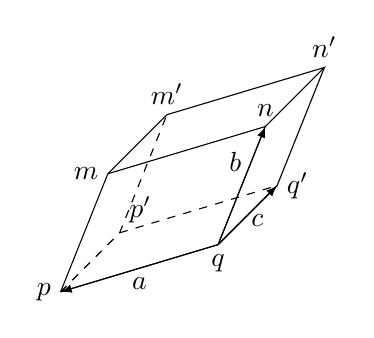
\begin{tikzpicture}[x={(-0.5cm,-0.5cm)},y={(1cm,0.3cm)},z={(0.4cm,1cm)}]
\pgfmathsetmacro{\a}{1.5}
\pgfmathsetmacro{\b}{2}
\pgfmathsetmacro{\c}{1.5}
%box
\draw(\a,0,0)node[left]{$p$}--++(0,\b,0)node[below]{$q$}--++(0,0,\c)node[above]{$n$}--++(0,-\b,0)node[left]{$m$}--++(0,0,-\c);
\draw(\a,0,\c)--++(-\a,0,0)node[above]{$m'$}--++(0,\b,0)node[above]{$n'$}--++(\a,0,0);
\draw(\a,\b,0)--++(-\a,0,0)--++(0,0,\c);
\draw[dashed] (\a,0,0)--++(-\a,0,0)--++(0,0,\c);
\draw[dashed](0,0,0)node[above right]{$p'$}--++(0,\b,0)node[right]{$q'$};
%edge vectors
\draw[-latex] (\a,\b,0)--++(0,-\b,0)node[pos=0.5,below]{$\bM{a}$};
\draw[-latex] (\a,\b,0)--++(0,0,\c)node[pos=0.7,left]{$\bM{b}$};
\draw[-latex] (\a,\b,0)--++(-\a,0,0)node[pos=0.4,right]{$\bM{c}$};
\end{tikzpicture}
\caption*{(الف) چپٹا ڈبا۔}
\end{subfigure}%
\begin{subfigure}{0.5\textwidth}
\centering
\begin{tikzpicture}[x={(-0.5cm,-0.5cm)},y={(1cm,0.3cm)},z={(0.4cm,1cm)}]
\pgfmathsetmacro{\a}{1.5}
\pgfmathsetmacro{\b}{2}
\pgfmathsetmacro{\c}{1.5}
%box
\draw(\a,0,0)--++(0,0,\c)node[left]{$m$}--++(0,\b,0)node[right]{$n$}--++(0,0,-\c);
%edge vectors
\draw[-latex] (\a,\b,0)node[below]{$q$}--++(0,-\b,0)node[below]{$p$}node[pos=0.5,below]{$\bM{a}$};
\draw[-latex] (\a,\b,0)--++(0,0,\c)node[pos=0.5,right]{$\bM{b}$};
\draw[] (\a,\b/2,\c/2) node[circ]{}node[above]{$t$};
%diagonals
\draw[-latex](\a,\b,0)--++(0,-\b,\c);
\draw[-latex](\a,0,0)--++(0,\b,\c);
\draw[-latex,thick](\a,\b,0)--++(0,-\b/2,\c/2);
\end{tikzpicture}
\caption*{(ب) وتر نقطہ \عددی{t} پر ایک دونوں کو  برابر حصوں میں قطع کرتے ہیں۔}
\end{subfigure}%
\caption{سمتیات کا استعمال۔ مثال \حوالہ{مثال_الجبرا_سمتیات_کا_استعمال}}
\label{شکل_مثال_الجبرا_سمتیات_کا_استعمال}
\end{figure}

حل:شکل کو دیکھ کر درج ذیل لکھا جا سکتا ہے۔
\begin{align*}
\bM{r}_{mq}=\bM{a}+\bM{c},\quad \bM{r}_{np}=-\bM{a}+\bM{c}
\end{align*}
شکل \حوالہ{شکل_مثال_الجبرا_سمتیات_کا_استعمال}-ب سے ظاہر ہے کہ \عددی{q} کو ابتدائی نقطہ تصور کرتے ہوئے \عددی{t} تک کئی راستوں سے پہنچا جا سکتا ہے۔ چونکہ  \عددی{t} وتر \عددی{\bM{v}_{mq}} پر پایا جاتا ہے لہٰذا \عددی{q} سے \عددی{t} تک سمتیہ  کو \عددی{\bM{v}_{tq}=l_1\bM{v}_{mq}} لکھا جا سکتا ہے جہاں \عددی{0<l_1<1} ممکن ہے۔اسی طرح  \عددی{q} سے پہلے \عددی{p} اور یہاں سے \عددی{\bM{v}_{np}} می سمت میں چلتے ہوئے بھی نقطہ \عددی{t} تک پہنچنا ممکن ہے۔ایسا کرتے ہوئے 
\عددی{\bM{v}_{tq}=\bM{a}+l_2\bM{v}_{np}} لکھا جا سکتا ہے جہاں \عددی{0<l_2<1} ممکن ہے۔یوں درج ذیل ہو گا
\begin{align}\label{مساوات_الجبرا_مثال_وتری_قطع}
\bM{v}_{tq}=l_1\bM{v}_{mq}=\bM{a}+l_2\bM{v}_{np}\quad \implies l_1(\bM{a}+\bM{c})=\bM{a}+l_2(-\bM{a}+\bM{c})
\end{align}
جس کو ترتیب دیتے ہوئے
\begin{align*}
\bM{a}(l_1-1+l_2)+\bM{c}(l_1-l_2)=0
\end{align*}
ملتا ہے۔اب چونکہ \عددی{\bM{a}} اور \عددی{\bM{b}} غیر صفر ہیں اور ان کی سمتیں بھی مختلف ہیں لہٰذا درج بالا مساوات صرف اور صرف اس صورت ممکن ہو گا جب دونوں قوسین صفر ہوں یعنی:
\begin{align*}
l_1-1+l_2&=0\\
l_1-l_2&=0
\end{align*}
ان ہمزاد مساوات کو حل کرتے ہوئے \عددی{l_1=l_2=\tfrac{1}{2}} ملتا ہے۔اب \عددی{l_1=\tfrac{1}{2}} کی صورت میں مساوات \حوالہ{مساوات_الجبرا_مثال_وتری_قطع} سے  
\عددی{\bM{v}_{tq}=\tfrac{1}{2}\bM{v}_{mq}}ملتا  ہے جس کا مطلب ہے کہ نقطہ \عددی{t} عین \عددی{mq} کے وسط میں پایا جاتا ہے۔ مساوات \حوالہ{مساوات_الجبرا_مثال_وتری_قطع} کے اگلے حصے سے اسی طرح ثابت ہوتا ہے کہ نقطہ \عددی{t} عین \عددی{np} کے وسط میں پایا جاتا ہے۔

\انتہا{مثال}
%========================
\حصہء{سوالات}
سوال \حوالہ{سوال_الجبرا_سمتیات_اعمال_جمع_الف} تا سوال \حوالہ{سوال_الجبرا_سمتیات_اعمال_جمع_ب} میں \عددی{\bM{a}=2\bM{i}-\bM{j}+\bM{k}}، \عددی{\bM{b}=-3\bM{i}-2\bM{j}+4\bM{k}} اور \عددی{\bM{c}=-2\bM{k}} لیں۔

%===========
\ابتدا{سوال}\شناخت{سوال_الجبرا_سمتیات_اعمال_جمع_الف}\quad
$-4\bM{a},\tfrac{1}{4}\bM{a},4\bM{a}$\\
جوابات:
$-4\bM{a}=-8\bM{i}+4\bM{j}-4\bM{k},\, \tfrac{1}{4}\bM{a}=\tfrac{1}{2}\bM{i}-\tfrac{1}{4}\bM{j}+\tfrac{1}{4}\bM{k},4\bM{a}=8\bM{i}-4\bM{j}+4\bM{k}$
\انتہا{سوال}
%===================
\ابتدا{سوال}\quad
$\bM{a}+\bM{b},\bM{b}+\bM{a}$\\
جوابات:
$-\bM{i}-3\bM{j}+5\bM{k}$
\انتہا{سوال}
%===================
\ابتدا{سوال}\quad
$\bM{a}-\bM{b},\bM{b}-\bM{a}, \bM{a}-\bM{b}-\bM{c}$\\
جوابات:
$\bM{a}-\bM{b}=5\bM{i}+\bM{j}-3\bM{k}, \,\bM{b}-\bM{a}=-5\bM{i}-\bM{j}+3\bM{k},\, \bM{a}-\bM{b}-\bM{c}=5\bM{i}+\bM{j}-\bM{k}$
\انتہا{سوال}
%===================
\ابتدا{سوال}\quad
$\abs{\bM{a}-\bM{b}},\abs{\bM{b}-\bM{a}}, \abs{\bM{a}-\bM{b}-\bM{c}}$\\
جوابات:
$\sqrt{35}, \sqrt{35}, 3^{\tfrac{3}{2}}$
\انتہا{سوال}
%===================
\ابتدا{سوال}\quad
$\abs{\bM{a}+\bM{b}},\abs{\bM{a}}+\abs{\bM{b}}$\\
جوابات:
$5.916, 7.835$
\انتہا{سوال}
%===================
\ابتدا{سوال}\quad
$\abs{\bM{a}-\bM{b}},\abs{\bM{a}}-\abs{\bM{b}}$\\
جوابات:
$5.916, -2.936$
\انتہا{سوال}
%===================
\ابتدا{سوال}\quad
$\frac{\bM{a}}{\abs{\bM{a}}},\frac{\bM{b}}{\abs{\bM{b}}},\frac{\bM{c}}{\abs{\bM{c}}}$\\
جوابات:
$0.82\bM{i}-0.41\bM{j}+0.41\bM{k},\, -0.56\bM{i}-0.31\bM{j}+0.74\bM{k},\, -\bM{k}$
\انتہا{سوال}
%===================
\ابتدا{سوال}\quad
$\frac{\bM{a}+\bM{c}}{\abs{\bM{a}+\bM{c}}},\frac{\bM{b}-\bM{c}}{\abs{\bM{b}-\bM{c}}},\frac{\bM{a}+\bM{b}+\bM{c}}{\abs{\bM{a}+\bM{b}+\bM{c}}}$\\
جوابات:
$-0.17\bM{i}-0.51\bM{j}+0.85\bM{k},\, -0.43\bM{i}-0.29\bM{j}+0.86\bM{k},\, -0.23\bM{i}-0.69\bM{j}+0.69\bM{k}$
\انتہا{سوال}
%===================
\ابتدا{سوال}\quad
$(\bM{a}+\bM{b})+\bM{c}, \bM{a}+(\bM{b}+\bM{c})$\\
جوابات:
$-\bM{i}-3\bM{j}+3\bM{k}$
\انتہا{سوال}
%===================
\ابتدا{سوال}\شناخت{سوال_الجبرا_سمتیات_اعمال_جمع_ب}\quad
$4(\bM{a}-\bM{b}), 4\bM{a}-4\bM{b}$\\
جوابات:
$20\bM{i}+4\bM{j}-12\bM{k}$
\انتہا{سوال}
%===================
\ابتدا{سوال}
قوت \عددی{\bM{n}=2\bM{i}-\bM{j}-3\bM{k}}  اور \عددی{\bM{p}=-3\bM{i}-2\bM{j}+7\bM{k}} ہیں۔ایسی قوت \عددی{\bM{m}} دریافت کریں کہ \عددی{\bM{m}}، \عددی{\bM{n}} اور \عددی{\bM{p}}  توازن میں ہوں۔ 

جواب:\عددی{\bM{m}=\bM{i}+3\bM{j}-4\bM{k}}
\انتہا{سوال}
%=========================
\ابتدا{سوال}
ثابت کریں کہ شکل \حوالہ{شکل_مثال_الجبرا_سمتیات_کا_استعمال} میں وتر \عددی{m'q} اور \عددی{n'p} ایک دونوں کو برابر حصوں میں تقسیم کرتے ہیں۔

جواب:\عددی{\bM{v}_{m'q}=\bM{a}+\bM{b}+\bM{c}} اور \عددی{\bM{v}_{n'p}=-\bM{a}+\bM{b}+\bM{c}} ہیں۔اب
 \عددی{\bM{v}_{tq}=l_1\bM{v}_{m'q}} اور اسی طرح \عددی{\bM{v}_{tq}=\bM{a}+l_2\bM{v}_{n'p}} لکھا جا سکتا ہے۔انہیں برابر پر کرتے ہوئے
\begin{align*}
l_1(\bM{a}+\bM{b}+\bM{c})=\bM{a}+l_2(-\bM{a}+\bM{b}+\bM{c})
\end{align*}
 یعنی \عددی{\bM{a}(l_1-1+l_2)+\bM{b}(l_1-l_2)+\bM{c}(l_1-l_2)=0} ملتا ہے۔چونکہ سمتیات صفر نہیں ہیں لہٰذا قوسین صفر ہوں گے۔یوں حاصل ہمزاد مساوات \عددی{l_1-1+l_2=0} اور \عددی{l_1-l_2=0} حل کرتے ہوئے \عددی{l_1=l_2=\tfrac{1}{2}} ملتا ہے۔
\انتہا{سوال}
%=========================
\ابتدا{سوال}\شناخت{سوال_الجبرا_تکون_قطع}
تکون کی تین کونوں سے سامنے اطراف کی وسط کو ملانے والے خط ایک دونوں کو نقطہ \عددی{t} پر قطع کرتے ہیں۔ \عددی{t} کے دونوں اطراف، خط کی لمبائی کا نسبت دریافت کریں۔ 

جواب:تکون کو شکل \حوالہ{شکل_سوال_الجبرا_تکون_قطع}-الف میں دکھایا گیا ہے جہاں \عددی{mn} کی وسط پر نقطہ \عددی{p'} اور \عددی{pn} کی وسط پر نقطہ \عددی{m'} دکھائے گئے ہیں۔یوں سمتیہ \عددی{\bM{v}_{m'n}} جس کی دم نقطہ \عددی{n} پر ہے کو \عددی{\bM{v}_{m'n}=\tfrac{1}{2}(\bM{b}-\bM{a})} لکھا جا سکتا ہے جس کو استعمال کرتے ہوئے \عددی{\bM{v}_{m'm}=\bM{a}+\bM{v}_{m'n}} لکھا جا سکتا ہے۔اسی طرح \عددی{\bM{v}_{p'p}=\tfrac{1}{2}\bM{a}-\bM{b}} لکھا جا سکتا ہے۔انہیں استعمال کرتے ہوئے \عددی{\bM{v}_{tm}=\bM{b}+l_1\bM{v}_{p'p}} اور \عددی{\bM{v}_{tm}=l_2\bM{v}_{m'm}} لکھے جا سکتے ہیں۔انہیں حل کرتے ہوئے \عددی{l_1=l_2=\tfrac{2}{3}} ملتا ہے۔یوں \عددی{m'm} خط کے دو حصوں کا تناسب \عددی{\tfrac{2}{3}} اور \عددی{\tfrac{1}{3}}  یعنی \عددی{2:1} ہو گا۔
\begin{figure}
\centering
\begin{subfigure}{0.5\textwidth}
\centering
\begin{tikzpicture}
\draw[-latex](0,0)coordinate(m)node[left]{$m$}--++(10:2)node[right]{$n$}node[pos=0.75,below]{$\bM{a}$}coordinate(n);
\draw[-latex](0,0)--++(60:1.5)node[above]{$p$}node[pos=0.5,above left]{$\bM{b}$}coordinate(p);
\draw[](n)--(p);
\draw[name path=aa](m)--($(n)!0.5!(p)$)node[above right]{$m'$}coordinate(mA);
\draw[name path=bb](p)--($(n)!0.5!(m)$)node[below]{$p'$};
\draw[name intersections={of={aa and bb}}] (intersection-1)node[ocirc]{}node[shift={(-30:0.2)}]{$t$};
\end{tikzpicture}
\caption*{(الف) سوال \حوالہ{سوال_الجبرا_تکون_قطع} کی شکل۔}
\end{subfigure}%
\begin{subfigure}{0.5\textwidth}
\centering
\begin{tikzpicture}
\draw(0,0)node[below]{$A(1,-2,4)$}--(2,0.5)node[ocirc]{}node[below]{$B(5,1,3)$}--(1,2)node[ocirc]{}node[above]{$C(2,3,1)$}--(0,0)node[ocirc]{};
\draw(0,0)--($(2,0.5)!0.7!(1,2)$)node[ocirc]{}node[right]{$D$};
\end{tikzpicture}
\caption*{(ب) سوال \حوالہ{سوال_الجبرا_تکون_سمتیہ} کی شکل۔}
\end{subfigure}%
\caption{سمتیات کا استعمال۔}
\label{شکل_سوال_الجبرا_تکون_قطع}
\end{figure}

\انتہا{سوال}
%===========================
\ابتدا{سوال}\شناخت{سوال_الجبرا_تکون_سمتیہ}
تکون کے کونے \عددی{A(1,-2,4)}، \عددی{B(5,1,3)} اور \عددی{C(2,3,1)} ہیں۔\عددی{BC} پر \عددی{D} پایا جاتا ہے جہاں
 \عددی{\overline{BD}=2\overline{CD}} ہے۔اس کو شکل \حوالہ{سوال_الجبرا_تکون_سمتیہ}-ب میں دکھایا گیا ہے۔خط \عددی{AD} کی لمبائی دریافت کریں۔

جواب:\عددی{\bM{v}_{BA}=4\bM{i}+3\bM{j}-\bM{k}} اور \عددی{\bM{v}_{CB}=-3\bM{i}+2\bM{j}-2\bM{k}} ہیں۔اب دی گئی معلومات کے تحت \عددی{\bM{v}_{DB}=\tfrac{2}{3}\bM{v}_{CB}} ہے۔یوں \عددی{\bM{v}_{DA}=\bM{v}_{BA}+\bM{v}_{DB}} یعنی \عددی{\bM{v}_{AD}=2\bM{i}+\tfrac{13}{3}\bM{j}-\tfrac{7}{3}\bM{k}} ہو گا جس کی لمبائی \عددی{\tfrac{\sqrt{254}}{3}} ہے۔
\انتہا{سوال}
%============================
\ابتدا{سوال}
ثابت کریں کہ متوازی الاضلاع کے ایک کونے سے سامنے والی طرف کی وسط تک لکیر، وتر کو \عددی{1:2} تناسب میں تقسیم کرتی ہے۔
\انتہا{سوال}
%=============================
سوال \حوالہ{سوال_الجبرا_اکائی_سمتیہ_حصول_الف} تا سوال \حوالہ{سوال_الجبرا_اکائی_سمتیہ_حصول_ب} میں \عددی{\bM{a}} کی سمت میں اکائی سمتیہ حاصل کریں۔اس اکائی سمتیہ کی سمت میں \عددی{l} لمبائی کا سمتیہ حاصل کریں۔ظاہر ہے کہ اکائی سمتیہ کو \عددی{-1} سے ضرب دے کر الٹ سمت میں اکائی سمتیہ حاصل ہو گا۔ 

%================
\ابتدا{سوال}\شناخت{سوال_الجبرا_اکائی_سمتیہ_حصول_الف}\quad  
$\bM{a}=4\bM{j},\,\,  l=5$\\
جوابات:\عددی{\bM{j}}، \عددی{5\bM{j}}
\انتہا{سوال}
%==============================
\ابتدا{سوال}\quad  
$\bM{a}=-2\bM{i}+\bM{j}+3\bM{k},\,\, l=2$\\
جوابات:
$-3.74\bM{i}+1.87\bM{j}+5.61\bM{k},\,\,-0.535\bM{i}+0.267\bM{j}+0.802\bM{k}$
\انتہا{سوال}
%==============================
\ابتدا{سوال}\شناخت{سوال_الجبرا_اکائی_سمتیہ_حصول_ب}\quad  
$\bM{a}=\bM{b}+2\bM{c},\,\,\bM{b}=3\bM{i}+2\bM{k},\, \bM{c}=2\bM{i}-\bM{j}-\bM{k},\,\,  l=10$\\
جوابات:
$9.61\bM{i}-2.74\bM{j},\,\,0.96\bM{i}-0.27\bM{j}$
\انتہا{سوال}
%==============================

\حصہ{سمتی فضا۔خطی تابعیت اور غیر تابعیت}\شناخت{حصہ_الجبرا_سمتیات_فضا_تابعیت}
ایسے تمام سمتیات کا سلسلہ \عددی{V} جو سمتی مجموعہ (مساوات \حوالہ{مساوات_الجبرا_سمتیات_مجموعہ_قواعد_الف}) اور سمتی ضرب (مساوات \حوالہ{مساوات_الجبرا_سمتیات_مجموعہ_قواعد_ب}) کے الجبرائی قواعد پر پورا اترتا ہو کو \اصطلاح{سمتی فضا}\فرہنگ{سمتی!فضا}\فرہنگ{فضا!سمتی}\حاشیہب{vector space}\فرہنگ{vector space}\فرہنگ{space!vector} یا \اصطلاح{خطی فضا}\فرہنگ{خطی !فضا}\فرہنگ{فضا!خطی}\حاشیہب{linear space}\فرہنگ{linear!space}\فرہنگ{space!linear}  کہتے ہیں۔سمتی فضا کا تصور اس لئے اہم ہے کہ عملی دلچسپی کے دیگر \اصطلاح{سلسلے}  جو قالب، تفاعل، تبادل وغیرہ پر مبنی ہوں پائے جاتے ہیں جن کے مجموعے اور غیر سمتی ضرب کی بالکل ایسی ہی فطری  تعریف کی جا سکتی ہے۔      

%=================
\ابتدا{مسئلہ}\quad حقیقی سمتی فضا\\
اگر سلسلہ \عددی{V} کے ارکان \عددی{\bM{a}}، \عددی{\bM{b}}، \نقطے درج ذیل دو الجبرائی اعمال (جنہیں سمتی جمع اور غیر سمتی ضرب کہتے ہیں) پر پورا اترتے ہوں 
  تب \عددی{V} \اصطلاح{حقیقی سمتی فضا}\فرہنگ{حقیقی سمتی فضا}\فرہنگ{سمتی فضا!حقیقی}\حاشیہب{real vector space}\فرہنگ{vector space!real} یا \ترچھا{حقیقی خطی فضا} کہلاتا ہے  اور  یہ ارکان (جن کے خصوصیات کچھ بھی ہو سکتے ہیں)  \اصطلاح{سمتیات} کہلاتے ہیں۔

(الف)\quad \اصطلاح{سمتی جمع}\فرہنگ{سمتی!جمع}\فرہنگ{جمع!سمتی} \عددی{V} کے ہر دو سمتیات \عددی{\bM{a}} اور \عددی{\bM{b}} کے ساتھ \عددی{V} کا ایسا منفرد رکن، جو \عددی{\bM{a}} اور \عددی{\bM{b}} کا مجموعہ کہلاتا  اور \عددی{\bM{a}+\bM{b}} سے ظاہر کیا جاتا ہے،  وابستہ  کرتا ہے کہ جو درج ذیل مسلمات پر پورا اترتا ہو۔

(الف-1) \quad \اصطلاح{قانون تبادل}\فرہنگ{قانون!تبادل}۔  \عددی{V} کے ہر دو ارکان \عددی{\bM{a}} اور \عددی{\bM{b}} کے لئے درج ذیل ہو گا۔
\begin{align}
\bM{a}+\bm{b}=\bM{b}+\bM{a}
\end{align} 
(الف-2)\quad \اصطلاح{قانون تلازم}\فرہنگ{قانون!تلازم}۔ \عددی{V} کے ہر تین ارکان \عددی{\bM{a}}، \عددی{\bM{b}} اور \عددی{\bM{c}} کے لئے درج ذیل ہو گا۔
\begin{align}
(\bM{a}+\bM{b})+\bM{c}=\bM{a}+(\bM{b}+\bM{c}) \quad \quad \text{(\RL{جو \عددی{\bM{a}+\bM{b}+\bM{c}} لکھا جاتا ہے})}
\end{align} 
(الف-3) \عددی{V} میں ایسا منفرد سمتیہ، جو \اصطلاح{صفر سمتیہ} کہلاتا اور  \عددی{\bM{0}} سے ظاہر کیا جاتا ہے، پایا جاتا ہے کہ \عددی{V} میں ہر سمتیہ \عددی{\bM{a}} کے لئے درج ذیل ہو گا۔
\begin{align}
\bM{a}+\bM{0}=\bM{a}
\end{align}
(الف-4) \عددی{V} میں ہر سمتیہ \عددی{\bM{a}} کے لئے \عددی{V} میں ایسا سمتیہ \عددی{-\bM{a}} پایا جاتا ہے کہ درج ذیل ہو گا۔
\begin{align}
\bM{a}+(-\bM{a})=\bM{0}
\end{align}

(ب) \quad \اصطلاح{غیر سمتی ضرب}\فرہنگ{غیر سمتی!ضرب}\فرہنگ{ضرب!غیر سمتی}۔ حقیقی اعداد \اصطلاح{غیر سمتی}\فرہنگ{غیر سمتی} کہلاتے ہیں۔ غیر سمتی ضرب، ہر غیر سمتی \عددی{c} اور \عددی{V} کے ہر سمتیہ \عددی{\bM{a}} کے ساتھ \عددی{V} کا ایسا منفرد رکن، جو \عددی{\bM{a}} اور \عددی{c} کا \ترچھا{حاصل ضرب} کہلاتا  اور 
\عددی{c\bM{a}} (یا \عددی{\bM{a}c}) سے ظاہر کیا جاتا ہے،  وابستہ  کرتا ہے کہ جو درج ذیل مسلمات پر پورا اترتا ہو۔

(ب-1) \quad \اصطلاح{قانون جزئیتی تقسیم}\فرہنگ{قانون!تقسیم}۔ہر غیر سمتی \عددی{c} اور \عددی{V} میں موجود ہر سمتیات \عددی{\bM{a}} اور \عددی{\bM{b}} کے لئے درج ذیل ہو گا۔
\begin{align}
c(\bM{a}+\bM{b})=c\bM{a}+c\bM{b}
\end{align}
(ب-2) \quad \اصطلاح{قانون جزئیتی تقسیم}۔ ہر غیر سمتی \عددی{c}، ہر غیر سمتی \عددی{k} اور \عددی{V} میں موجود ہر سمتیہ \عددی{\bM{a}} کے لئے درج ذیل ہو گا۔
\begin{align}
(c+k)\bM{a}=c\bM{a}+k\bM{a}
\end{align}
(ب-3) \quad \اصطلاح{قانون وابستگی}۔ ہر غیر سمتی \عددی{c}، ہر غیر سمتی \عددی{k} اور \عددی{V} میں موجود ہر سمتیہ \عددی{\bM{a}} کے لئے درج ذیل ہو گا۔
\begin{align}
c(k\bM{a})=(ck)\bM{a}\quad \quad \text{(\RL{جو \عددی{ck\bM{a}} لکھا جاتا ہے})}
\end{align}
(ب-4) \عددی{V} میں ہر سمتیہ \عددی{\bM{a}} کے لئے درج ذیل ہو گا۔
\begin{align}
1\cdot \bM{a}=\bM{a}
\end{align}
\انتہا{مسئلہ}
%======================

درج بالا تعریف میں حقیقی اعداد کی جگہ مخلوط اعداد کو غیر سمتی لینے سے \اصطلاح{مخلوط سمتی فضا} کی  مسلمی تعریف حاصل ہو گی۔ 

سمتی فضا پر مزید بحث حصہ \حوالہ{حصہ_الجبرا_سمتی_فضا_عمومی} میں کی جائے گی۔آئیں اب سمتی فضا کی چند اہم  خصوصیات پر غور کریں۔

فرض کریں کہ \عددی{\bM{a}_{(1)}}، \نقطے، \عددی{\bM{a}_{(m)}} سلسلہ \عددی{V} کے ارکان ہیں۔ان کے \اصطلاح{خطی مجموعے}\فرہنگ{خطی!مجموعہ}\حاشیہب{linear combination}\فرہنگ{linear!combination} سے مراد درج ذیل ہے جہاں \عددی{c_1} تا \عددی{c_m} غیر سمتی قیمتیں ہیں۔
\begin{align*}
c_1\bM{a}_{(1)}+c_2\bM{a}_{(2)}+\cdots+c_m\bM{a}_{(m)}
\end{align*}
سمتی فضا کی تعریف کے تحت درج بالا ازخود \عددی{V} کا رکن سمتیہ ہو گا۔اس طرز کی تمام مجموعوں کا سلسلہ \عددی{S}،  ان سمتیات کا \اصطلاح{احاطہ}\فرہنگ{احاطہ}\حاشیہب{span}\فرہنگ{span} کہلاتا ہے۔ہم کہتے ہیں کہ یہ سمتیات \عددی{S} کے \اصطلاح{پیدا کار}\فرہنگ{پیدا کار}\حاشیہب{generator}\فرہنگ{generator} ہیں۔ ظاہر ہے کہ احاطہ از خود سمتی فضا ہے۔

خطی مجموعے کو استعمال کرتے ہوئے ہم خطی تابعیت اور خطی غیر تابعیت متعارف کرتے ہیں۔


سمتیات \عددی{\bM{a}_{(1)}}، \نقطے، \عددی{\bM{a}_{(m)}} اس صورت \اصطلاح{خطی طور غیر تابع سلسلہ} پیدا کرتے  ہیں جب درج ذیل
\begin{align}
c_1\bM{a}_{(1)}+\cdots+c_m\bM{a}_{(m)}=\bM{0}
\end{align} 
سے مراد \عددی{c_1=0}، \نقطے، \عددی{c_m=0} ہو۔ایسی صورت میں ہم کہتے ہیں کہ سمتیات \اصطلاح{خطی طور غیر تابع} ہیں۔ اس کے برعکس اگر کسی ایک یا ایک سے زیادہ \عددی{c_j} کی قیمت غیر صفر ہونے کی صورت میں بھی مساوات \حوالہ{مساوات_الجبرا_سمتی_خطی_غیر_تابعیت_الف} درست ہو تب \عددی{\bM{a}_{(1)}} تا \عددی{\bM{a}_{(m)}}  \اصطلاح{خطی طور تابع}\فرہنگ{خطی طور تابع}\حاشیہب{linearly dependent}\فرہنگ{linear dependent} کہلاتے ہیں۔

\عددی{m=1} کی صورت میں مساوات \حوالہ{مساوات_الجبرا_سمتی_خطی_غیر_تابعیت_الف} سے \عددی{c\bM{a}=\bM{0}} ملتا ہے جس سے ظاہر ہے کہ واحد سمتیہ \عددی{\bM{a}} اس صورت خطی طور غیر تابع ہو گا جب \عددی{\bM{a} \ne \bM{0}} ہو۔

%===================
\ابتدا{مثال}\quad خطی طور تابع اور خطی طور غیر تابع سمتیات کے سلسلے\\
سمتیات \عددی{\bM{a}=\bM{i}+2\bM{j}+\bM{k}}، \عددی{\bM{b}=3\bM{k}} اور \عددی{\bM{c}=2\bM{i}+4\bM{j}} خطی طور تابع ہیں چونکہ
 \عددی{6\bM{a}-2\bM{b}-3\bM{c}=\bM{0}} لکھ کر \عددی{\bM{a}=\tfrac{1}{3}\bM{b}+\tfrac{1}{2}\bM{c}} حاصل کیا جا سکتا ہے۔ اس کے برعکس \عددی{\bM{i}}، \عددی{\bM{j}} اور \عددی{\bM{k}} خطی طور غیر تابع ہیں۔
\انتہا{مثال}
%====================
اگر \عددی{V} میں غیر تابع سمتیات کی تعداد \عددی{n} ہو  جبکہ \عددی{V} میں موجود  \عددی{n} سے زائد  تمام سمتیات خطی طور تابع ہوں تب \عددی{V} کا بُعد \عددی{n} ہو گا اور \عددی{V} کو  \اصطلاح{\عددی{n} بُعدی} کہیں گے۔ ان خطی طور غیر تابع \عددی{n} عدد سمتیات کو \عددی{V} کی \اصطلاح{اساس}\فرہنگ{اساس}\حاشیہب{basis}\فرہنگ{basis} کہتے ہیں اور \عددی{V} میں ہر سمتیہ کو ان اساس کا خطی مجموعہ لکھا جا سکتا ہے۔کسی مخصوص اساس کو استعمال کرتے ہوئے یہ خطی مجموعہ \موٹا{منفرد} ہو گا۔

اس کی مثال فضا کے تمام سمتیات (حصہ \حوالہ{حصہ_الجبرا_سمتیات_غیر_سمتیات}) کی سمتی فضا ہے۔اس سمتی فضا میں کسی بھی سمتیہ کو تین عدد سمتیات  \عددی{\bM{i}}، \عددی{\bM{j}} اور \عددی{\bM{k}}  (حصہ \حوالہ{حصہ_الجبرا_ضرب_جمع}) کا خطی مجموعہ لکھا جا سکتا ہے لہٰذا ہم کہتے ہیں کہ فضا سہ بُعدی  ہے۔

%===
اب درج ذیل مساوات پر غور کریں۔
\begin{align}\label{مساوات_الجبرا_غیر_تابعیت_الف}
c_1\bM{a}_{(1)}+c_2\bM{a}_{(2)}+\cdots+c_m\bM{a}_{(m)}=\bM{0}
\end{align}
ظاہر ہے کہ تمام \عددی{c_j} کی قیمت صفر ہونے کی صورت میں مساوات \حوالہ{مساوات_الجبرا_غیر_تابعیت_الف} درست ہو گا چونکہ ایسی صورت میں \عددی{\bM{0}=\bM{0}} حاصل ہوتا ہے۔ اگر \عددی{m} عدد \عددی{c_j} کی یہ واحد قیمت ہو جس کے لئے مساوات \حوالہ{مساوات_الجبرا_غیر_تابعیت_الف} درست ہو تب \عددی{\bM{a}_{(1)}} تا \عددی{\bM{a}_{(m)}} سمتیات \اصطلاح{خطی طور غیر تابع}\فرہنگ{خطی طور غیر تابع}\حاشیہب{linear independent}\فرہنگ{linear independent} کہلاتے ہیں اور ہم کہتے ہیں کہ  \عددی{\bM{a}_{(1)}} تا \عددی{\bM{a}_{(m)}} سمتیات کا \اصطلاح{خطی طور غیر تابع  سلسلہ}\فرہنگ{خطی طور غیر تابع سلسلہ}\حاشیہب{linearly independent set}\فرہنگ{linearly independent set} ہے۔اس کے برعکس اگر کسی ایک یا ایک سے زیادہ \عددی{c_j} کی قیمت غیر صفر ہونے کی صورت میں بھی مساوات \حوالہ{مساوات_الجبرا_غیر_تابعیت_الف} درست ہو تب \عددی{\bM{a}_{(1)}} تا \عددی{\bM{a}_{(m)}} سمتیات \اصطلاح{خطی طور تابع}\فرہنگ{خطی طور تابع}\حاشیہب{linearly dependent}\فرہنگ{linear dependent} کہلاتے ہیں۔خطی طور غیر تابع صورت میں کم از کم ایک عدد سمتیہ کو بقایا سمتیات کی صورت میں لکھا جا سکتا ہے مثلاً \عددی{c_1 \ne 0} کی صورت میں ہم مساوات \حوالہ{مساوات_الجبرا_غیر_تابعیت_الف} کو \عددی{c_1} سے تقسیم کرتے ہوئے ترتیب دے کر درج ذیل لکھ سکتے ہیں
\begin{align*}
\bM{a}_{(1)}=k_2\bM{a}_{(2)}+\cdots-k_m\bM{a}_{(m)}   \quad \quad\quad (k_j=-\frac{c_j}{c_1})
\end{align*}
جہاں چند \عددی{k_j} صفر ہو سکتے ہیں (\عددی{\bM{a}_{(1)}=\bM{0}} کی صورت میں تمام \عددی{k_j} صفر ہو سکتے ہیں)۔اگر \عددی{m=1} ہو تب  مساوات \حوالہ{مساوات_الجبرا_غیر_تابعیت_الف} کو ہم \عددی{c_1\bM{a}_{(1)}=\bM{0}} لکھیں گے جس میں \عددی{k_1 \ne 0} اس صورت ہو سکتا ہے جب \عددی{\bM{a}_{(1)}=\bM{0}} ہو جو خطی تابعیت کی تعریف کے تحت خطی طور تابع ہے۔

خطی طور تابع سمتیات کے سلسلہ سے کم از کم ایک عدد سمتیہ، اور عین ممکن ہے کہ ایک سے زیادہ سمتیات، خارج کرتے ہوئے خطی طور غیر تابع سلسلہ حاصل کیا جا سکتا ہے۔
%====================

\ابتدا{مسئلہ}\quad خطی طور تابعیت\\
اگر مساوات \حوالہ{مساوات_الجبرا_غیر_تابعیت_الف} صرف اور صرف  اس صورت درست ہو جب تمام \عددی{c_1} تا \عددی{c_m} صفر ہوں تب \عددی{\bM{a}_{(1)}}، \نقطے، \عددی{\bM{a}_{(m)}} خطی طور تابع ہوں گے۔
\انتہا{مسئلہ}
%=============================

درج بالا لازم  اور معقول (کافی) شرط کو ہی عموماً تابعیت کی تعریف تصور کی جاتی ہے۔

اگر ان میں کوئی ایک سمتیہ بھی صفر سمتیہ ہو تب  \عددی{\bM{a}_{(1)}}، \نقطے، \عددی{\bM{a}_{(m)}} خطی طور غیر تابع ہوں گے،  مثلاً \عددی{\bM{a}_{(1)}=\bM{0}} کی صورت میں مساوات \حوالہ{مساوات_الجبرا_غیر_تابعیت_الف} میں \عددی{k_1\ne 0} اور \عددی{k_2=k_3=\cdots=k_m=0} ہو سکتا ہے۔

سہ بُعدی فضا میں دو عدد خطی طور تابع سمتیات \اصطلاح{ہم خطی}\فرہنگ{ہم خطی}\حاشیہب{collinear}\فرہنگ{collinear} ہوں گے (شکل \حوالہ{شکل_الجبرا_ہم_خطی_سمتیات}) یعنی اگر ان کی دم ایک ہی نقطے پر ہو تب یہ ایک ہی سیدھی خط  پر واقع ہوں گے۔ایسے  تین سمتیات \عددی{\bM{u}}، \عددی{\bM{v}} اور \عددی{\bM{w}} جو خطی طور تابع سلسلہ پیدا کرتے ہوں \اصطلاح{ہم سطحی}\فرہنگ{ہم سطحی}\حاشیہب{coplanar}\فرہنگ{coplanar} کہلاتے ہیں، یعنی اگر ان کی دم ایک ہی نقطے پر ہو تب یہ سمتیات ایک ہی سیدھی سطح پر واقع ہوں گے (شکل \حوالہ{شکل_الجبرا_ہم_سطحی_سمتیات})۔ درحقیقت خطی تابعیت کا مطلب یہ ہے کہ ایک سمتیہ کو بقایا سمتیات کا خطی مجموعہ لکھا جا سکتا ہے۔چونکہ سل بُعدی فضا میں کسی بھی سمتیہ کو تین عددی سمتیات \عددی{\bM{i}}، \عددی{\bM{j}} اور \عددی{\bM{k}} کا خطی مجموعہ لکھا جا سکتا ہے لہٰذا سہ بُعدی فضا میں چار یا چار سے زیادہ سمتیات خطی طور تابع ہوں گے۔ 
\begin{figure}
\centering
\begin{tikzpicture}
\draw[-latex] (0,0)--++(30:1.5)node[right]{$\bM{a}$};
\draw[-latex] (0,0)node[ocirc]{}--++(30:-0.75)node[left]{$\bM{b}$};
%
\draw[-latex] (3,0)--++(30:1.5)node[right]{$\bM{a}$};
\draw[-latex] (3,0)node[ocirc]{}--++(30:0.75)node[below right]{$\bM{b}$};
\end{tikzpicture}
\caption{ہم خطی سمتیات۔}
\label{شکل_الجبرا_ہم_خطی_سمتیات}
\end{figure}
%
\begin{figure}
\centering
\begin{tikzpicture}[rotate=25]
\pgfmathsetmacro{\aa}{1.5*cos(30)}
\pgfmathsetmacro{\bb}{1.5*cos(20)}
%
\draw[-latex](0,0)--++(0:2)node[below]{$\bM{u}$};
\draw[-latex](0,0)--++(50:1)node[pos=0.6,left]{$\bM{v}$};
\draw[-latex](0,0)node[ocirc]{}--++(30:1.5)coordinate(kT)node[above right]{$\bM{w}=l\bM{u}+k\bM{v}$};
\draw[dashed](0,0)++(50:1)--++(50:1);
\draw[dashed](kT)--(\aa,0);
\draw[dashed](50:\bb)--(kT);
%
\draw [decorate,decoration={brace,amplitude=5pt},xshift=0,yshift=-3pt](\aa,0) --(0,0)node [black,midway,yshift=-0.3cm] { $l\bM{u}$};
\draw [decorate,decoration={brace,amplitude=5pt},xshift=0,yshift=-3pt](140:10pt)--++(50:\bb)node [black,midway,xshift=-0.3cm,yshift=0.3cm] { $k\bM{v}$};
\draw(-0.5,-0.75) rectangle ++(4,2.75);
\end{tikzpicture}
\caption{ہم سطحی سمتیات۔}
\label{شکل_الجبرا_ہم_سطحی_سمتیات}
\end{figure}

%==========================================
\حصہء{سوالات}
ثابت کریں کہ سوال \حوالہ{سوال_الجبرا_بعد_اساس_الف} تا سوال \حوالہ{سوال_الجبرا_بعد_اساس_ب} میں دیے گئے سمتیات کا سلسلہ سمتی فضا پیدا کرتا ہے۔اس فضا کی بُعد اور اساس دریافت کریں۔ 

%=================
\ابتدا{سوال}\شناخت{سوال_الجبرا_بعد_اساس_الف}
سہ بُعدی فضا وہ تمام سمتیات جن کا پہلا جزو صفر ہے۔

جوابات:\عددی{2}؛ \عددی{\bM{j}}، \عددی{\bM{k}}
\انتہا{سوال}
%==========================
\ابتدا{سوال}
ایسے تمام سمتیات جنہیں \عددی{b\bM{i}+k(\bM{j}+\bM{k})} لکھا جا سکتا ہے جہاں \عددی{b} اور \عددی{k} کوئی بھی غیر سمتی ہو سکتے ہیں۔

جوابات:\عددی{2}؛ \عددی{\bM{i}}، \عددی{\bM{j}+\bM{k}}
\انتہا{سوال}
%============================
\ابتدا{سوال}
ایسے تمام \عددی{n} مرتب اعداد \عددی{(a_1,\cdots,a_n)} کا سلسلہ جن کے مجموعے کی تعریف  اور غیر سمتی کے ساتھ ضرب کی تعریف درج ذیل ہو۔
\begin{align*}
(a_n,\cdots,a_n)+(b_1,\cdots,b_n)&=(a_1+b_1,\cdots,a_n+b_n)\\
c(a_n,\cdots,a_n)&=(ca_n,\cdots,ca_n)
\end{align*} 
جوابات:\عددی{n}؛ \عددی{(1,0,\cdots,0)}، \عددی{(0,1,\cdots,0)}،\نقطے، \عددی{(0,0,\cdots,1)}
\انتہا{سوال}
%==============================
\ابتدا{سوال}\شناخت{سوال_الجبرا_بعد_اساس_ب}
ایسے تمام تفاعل جنہیں \عددی{y(x)=a\cos x+b\sin x} لکھا جا سکتا ہے جہاں \عددی{a} اور \عددی{b} اختیاری مستقل ہیں۔ان تفاعل کے مجموعے اور غیر سمتیات کے ساتھ ضرب عمومی قواعد کے تحت ہیں۔

جوابات:\عددی{2}؛ \عددی{\cos x}، \عددی{\sin x}
\انتہا{سوال}
%=============================

\حصہ{اندرونی ضرب (ضرب نقطہ)}\شناخت{حصہ_سمتیہ_اندرونی_ضرب_فضا}
سہ بُعدی فضا میں سمتیات \عددی{\bM{a}} اور \عددی{\bM{b}} کی \اصطلاح{اندرونی ضرب}\فرہنگ{اندرونی ضرب}\فرہنگ{ضرب!اندرونی}\حاشیہب{inner product}\فرہنگ{inner product}\فرہنگ{product!inner} جس کو \عددی{\bM{a} \cdot \bM{b}} لکھا جاتا ہے سے مراد درج ذیل ہے جہاں \عددی{\gamma (0 \le \gamma \le \pi)} سمتیات \عددی{\bM{a}} اور \عددی{\bM{b}} کے مابین زاویہ ہے (جو دونوں سمتیات کی دم ایک ہی نقطے پر رکھ کر ناپا جاتا ہے)۔ (شکل \حوالہ{شکل_الجبرا_سمتیات_زاویہ})
\begin{gather}
\begin{aligned}\label{مساوات_الجبرا_اندرونی_ضرب}
\bM{a}\cdot \bM{b}&=\abs{\bM{a}}\abs{\bM{b}}\cos \gamma \quad \quad (\bM{a}\ne \bM{0},\, \bM{b}\ne \bM{0})\\
\bM{a}\cdot \bM{b}&=0\quad \quad \quad\quad  (\bM{a}=\bM{0}\,\, \text{یا} \,\, \bM{b}=\bM{0} \,\,\text{یا}\,\, \bM{a}=\bM{b}=\bM{0})
\end{aligned}
\end{gather}  
%
\begin{figure}
\centering
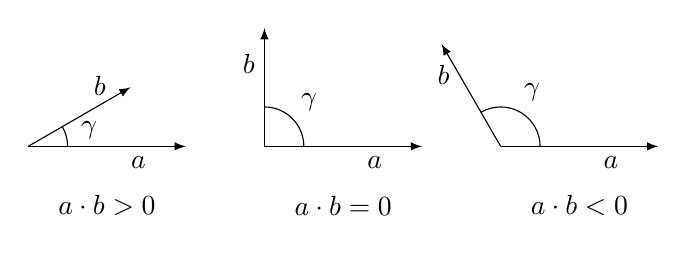
\begin{tikzpicture}
\draw[-latex](0,0)--++(2,0)node[pos=0.7,below]{$\bM{a}$};
\draw[-latex](0,0)--++(30:1.5)node[pos=0.7,above]{$\bM{b}$};
\draw([shift={(0:0.5)}]0,0) arc (0:30:0.5);
\draw(15:0.8) node{$\gamma$};
\draw(1,-0.75)node{$\bM{a}\cdot \bM{b} > 0$};
%
\draw[-latex](3,0)--++(2,0)node[pos=0.7,below]{$\bM{a}$};
\draw[-latex](3,0)--++(90:1.5)node[pos=0.7,left]{$\bM{b}$};
\draw([shift={(0:0.5)}]3,0) arc (0:90:0.5);
\draw(3,0)++(45:0.8) node{$\gamma$};
\draw(4,-0.75)node{$\bM{a}\cdot \bM{b} = 0$};
%
\draw[-latex](6,0)--++(2,0)node[pos=0.7,below]{$\bM{a}$};
\draw[-latex](6,0)--++(120:1.5)node[pos=0.7,left]{$\bM{b}$};
\draw([shift={(0:0.5)}]6,0) arc (0:120:0.5);
\draw(6,0)++(60:0.8) node{$\gamma$};
\draw(7,-0.75)node{$\bM{a}\cdot \bM{b} < 0$};
\end{tikzpicture}
\caption{سمتیات کے مابین زاویہ۔}
\label{شکل_الجبرا_سمتیات_زاویہ}
\end{figure}

اندرونی ضرب کو \اصطلاح{ضرب نقطہ}\فرہنگ{ضرب!نقطہ}\فرہنگ{نقطہ!ضرب}\حاشیہب{dot product}\فرہنگ{dot product} بھی کہتے ہیں۔اندرونی ضرب کا حاصل غیر سمتی (حقیقی عدد) ہوتا ہے اور یوں اندرونی ضرب کو  \اصطلاح{غیر سمتی ضرب}\فرہنگ{غیر سمتی!ضرب}\فرہنگ{ضرب!غیر سمتی}\حاشیہب{scalar product}\فرہنگ{scalar product} بھی کہتے ہیں۔ چونکہ مساوات \حوالہ{مساوات_الجبرا_اندرونی_ضرب} میں \عددی{\cos \gamma} کی قیمت مثبت، صفر یا منفی ہو سکتی ہے (شکل \حوالہ{شکل_الجبرا_سمتیات_زاویہ}) لہٰذا اندرونی ضرب کی قیمت بھی مثبت، صفر یا منفی ہو سکتی ہے۔ زاویہ \عددی{0} تا \عددی{\pi} کے درمیان صرف \عددی{\gamma=\tfrac{\pi}{2}} پر \عددی{\cos \gamma=0} ہو گا جس سے درج ذیل اہم نتیجہ حاصل ہوتا ہے۔

%===================
\ابتدا{مسئلہ}\شناخت{مسئلہ_الجبرا_قائمیت}\quad \اصطلاح{قائمیت}\فرہنگ{قائمیت}\حاشیہب{orthogonality}\فرہنگ{orthogonality}\\
دو عدد غیر صفر سمتیات آپس میں صرف اور صرف اس صورت قائم الزاویہ (\ترچھا{عمودی}) ہوں گے جب ان کا اندرونی ضرب صرف کے برابر ہو۔
\انتہا{مسئلہ}
%=============================

مساوات \حوالہ{مساوات_الجبرا_اندرونی_ضرب} میں \عددی{\bM{b}=\bM{a}} پر کرنے سے \عددی{\bM{a}\cdot\bM{a}=\abs{\bM{a}}^2} حاصل ہوتا ہے اور یوں سمتیہ کی لمبائی (اقلیدسی معیار) کو اندرونی ضرب سے حاصل کیا جا سکتا ہے۔
\begin{align}\label{مساوات_الجبرا_مثبتیت}
\abs{\bM{a}}=\sqrt{\bM{a}\cdot \bM{a}}\quad \quad (\ge 0)
\end{align}
درج بالا اور مساوات \حوالہ{مساوات_الجبرا_اندرونی_ضرب} سے درج ذیل لکھا جا سکتا ہے۔
\begin{align}\label{مساوات_الجبرا_سمتیات_مابین_زاویہ}
\cos \gamma=\frac{\bM{a}\cdot \bM{b}}{\abs{\bM{a}}\abs{\bM{b}}}=\frac{\bM{a}\cdot \bM{b}}{\sqrt{\bM{a}\cdot \bM{a}}\sqrt{\bM{b}\cdot \bM{b}}}
\end{align}
اندرونی ضرب کی تعریف سے درج ذیل خصوصیات اخذ کئے جا سکتے ہیں۔
\begin{gather}
\begin{aligned}\label{مساوات_الجبرا_قواعد_سمتیات_الف}
\text{(الف)}\quad  &[q_1\bM{a}+q_2\bM{b}]\cdot \bM{c}=q_1\bM{a}\cdot \bM{c}+q_2\bM{b}\cdot\bM{c}\quad \text{(خطیت)}\\
\text{(ب)}\quad &\bM{a}\cdot\bM{b}=\bM{b}\cdot \bM{a}\quad \text{(تشاکل)}\\
\text{(پ)}\quad &\left. \begin{array}{ll}
\bM{a}\cdot \bM{a}\ge 0\\
\bM{a}\cdot \bM{a}=0\,\,\text{اگر}\,\, \bM{a}=\bM{0}
\end{array}
\right \}\text{\RL{یقینی مثبت}}
\end{aligned}
\end{gather}

یوں ضرب نقطہ \اصطلاح{استبدالی}\فرہنگ{استبدالی} اور سمتیات کی جمع کے لئے  جزئیتی تقسیمی ہے۔ مساوات \حوالہ{مساوات_الجبرا_قواعد_سمتیات_الف} میں \عددی{q_1=1} اور \عددی{q_2=1} لینے سے درج ذیل ملتا ہے۔
\begin{align}
(\bM{a}+\bM{b})\cdot \bM{c}=\bM{a}\cdot\bM{c}+\bM{b}\cdot \bM{c}\quad \text{\RL{(جزئیتی تقسیم)}}
\end{align}
مساوات \حوالہ{مساوات_الجبرا_اندرونی_ضرب} اور \عددی{\cos \gamma \le 1} سے درج ذیل \اصطلاح{شوارز عدم مساوات}\فرہنگ{شوارز عدم مساوات}\حاشیہب{Schwarz inequality}\فرہنگ{Schwarz inequality}\حاشیہد{جرمن ریاضی دان ہرمن امندس شوارز [1843-1921]} ملتی ہے۔
\begin{align}\label{مساوات_الجبرا_شوارز_عدم_مساوات}
\abs{\bM{a}\cdot\bM{b}}\le \abs{\bM{a}}\abs{\bM{b}}\quad \quad \text{\RL{(شوارز عدم مساوات)}}
\end{align}
درج بالا اور مساوات \حوالہ{مساوات_الجبرا_مثبتیت} استعمال کرتے ہوئے آپ درج ذیل ثابت کر سکتے ہیں۔
\begin{align}
\abs{\bM{a}+\bM{b}}\le \abs{\bM{a}}+\abs{\bM{b}}\quad \quad \text{\RL{(تکونی عدم مساوات)}}
\end{align} 
مساوات \حوالہ{مساوات_الجبرا_مثبتیت} کی مدد سے 
\begin{align*}
\abs{\bM{a}+\bM{b}}^2&=(\bM{a}+\bM{b})\cdot(\bM{a}+\bM{b})=\bM{a}\cdot\bM{a}+\bM{a}\cdot\bM{b}+\bM{b}\cdot\bM{a}+\bM{b}\cdot\bM{b}\\
\abs{\bM{a}-\bM{b}}^2&=(\bM{a}-\bM{b})\cdot(\bM{a}-\bM{b})=\bM{a}\cdot\bM{a}-\bM{a}\cdot\bM{b}-\bM{b}\cdot\bM{a}+\bM{b}\cdot\bM{b}
\end{align*}
لکھ کر دونوں مساوات  جمع کرنے سے درج ذیل ملتا ہے۔
\begin{align}\label{مساوات_الجبرا_متوازی_الاضلاع}
\abs{\bM{a}+\bM{b}}^2+\abs{\bM{a}-\bM{b}}^2=2(\abs{\bM{a}}^2+\abs{\bM{b}}^2)\quad\quad  \text{\RL{(متوازی الاضلاع مساوات)}}
\end{align}
سمتیات کو اجزاء کی صورت  میں لکھ  کر
\begin{align*}
\bM{a}=a_1\bM{i}+a_2\bM{j}+a_3\bM{k},\quad \bM{b}=b_1\bM{i}+b_2\bM{j}+b_3\bM{k}
\end{align*}
ان کا غیر سمتی ضرب معلوم کرتے ہیں۔
\begin{multline*}
\bM{a}\cdot \bM{b}=(a_1\bM{i}+a_2\bM{j}+a_3\bM{k})\cdot (b_1\bM{i}+b_2\bM{j}+b_3\bM{k})\\
=a_1b_1\bM{i}\cdot \bM{i}+a_1b_2\bM{i}\cdot \bM{j}+a_1b_3\bM{i}\cdot \bM{k}+a_2b_1\bM{j}\cdot \bM{i}+a_2b_2\bM{j}\cdot \bM{j}+a_2b_3\bM{j}\cdot \bM{k}\\
+a_3b_1\bM{k}\cdot \bM{i}+a_3b_2\bM{k}\cdot \bM{j}+a_3b_3\bM{k}\cdot \bM{k}
\end{multline*}
اب چونکہ \عددی{\bM{i}} اور \عددی{\bM{j}} آپس میں قائمہ الزاویہ ہیں لہٰذا مساوات \حوالہ{مساوات_الجبرا_اندرونی_ضرب} میں \عددی{\gamma=\tfrac{\pi}{2}} ہو گا اور یوں \عددی{\bM{i}\cdot \bM{j}=0} ہو گا۔اسی طرح چونکہ \عددی{\bM{i}} اور \عددی{\bM{i}} ایک ہی سمت میں ہیں  لہٰذا مساوات \حوالہ{مساوات_الجبرا_اندرونی_ضرب} میں \عددی{\gamma=0} ہو گا اور یوں \عددی{\bM{i}\cdot \bM{i}=1} ہو گا۔اسی عمل سے آپ درج ذیل  غیر سمتی ضرب کے تعلقات لکھ سکتے ہیں جنہیں درج بالا میں
\begin{align}
\bM{i}\cdot\bM{i}&=1,\quad \bM{j}\cdot\bM{j}=1,\quad \bM{k}\cdot\bM{k}=1\\
\bM{i}\cdot\bM{j}&=0,\quad \bM{j}\cdot\bM{k}=0,\quad \bM{k}\cdot\bM{i}=0
\end{align}
پر پر کرتے ہوئے درج ذیل ملتا ہے۔
\begin{align}\label{مساوات_الجبرا_غیر_سمتی_ضرب_اجزاء}
\bM{a}\cdot \bM{b}=a_1b_1+a_2b_2+a_3b_3
\end{align}

اگر \عددی{\bM{a}} اور \عددی{\bM{b}\, (\ne \bM{0})}  سمتیات کے مابین زاویہ \عددی{\gamma} ہو تب درج ذیل حقیقی عدد
\begin{align*}
p=\abs{\bM{a}}\cos \gamma
\end{align*}
\عددی{\bM{b}} کی سمت میں \عددی{\bM{a}} کا \اصطلاح{جزو} یا \اصطلاح{عمودی سایہ}\فرہنگ{عمودی سایہ}\حاشیہب{projection}\فرہنگ{projection} ہو گا۔اگر \عددی{\bM{a}=\bM{0}} ہو تب \عددی{\gamma} غیر معین (بے معنی) ہو گا اور ہم \عددی{p=0} لیں گے۔

یوں \عددی{\bM{b}} کی سمت میں خط \عددی{l} پر \عددی{\bM{a}} کے عمودی سائے کی لمبائی \عددی{\abs{p}} ہو گی۔ \عددی{p} کی قیمت مثبت، صفر یا منفی ہو سکتی ہے (شکل \حوالہ{شکل_الجبرا_عمودی_عکس})۔
\begin{figure}
\centering
\begin{tikzpicture}
\pgfmathsetmacro{\ang}{30}
\pgfmathsetmacro{\a}{1.25}
\pgfmathsetmacro{\aa}{\a*cos(\ang)}
\draw(-0.5,0)node[left]{$l$}--(1.5,0);
\draw[-latex](0,0)--(0.75,0)node[below,pos=0.5]{$\bM{b}$};
\draw[-latex](0,0)--(\ang:\a)node[pos=0.5,above]{$\bM{a}$}coordinate(kT);
\draw[dashed] (kT)--(\aa,0);
\draw([shift={(0:0.3)}]0,0) arc (0:\ang:0.3);
\draw(\ang/2:0.7)node{$\gamma$};
\draw [decorate,decoration={brace,amplitude=5pt},xshift=0,yshift=-3pt](\aa,-0.3)--(0,-0.3)node [black,midway,xshift=0,yshift=-0.5cm] { $\substack{p\\(p>0)}$};
%
\begin{scope}[xshift=-3cm]
\pgfmathsetmacro{\ang}{30}
\pgfmathsetmacro{\a}{1.25}
\pgfmathsetmacro{\aa}{\a*cos(\ang)}
\draw(-1,0)node[left]{$l$}--(1.5,0);
\draw[-latex](0,0)--(0.75,0)node[below]{$\bM{b}$};
\draw[-latex](0,0)--(90:\a)node[pos=0.75,left]{$\bM{a}$}coordinate(kT);
\draw([shift={(0:0.3)}]0,0) arc (0:90:0.3);
\draw(45:0.7)node{$\gamma$};
\draw(0,-1)node{$\substack{\\ (p=0)}$};
\end{scope}
%
\begin{scope}[xshift=-7cm]
\pgfmathsetmacro{\ang}{30}
\pgfmathsetmacro{\a}{1.25}
\pgfmathsetmacro{\aa}{\a*cos(\ang)}
\draw(-1.5,0)node[left]{$l$}--(1.5,0);
\draw[-latex](0,0)--(0.75,0)node[below,pos=0.5]{$\bM{b}$};
\draw[-latex](0,0)--(180-\ang:\a)node[pos=0.5,above]{$\bM{a}$}coordinate(kT);
\draw[dashed] (kT)--(-\aa,0);
\draw([shift={(0:0.3)}]0,0) arc (0:180-\ang:0.3);
\draw(90-\ang/2:0.7)node{$\gamma$};
\draw [decorate,decoration={brace,amplitude=5pt},xshift=0,yshift=-3pt](0,-0.3)--(-\aa,-0.3)node [black,midway,xshift=0,yshift=-0.5cm] { $\substack{p\\(p<0)}$};
\end{scope}
\end{tikzpicture}
\caption{\عددی{\bM{b}} کی سمتی میں \عددی{\bM{a}} کا جزو۔}
\label{شکل_الجبرا_عمودی_عکس}
\end{figure} 

یوں کارتیسی نظام کے اکائی سمتیات \عددی{\bM{i}}، \عددی{\bM{j}} اور \عددی{\bM{k}} کی سمت میں سمتیہ \عددی{\bM{a}=a_1\bM{i}+a_2\bM{j}+a_3\bM{k}} کے اجزاء بالترتیب \عددی{a_1}، \عددی{a_2} اور \عددی{a_3} ہوں گے۔

مساوات \حوالہ{مساوات_الجبرا_سمتیات_مابین_زاویہ} کی مدد سے درج ذیل ہو گا
\begin{align}\label{مساوات_الجبرا_عمودی_سایہ_الف}
p=\bM{a}\cos \gamma=\frac{\bM{a}\cdot\bM{b}}{\abs{\bM{b}}} \quad \quad (\bM{b}\ne \bM{0})
\end{align}
اور اگر \عددی{\bM{b}} اکائی سمتیہ ہو تب اس سے درج ذیل ملتا ہے۔
\begin{align}\label{مساوات_الجبرا_عمودی_سایہ_ب}
p=\bM{a}\cdot\bM{b}
\end{align}
%==================
\ابتدا{مثال}\شناخت{مثال_الجبرا_قوت_کام}\quad قوت اور کام\\
فرض کریں کہ قوت \عددی{\bM{a}} کسی چیز کو اپنی جگہ سے ہٹا کر سمتی فاصلہ \عددی{\bM{d}} منتقل کرتا ہے۔\عددی{\bM{d}} کی سمت میں قوت کا جزو ضرب \عددی{\abs{\bM{d}}} کام \عددی{W} کی تعریف ہے یعنی
\begin{align}
W=\abs{a}\abs{d}\cos \alpha=\bM{a}\cdot \bM{b}
\end{align} 
جہاں \عددی{\bM{a}} اور \عددی{\bM{d}} کے درمیان زاویہ \عددی{\alpha} ہے۔ (شکل \حوالہ{شکل_مثال_الجبرا_قوت_کام})
\begin{figure}
\centering
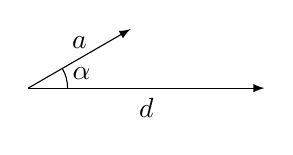
\begin{tikzpicture}
\draw[-latex](0,0)--++(3,0)node[pos=0.5,below]{$\bM{d}$};
\draw[-latex](0,0)--++(30:1.5)node[pos=0.5,above]{$\bM{a}$};
\draw([shift={(0:0.5)}]0,0) arc (0:30:0.5);
\draw(15:0.7)node{$\alpha$};
\end{tikzpicture}
\caption{قوت اور کام (مثال \حوالہ{مثال_الجبرا_قوت_کام})}
\label{شکل_مثال_الجبرا_قوت_کام}
\end{figure}

آپ دیکھ سکتے ہیں کہ \عددی{\bM{a}} کی سمت میں \عددی{\bM{d}} کا جزو ضرب \عددی{\abs{\bM{a}}} بھی کام کی تعریف ہے۔
\انتہا{مثال}
%====================
کارتیسی نظام کی \عددی{xy} سطح پر  کسی بھی نقطے کا \اصطلاح{ہٹاو سمتیہ} \عددی{\bM{r}=x\bM{i}+y\bM{j}}   لکھا جاتا ہے۔\عددی{x=a_1} اور \عددی{y=a_2} کی صورت میں یہ سمتیہ \عددی{\bM{r}_a=a_1\bM{i}+a_2\bM{j}} صورت اختیار کرتا ہے جو کارتیسی نظام کی مرکز سے نقطہ \عددی{N(a_1,a_2)} کی ہٹاو ظاہر کرے گا (شکل \حوالہ{شکل_سیدھے_خط_کی_عمومی_مساوات}-الف)۔

شکل \حوالہ{شکل_سیدھے_خط_کی_عمومی_مساوات}-الف میں نقطہ دار لکیر دکھائی گئی ہے جو \عددی{\bM{r}_a} کے عمودی ہے۔اگر \عددی{x} اور \عددی{y} کو اس نقطہ دار لکیر پر رہنے پر پابند کیا جائے تب \عددی{\bM{r}} اور \عددی{\bM{r}_a} آپس میں قائمہ الزاویہ ہوں گے۔شکل \حوالہ{شکل_سیدھے_خط_کی_عمومی_مساوات}-ب میں ایسا ہی کیا گیا ہے۔یوں شکل-ب میں مسئلہ \حوالہ{مسئلہ_الجبرا_قائمیت} کے تحت درج ذیل ہو گا۔
\begin{align}\label{مساوات_الجبرا_سیدھا_خط_اندرونی_ضرب_الف}
\bM{r}\cdot \bM{r}_a=0\quad \implies \quad  (x\bM{i}+y\bM{j})\cdot(a_1\bM{i}+a_2\bM{j})=a_1x+a_2y=0
\end{align}
 درج بالا مساوات (\عددی{a_1x+a_2y=0}) میں \عددی{x} اور \عددی{y} نقطہ دار خط پر رہتے ہیں لہٰذا یہ نقطہ دار خط کی مساوات ہے۔
\begin{figure}
\centering
\begin{tikzpicture}
%axis
\draw(-1,0)--(2,0)node[below]{$x$};
\draw(0,-0.5)--(0,2)node[left]{$y$};
%lines
\draw[-latex](0,0)--++(0.5,1.5)node[pos=0.9,right]{$\bM{r}$}node[ocirc]{}node[above]{$(x,y)$};
\draw[-latex](0,0)--++(1,0.5)node[pos=0.6,above]{$\bM{r}_a$}node[ocirc]{}node[right]{$N(a_1,a_2)$};
\draw[dashed](0,0)++(90+26.565:-0.5)--++(90+26.565:2);
\draw(0,0)node[ocirc]{};
%
\draw(1,-1)node{(الف)};
\begin{scope}[xshift=-4cm]
%axis
%axis
\draw(-1,0)--(1.2,0)node[below]{$x$};
\draw(0,-0.5)--(0,2)node[left]{$y$};
%lines
\draw[dashed](0,0)++(90+26.565:-0.5)--++(90+26.565:2);
\draw[-latex](0,0)--++(1,0.5)node[pos=0.6,above]{$\bM{r}_a$}node[ocirc]{}node[right]{$N(a_1,a_2)$};
\draw[-latex](0,0)--++(90+26.565:1)node[pos=0.5,left]{$\bM{r}$}node[ocirc]{}node[left]{$(x,y)$};
\draw(0,0)node[ocirc]{};
\draw(1,-1)node{(ب)};
\end{scope}
\end{tikzpicture}
\caption{سیدھے خط کی مساوات۔}
\label{شکل_سیدھے_خط_کی_عمومی_مساوات}
\end{figure}

آپ نے دیکھا کہ سیدھے خط کی مساوات دو سمتیات کی اندرونی ضرب \عددی{\bM{r}\cdot \bM{r}_a=0} کی صورت میں لکھی جا سکتی ہے جہاں \عددی{\bM{r}_a} ایسا ہٹاو سمتیہ ہے جو اس سیدھے خط کے ساتھ قائمہ الزاویہ ہو۔

 ہم شکل \حوالہ{شکل_الجبرا_قائمہ_الزاویہ_خطوط}-الف میں نقطہ \عددی{N} سے گزرتے ہوئے ایسے خط \عددی{L_2} کی مساوات جاننا چاہتے ہیں جو \عددی{L_1} کے  قائمہ الزاویہ ہو۔\عددی{L_1} کی مساوات ہمیں معلوم  ہے۔

کارتیسی نظام میں \عددی{xy} سطح پر کسی بھی سیدھے خط کو \عددی{y=mx+c} لکھا جا سکتا ہے۔اس مساوات میں ڈھلوان \عددی{m} کو  \عددی{\tfrac{a_2}{a_1}}  لکھتے ہوئے \عددی{a_1x+a_2y=ca_1=c'} حاصل ہوتا ہے۔ ایسا ایک خط \عددی{L_1}، شکل \حوالہ{شکل_الجبرا_قائمہ_الزاویہ_خطوط}-الف میں دکھایا گیا ہے۔اس مساوات میں \عددی{c=0} پر کرنے سے خط \عددی{L_1^*} حاصل ہو گا جو کارتیسی نظام کے مرکز \عددی{(0,0)} سے گزرتا ہے جس کو شکل \حوالہ{شکل_الجبرا_قائمہ_الزاویہ_خطوط}-ب میں  دکھایا گیا ہے۔خط \عددی{L_1} اور \عددی{L_1^*} کی ایک جیسی ڈھلوان ہے یعنی یہ آپس میں متوازی ہیں۔ہم \عددی{L_2}  کو بھی اسی طرح مرکز پر منتقل کرتے ہوئے \عددی{L_2^*} حاصل کرتے ہیں۔اب اگر \عددی{L_1} اور \عددی{L_2} قائمہ الزاویہ ہوں تب \عددی{L_1^*} اور \عددی{L_2^*} بھی قائمہ الزاویہ ہوں گے۔آئیں پہلے \عددی{L_1^*} کی مساوات سے \عددی{L_2^*} کی مساوات حاصل کرتے ہیں۔بعد میں حاصل \عددی{L_2^*} کی مساوات سے \عددی{L_2} کی مساوات حاصل کریں گے۔ 
\begin{figure}
\centering
\begin{tikzpicture}
%axis
\draw(-0.5,0)--(2,0)node[below]{$x$};
\draw(0,-0.5)--(0,2)node[left]{$y$};
\draw(0,0)node[ocirc]{};
%lines
\draw(0,0.5)++(18.43:-0.5)--++(18.43:3)node[right]{$L_1$};
\draw(1,1.5)node[ocirc]{}node[above right]{$N(x_0,y_0)$}++(108.43:0.5)--++(108.43:-2)node[pos=0.8,right]{$L_2$};
%
\draw(1,-1)node{(الف)};
\begin{scope}[xshift=-4cm]
%axis
\draw(-0.5,0)--(2,0)node[below]{$x$};
\draw(0,-0.5)--(0,2)node[left]{$y$};
\draw(0,0)node[ocirc]{};
%lines
\draw(0,0)++(18.43:-0.5)--++(18.43:3)node[right]{$L_1^*$};
\draw(0,0)++(108.43:2)node[left]{$L_2^*$}--++(108.43:-2.5);
\draw(1,-1)node{(ب)};
\end{scope}
\end{tikzpicture}
\caption{قائمہ الزاویہ خطوط۔}
\label{شکل_الجبرا_قائمہ_الزاویہ_خطوط}
\end{figure}

\عددی{L_1^*} کی مساوات \عددی{a_1x+a_2y=0}  کو مساوات \حوالہ{مساوات_الجبرا_سیدھا_خط_اندرونی_ضرب_الف} کی طرح سمتیہ \عددی{\bM{r}=x\bM{i}+y\bM{j}} اور سمتیہ \عددی{\bM{r}_a=a_1\bM{i}+a_2\bM{j}} کی اندرونی ضرب \عددی{\bM{r}\cdot\bM{r}_a=a_1x+a_2y=0}  لکھا جا سکتا ہے۔\عددی{L_2^*} کی مساوات کو بھی اسی طرح \عددی{\bM{r}=x\bM{i}+y\bM{j}} اور سمتیہ \عددی{\bM{r}_b=b_1\bM{i}+b_2\bM{j}} کی اندرونی ضرب
 \عددی{\bM{r}\cdot\bM{r}_b=b_1x+b_2y=0}  لکھا جا سکتا ہے۔

اب \عددی{\bM{r}_a} خط \عددی{L_1} کے عمودی ہے جبکہ \عددی{\bM{r}_b} خط \عددی{L_2} کے عمودی ہے۔یوں اگر \عددی{L_1^*} اور \عددی{L_2^*} قائمہ الزاویہ ہوں تب \عددی{\bM{r}_a} اور \عددی{\bM{r}_b} بھی قائمہ الزاویہ ہوں گے اور یوں مسئلہ  \حوالہ{مسئلہ_الجبرا_قائمیت} کے تحت درج ذیل ہو گا۔
\begin{align*}
\bM{r}_a\cdot \bM{r}_b=(a_1\bM{i}+a_2\bM{j})\cdot(b_1\bM{i}+b_2\bM{j})=a_1b_1+a_2b_2=0,\quad \implies \quad b_2=-\frac{a_1}{a_2}b_1
\end{align*}
یوں \عددی{L_2^*} کی مساوات \عددی{\bM{r}\cdot\bM{r}_b=b_1(x-\tfrac{a_1}{a_2}y)=0} ہو گی جس کو ترتیب دیتے ہوئے درج ذیل لکھا جا سکتا ہے۔
\begin{align}
a_2x-a_1y=0\quad \quad (L_2^*)
\end{align}
 \عددی{L_2^*} کی مساوات کا \عددی{L_1^*} کی مساوات \عددی{(a_1x+a_2y=0)} کے ساتھ موازنہ کریں۔

\عددی{L_2^*} کی مساوات  کو استعمال کرتے ہوئے \عددی{L_2} کی مساوات \عددی{a_2x-a_1y=c'} لکھی جا سکتی ہے۔چونکہ \عددی{L_2} نقطہ \عددی{N} سے گزرتی ہے لہٰذا \عددی{(x_0,y_0)} کو \عددی{L_2} کی مساوات میں پر کرتے ہوئے \عددی{c'=a_2x_0-a_1y_0} حاصل کیا جا سکتا ہے۔یوں \عددی{L_2} کی مساوات مکمل ہوتی ہے۔
%===================

%=====================
\ابتدا{مثال}\شناخت{مثال_الجبرا_قائمہ_الزاویہ_خطوط}\quad سیدھی سطح میں واقع قائمہ الزاویہ سیدھے خطوط\\
کارتیسی نظام کی \عددی{xy}  سطح پر ایک خط \عددی{L_1}  کی مساوات \عددی{x-3y-3=0} ہے۔نقطہ \عددی{N(2,3)} سے گزرتا ایسے خط (\عددی{L_2}) کی مساوات دریافت کریں جو \عددی{L_1} کے عمودی ہو۔

\begin{figure}
\centering
\begin{tikzpicture}
%axis
\draw(-0.5,0)--(2,0)node[below]{$x$};
\draw(0,-0.5)--(0,2)node[left]{$y$};
\draw(0,0)node[ocirc]{};
\foreach \x in {1,2,3}{\draw(\x/2,0)--++(0,-0.1)node[below]{$\x$};}
\foreach \y in {1,2,3}{\draw(0,\y/2)--++(-0.1,0)node[left]{$\y$};}
%lines
\draw(0,0.5)++(18.43:-0.5)--++(18.43:3)node[right]{$L_1$};
\draw(1,1.5)node[ocirc]{}node[left]{$N$}++(108.43:0.5)--++(108.43:-2)node[pos=0.8,right]{$L_2$};
%
\draw(1,-1)node{(الف)};
\begin{scope}[xshift=-4cm]
%axis
\draw(-0.5,0)--(2,0)node[below]{$x$};
\draw(0,-0.5)--(0,2)node[left]{$y$};
\draw(0,0)node[ocirc]{};
\foreach \x in {1,2,3}{\draw(\x/2,0)--++(0,-0.1)node[below]{$\x$};}
\foreach \y in {1,2,3}{\draw(0,\y/2)--++(-0.1,0)node[left]{$\y$};}
%lines
\draw(0,0)++(18.43:-0.5)--++(18.43:3)node[right]{$L_1^*$};
\draw(0,0)++(108.43:2)node[left]{$L_2^*$}--++(108.43:-2.5);
\draw(1,-1)node{(ب)};
\end{scope}
\end{tikzpicture}
\caption{قائمہ الزاویہ خطوط (مثال \حوالہ{مثال_الجبرا_قائمہ_الزاویہ_خطوط})۔}
\label{شکل_مثال_الجبرا_قائمہ_الزاویہ_خطوط}
\end{figure}
حل:شکل \حوالہ{شکل_مثال_الجبرا_قائمہ_الزاویہ_خطوط}-الف میں ان خطوط کو دکھایا گیا ہے۔ \عددی{L_1} کو مرکز پر منتقل کرتے ہوئے  \عددی{L_1^*} حاصل ہو گا جس کی مساوات \عددی{x-3y=0} ہو گی جس کو سمتیات \عددی{\bM{r}=x\bM{i}+y\bM{j}} اور \عددی{\bM{r}_a=\bM{i}-3\bM{j}} کا اندرونی ضرب
 \عددی{\bM{r}\cdot\bM{r}_a=(x\bM{i}+y\bM{j})\cdot (\bM{i}-3\bM{j})=x-3y} لکھا جا سکتا ہے۔مرکز سے گزرتی کسی بھی سیدھے خط کی مساوات کی طرح \عددی{L_2^*} کے خط کی مساوات \عددی{b_1x+b_2y=0} لکھی جا سکتی ہے جس کو سمتیات  \عددی{\bM{r}=x\bM{i}+y\bM{j}} اور 
\عددی{\bM{r}_b=b_1\bM{i}+b_2\bM{j}} کا اندرونی ضرب \عددی{\bM{r}\cdot\bM{r}_b=(x\bM{i}+y\bM{j})\cdot (b_1\bM{i}+b_2\bM{j})=b_1x+b_2y} لکھا جا سکتا ہے۔

چونکہ \عددی{L_1} اور \عددی{L_2} آپس میں عمودی ہیں لہٰذا \عددی{\bM{r}_a} اور \عددی{\bM{r}_b} بھی آپس میں عمودی ہوں گے۔ یوں مسئلہ \حوالہ{مسئلہ_الجبرا_قائمیت} کے تحت  \عددی{(\bM{i}-3\bM{j})\cdot (b_1\bM{i}+b_2\bM{j})=b_1-3b_2=0} ہو گا جس سے \عددی{b_1=3b_2} ملتا ہے۔اس طرح \عددی{L_2^*} کی مساوات \عددی{3b_2x+b_2y=0} یا \عددی{3x+y=0} ہو گی جس سے \عددی{L_2} کی مساوات \عددی{3x+y=c'} لکھی جا سکتی ہے۔ \عددی{L_2} نقطہ \عددی{N(2,3)} سے گزرتا ہے لہٰذا حاصل مساوات میں یہ نقطہ پر کرتے ہوئے \عددی{c'=3(2)+3=9} ملتا ہے جس سے \عددی{L_2} کی مساوات \عددی{3x+y=9} ملتی ہے۔
\انتہا{مثال}
%====================================
\ابتدا{مثال}\شناخت{مثال_الجبرا_سیدھی_سطح_اور_عمودی_سمتیہ}\quad سطح کے ساتھ قائمہ الزاویہ سمتیہ\\
ایک سطح کی مساوات \عددی{2x-4y+6z=3} ہے۔ایسا اکائی سمتیہ دریافت کریں جو اس سطح کے ساتھ قائمہ الزاویہ ہو۔

حل:شکل \حوالہ{شکل_سمتیہ_سطحی_قائمہ_الزاویہ} سے رجوع کریں۔سیدھی سطح کی عمومی مساوات درج ذیل ہے۔
\begin{align}\label{مساوات_الجبرا_سیدھی_سطح_الف}
a_1x+a_2y+a_3z=c
\end{align} 
اس سطح پر کسی بھی نقطے کا ہٹاو سمتیہ \عددی{\bM{r}=x\bM{i}+y\bM{j}+z\bM{k}} ہو گا۔یہاں ہم سمتیہ \عددی{\bM{a}=a_1\bM{i}+a_2\bM{j}+a_3\bM{k}} متعارف کرتے ہوئے  مساوات \حوالہ{مساوات_الجبرا_سیدھی_سطح_الف} کو درج ذیل لکھ سکتے ہیں۔
\begin{align}\label{مساوات_الجبرا_سیدھی_سطح_ب}
\bM{a}\cdot\bM{r}=c
\end{align}
\عددی{\bM{a}} غیر صفر (\عددی{\bM{a} \ne \bM{0}}) ہے اور اس کی سمت میں اکائی سمتیہ \عددی{\bM{n}} درج ذیل ہو گا۔
\begin{align*}
\bM{n}=\frac{\bM{a}}{\abs{\bM{a}}}
\end{align*}
مساوات \حوالہ{مساوات_الجبرا_سیدھی_سطح_ب} کو \عددی{\abs{\bM{a}}} سے تقسیم کرتے ہوئے درج ذیل ملتا ہے۔
\begin{align}
\bM{n}\cdot \bM{r}=p,\quad \quad  p=\frac{c}{\abs{\bM{a}}}
\end{align}
مساوات \حوالہ{مساوات_الجبرا_عمودی_سایہ_ب} کی مدد سے ہم دیکھتے ہیں کہ \عددی{\bM{n}} کی سمت میں \عددی{\bM{r}} کا سایہ \عددی{p} ہے۔

اب \عددی{\abs{p}} غیر متغیر مقدار ہے جبکہ سمتیہ \عددی{\bM{r}} سطح پر کوئی بھی نقطہ ہو سکتا ہے۔شکل کو دیکھ کر ظاہر ہے کہ \عددی{p} صرف اور صرف اس صورت غیر متغیر ہو سکتا ہے جب \عددی{\bM{n}} سطح کا قائمہ الزاویہ سمتیہ ہو۔یوں \عددی{\bM{a}} بھی سطح کا قائمہ الزاویہ سمتیہ ہو گا۔شکل یہ یہ بھی ظاہر ہے کہ مرکز سے سطح کے قریب ترین نقطے کا فاصلہ \عددی{\abs{p}} ہو گا۔
\begin{figure}
\centering
\begin{tikzpicture}
\draw[name path=krect](2,0)--++(150:2.2)--++(60:1)--++(-30:2.2)--++(60:-1);
\path[name path=kr](0,0)--(60:1.5)coordinate(kkA);
\path[name path=kB](0,0)--(30:1.75)coordinate(kkB);
\draw[name intersections={of={krect and kr}}](0,0)--(intersection-1);
\draw[dashed](intersection-1)--(kkA);
\draw[-latex](kkA)--++(60:1)node[right]{$\bM{n}$};
%
\draw[name intersections={of={krect and kB}}](0,0)node[ocirc]{}--(intersection-1)node[pos=0.7,below]{$\bM{r}$};
\draw[dashed,-latex](intersection-1)--(kkB)node[circ]{};
\draw [decorate,decoration={brace,amplitude=5pt},xshift=0,yshift=-3pt](0,0)++(150:0.3)--++(60:1.5)node [black,midway,shift={(150:0.5)}] { $\abs{p}$};
\end{tikzpicture}
\caption{سیدھی سطح کا عمودی سمتیہ۔}
\label{شکل_سمتیہ_سطحی_قائمہ_الزاویہ}
\end{figure}

یوں سطح \عددی{2x-4y+6z=3} کا قائمہ الزاویہ سمتیہ \عددی{2\bM{i}-4\bM{j}+6\bM{k}} ہو گا اور سطح کا مرکز سے فاصلہ
 \عددی{\sqrt{2^2+4^2+6^2}=\sqrt{56}} ہو گا۔سطح کا اکائی قائمہ الزاویہ سمتیہ درج ذیل ہو گا۔
\begin{align*}
\bM{n}=\frac{\bM{a}}{\abs{\bM{a}}}=\frac{2\bM{i}-4\bM{j}+6\bM{k}}{\sqrt{56}}
\end{align*}
چونکہ کسی بھی سطح کے دو اطراف ہوتے ہیں لہٰذا \عددی{-\bM{n}} بھی اس سطح کا اکائی قائمہ الزاویہ سمتیہ ہو گا۔
\انتہا{مثال}
%===================================
\ابتدا{مثال}\شناخت{مثال_سمتیہ_مرکز_سے_فاصلہ}
کارتیسی نظام کے \عددی{xy} سطح پر کسی بھی سیدھے خط \عددی{L} کو \عددی{a_1x+a_2y=c} لکھا جا سکتا ہے۔مرکز سے اس خط کا فاصلہ دریافت کریں۔خط کا قائمہ الزاویہ اکائی سمتیہ دریافت کریں۔
\begin{figure}
\centering
\begin{tikzpicture}
\draw[name path=kL](2,-0.5)--++(120:2)node[left]{$L$}coordinate[pos=0.2](kkA);
\path[name path=kN](0,0)--++(30:1.5);
\draw[name intersections={of={kL and kN}}](0,0)--(intersection-1);
\draw[-latex,gray,dashed](intersection-1)--++(30:0.5)node[right]{$\bM{n}$};
\draw[-latex](0,0)node[ocirc]{}--(kkA)node[circ]{}node[pos=0.5,below]{$\bM{r}$};
\end{tikzpicture}
\caption{سیدھے خط کا مرکز سے فاصلہ مثال \حوالہ{مثال_سمتیہ_مرکز_سے_فاصلہ}۔}
\label{شکل_مثال_سمتیہ_مرکز_سے_فاصلہ}
\end{figure}

حل:شکل \حوالہ{شکل_مثال_سمتیہ_مرکز_سے_فاصلہ} سے رجوع کریں۔کارتیسی نظام کی \عددی{xy} سطح پر کسی بھی نقطے کو \عددی{\bM{r}=x\bM{i}+y\bM{j}} لکھا جا سکتا ہے۔سمتیہ \عددی{\bM{a}=a_1\bM{i}+a_2\bM{j}} متعارف کرتے ہوئے دیے گئے سیدھے خط کی مساوات کو درج ذیل لکھا جا سکتا ہے۔
\begin{align*}
\bM{a}\cdot \bM{r}=c
\end{align*} 
اس مساوات کو \عددی{\abs{\bM{a}}} سے تقسیم کرتے ہوئے درج ذیل ملتا ہے۔
\begin{align*}
\bM{n}\cdot \bM{r}=p,\quad \quad \bM{n}=\frac{\bM{a}}{\abs{\bM{a}}},\, p=\frac{c}{\abs{\bM{a}}}
\end{align*}
اب \عددی{\abs{p}} غیر متغیر مقدار ہے جبکہ سمتیہ \عددی{\bM{r}} خط پر کوئی بھی نقطہ ہو سکتا ہے۔شکل کو دیکھ کر ظاہر ہے کہ \عددی{p} صرف اور صرف اس صورت غیر متغیر ہو سکتا ہے جب \عددی{\bM{n}} سطح کا قائمہ الزاویہ سمتیہ ہو۔یوں \عددی{\bM{a}} بھی سطح کا قائمہ الزاویہ سمتیہ ہو گا۔شکل یہ یہ بھی ظاہر ہے کہ مرکز سے سطح کے قریب ترین نقطے کا فاصلہ \عددی{\abs{p}} ہو گا۔

یوں مرکز سے خط تک قائمہ الزاویہ خط \عددی{\bM{a}=a_1\bM{i}+a_2\bM{j}} اور مرکز سے خط تک کم سے کم فاصلہ \عددی{\abs{p}=\sqrt{a_1^2+a_2^2}} ہو گا۔یوں خط کے اکائی قائمہ الزاویہ سمتیات درج ذیل ہوں گے۔
\begin{align*}
\bM{n}=\mp \left(\frac{a_1\bM{i}+a_2\bM{j}}{\sqrt{a_1^2+a_2^2}}\right)
\end{align*} 
\انتہا{مثال}
%=======================

\حصہء{سوالات}
سوال \حوالہ{سوال_سمتیہ_اندرونی_ضرب_وغیرہ_الف} تا سوال \حوالہ{سوال_سمتیہ_اندرونی_ضرب_وغیرہ_ب} میں \عددی{\bM{a}=2\bM{i}+4\bM{j}+\bM{k}}، \عددی{\bM{b}=3\bM{i}-\bM{k}} اور \عددی{\bM{c}=\bM{i}+2\bM{j}-4\bM{k}} ہیں۔

%============
\ابتدا{سوال}\شناخت{سوال_سمتیہ_اندرونی_ضرب_وغیرہ_الف}\quad
$\bM{a}\cdot \bM{b},\, \bM{b}\cdot\bM{a}$\\

جوابات:\عددی{5}، \عددی{5}
\انتہا{سوال}
%=====================
\ابتدا{سوال}\quad
$\abs{\bM{a}},\, \abs{\bM{b}},\, \abs{\bM{c}}$\\

جوابات:\عددی{\abs{\bM{a}}=\sqrt{21}}، \عددی{\abs{\bM{b}}=\sqrt{10}}، \عددی{\abs{\bM{c}}=\sqrt{21}}
\انتہا{سوال}
%=====================
\ابتدا{سوال}\quad
$(\bM{a}-\bM{b})\cdot \bM{c},\, \bM{c}\cdot\bM{a}-\bM{c}\cdot \bM{b}$\\

جوابات:\عددی{-1}
\انتہا{سوال}
%=====================
\ابتدا{سوال}\quad
$(\bM{b}-\bM{c})\cdot \bM{a},\, (\bM{c}-\bM{b})\cdot \bM{a}$\\

جوابات:\عددی{(\bM{b}-\bM{c})\cdot \bM{a}=-1}، \عددی{(\bM{c}-\bM{b})\cdot \bM{a}=1}
\انتہا{سوال}
%=====================
\ابتدا{سوال}\quad
$\abs{\bM{a}+\bM{b}},\, \abs{\bM{a}-\bM{b}}$\\

جوابات:\عددی{\abs{\bM{a}+\bM{b}}=\sqrt{41}}، \عددی{\sqrt{21}}
\انتہا{سوال}
%=====================
\ابتدا{سوال}\quad
$2\bM{a}\cdot 4\bM{c},\, 5\bM{b}\cdot \bM{a}$\\

جوابات:\عددی{2\bM{a}\cdot 4\bM{c}=40}، \عددی{25}
\انتہا{سوال}
%=====================
\ابتدا{سوال}\شناخت{سوال_سمتیہ_اندرونی_ضرب_وغیرہ_ب}\quad
$\abs{\bM{a}+\bM{c}},\, \abs{\bM{a}}+\abs{\bM{c}}$\\

جوابات:\عددی{\abs{\bM{a}+\bM{c}}=3\sqrt{6}}، \عددی{2\sqrt{21}}
\انتہا{سوال}
%=====================
سوال \حوالہ{سوال_سمتیہ_کام_الف} تا سوال \حوالہ{سوال_سمتیہ_کام_ب} میں ایک چیز کو قوت \عددی{\bM{f}} نقطہ \عددی{A} سے نقطہ \عددی{B} منتقل کرتی ہے۔ قوت کتنا کام کرتا ہے؟ کام کی تعریف \عددی{\bM{f}\cdot \bM{r}_{BA}} ہے۔

%====================
\ابتدا{سوال}\شناخت{سوال_سمتیہ_کام_الف}\quad 
$\bM{f}=\bM{i}+\bM{j}-\bM{k},\, A(0,0,0),\, B(5,0,0)$\\
جواب:\عددی{\SI{5}{\joule}}
\انتہا{سوال}
%====================
\ابتدا{سوال}\quad 
$\bM{f}=2\bM{i}-3\bM{j}+\bM{k},\, A(2,5,0),\, B(0,0,0)$\\
جواب:\عددی{\SI{11}{\joule}}
\انتہا{سوال}
%====================
\ابتدا{سوال}\quad 
$\bM{f}=3\bM{i}+\bM{j}-2\bM{k},\, A(-5,2,1),\, B(2,-3,-6)$\\
جواب:\عددی{\SI{30}{\joule}}
\انتہا{سوال}
%====================
\ابتدا{سوال}\شناخت{سوال_سمتیہ_کام_صفر}\quad 
$\bM{f}=5\bM{i}+2\bM{j}+3\bM{k},\, A(5,5,6),\, B(7,6,2)$\\
جواب:\عددی{\SI{0}{\joule}}
\انتہا{سوال}
%====================
\ابتدا{سوال}\شناخت{سوال_سمتیہ_کام_ب}\quad 
$\bM{f}=2\bM{i}+\bM{j}+3\bM{k},\, A(3,4,2),\, B(4,2,1)$\\
جواب:\عددی{\SI{-3}{\joule}}
\انتہا{سوال}
%====================
\ابتدا{سوال}
سوال \حوالہ{سوال_سمتیہ_کام_صفر} میں کام صفر کیوں ہے؟

جواب:چونکہ قوت اور ہٹاو سمتیہ قائمہ الزاویہ ہیں۔
\انتہا{سوال}
%======================
\ابتدا{سوال}
سوال \حوالہ{سوال_سمتیہ_کام_صفر} میں کام منفی کیوں ہے؟

جواب:چونکہ قوت اور ہٹاو سمتیہ آپس میں الٹ رخ ہیں۔
\انتہا{سوال}
%======================
\ابتدا{سوال}
سمتیہ \عددی{4\bM{i}-2\bM{j}+c\bM{k}} میں \عددی{c} کی قیمت کیا ہونے سے یہ  سمتیہ \عددی{2\bM{i}+3\bM{j}-3\bM{k}} کے عمودی ہو گا۔

جواب:\عددی{2}
\انتہا{سوال}
%======================
\ابتدا{سوال}
\عددی{xy} سطح میں \عددی{4\bM{i}-2\bM{j}} کا عمودی اکائی سمتیہ دریافت کریں۔

جواب:\عددی{\tfrac{\bM{i}+2\bM{j}}{\sqrt{5}}} اور \عددی{\tfrac{-\bM{i}-2\bM{j}}{\sqrt{5}}}
\انتہا{سوال}
%=========================
\ابتدا{سوال}
ایک چیز کو قوت \عددی{\bM{f}_1} اور قوت \عددی{\bM{f}_2} مل کر نقطہ \عددی{A} سے نقطہ \عددی{B} منتقل کرتی ہے۔ثابت کریں کہ کل کام دونوں قوتوں کے کاموں کا مجموعہ ہو گا۔
\انتہا{سوال}
%=======================
\ابتدا{سوال}
سمتیات استعمال کرتے ہوئے ثابت کریں کہ اگر مستطیل کے وتر آپس میں عمودی ہوں تب یہ مستطیل دراصل میں چکور ہو گا۔
\انتہا{سوال}
%=====================
\ابتدا{سوال}
سمتیات استعمال کرتے ہوئے ثابت کریں کہ مکعب کے بالکل الٹ کونوں کو ملاتے ہوئے وتر آپس میں عمودی ہوں گے۔
\انتہا{سوال}
%====================
\ابتدا{سوال}
ثابت کریں کہ سطح \عددی{7x+y+3z=22} اور سطح \عددی{x-y-2z=-5} قائمہ الزاویہ ہیں۔

جواب:ان کے عمودی سمتیات \عددی{7\bM{i}+\bM{j}+3\bM{k}} اور \عددی{\bM{i}-\bM{j}-2\bM{k}} کا اندرونی ضرب صفر ہے لہٰذا یہ آپس میں عمودی ہیں اور یوں  سطحیں بھی عمودی ہوں گی۔
\انتہا{سوال}
%=======================
\ابتدا{سوال}
سطح \عددی{3x-2y+z=-2} اور \عددی{x-4y-2z=3} کے مابین زاویہ دریافت کریں۔

جواب:\عددی{1.0182} ریڈیئن یعنی \عددی{58.33^{\circ}}
\انتہا{سوال}
%====================
\ابتدا{سوال}
تکون کے تین کونے \عددی{A(2,-4,6)}، \عددی{B(5,2,4)} اور \عددی{C(-2,-1,-4)} ہیں۔ اس تکون کے زاویے دریافت کریں۔

جوابات:\عددی{74.61^{\circ}}، \عددی{42.98^{\circ}}، \عددی{62.4^{\circ}}
\انتہا{سوال}
%===================
سوال \حوالہ{سوال_سمتیہ_زاویہ_الف} تا سوال \حوالہ{سوال_سمتیہ_زاویہ_ب} میں \عددی{\bM{a}=2\bM{i}-4\bM{j}+\bM{k}}، \عددی{\bM{b}=\bM{i}+\bM{j}} اور \عددی{\bM{c}=\bM{j}+2\bM{k}} ہیں۔دی گئی جوڑی سمتیات کے مابین زاویہ دریافت کریں۔

%===================
\ابتدا{سوال}\شناخت{سوال_سمتیہ_زاویہ_الف}\quad
$\bM{a}, \, \bM{b}$\\
جواب:\عددی{107.98^{\circ}}
\انتہا{سوال}
%======================
\ابتدا{سوال}\quad
$\bM{a}-\bM{b}, \, \bM{b}+\bM{c}$\\
جواب:\عددی{116.68^{\circ}}
\انتہا{سوال}
%======================
\ابتدا{سوال}\شناخت{سوال_سمتیہ_زاویہ_ب}\quad
$\bM{a}, \, 2\bM{a}-3\bM{b}+4\bM{c}$\\
جواب:\عددی{44.54^{\circ}}
\انتہا{سوال}
%======================
درج ذیل چار سوالات میں \عددی{\bM{a}} کی سمت میں \عددی{\bM{b}} کا جزو دریافت کریں۔

%=================
\ابتدا{سوال}\quad
$\bM{a}=\bM{i}+\bM{j}+\bM{k},\, \bM{b}=3\bM{i}-7\bM{k}$\\
جواب:\عددی{\bM{a}} کی سمت میں \عددی{\bM{b}} کی لمبائی \عددی{\bM{a}\cdot\bM{b}=-4} ہے۔اب چونکہ \عددی{\bM{a}} کی سمت میں اکائی سمتیہ
 \عددی{\tfrac{\bM{i}+\bM{j}+\bM{k}}{\sqrt{3}}} ہے لہٰذا \عددی{\bM{a}} کی سمت میں \عددی{\bM{b}} کا جزو
 \عددی{\tfrac{-4}{\sqrt{3}}(\bM{i}+\bM{j}+\bM{k})} ہو گا۔
\انتہا{سوال}
%=================
\ابتدا{سوال}\quad
$\bM{a}=\bM{i}+\bM{j}-2\bM{k},\, \bM{b}=2\bM{i}+\bM{j}-2\bM{k}$\\
جواب:\عددی{-1.22\bM{i}+1.22\bM{j}-2.45\bM{k}}
\انتہا{سوال}
%==================
\ابتدا{سوال}\quad
$\bM{a}=3\bM{j}+4\bM{k},\, \bM{b}=3\bM{i}+4\bM{j}$\\
جواب:\عددی{7.2\bM{j}+9.6\bM{k}}
\انتہا{سوال}
%==================
\ابتدا{سوال}\quad
$\bM{a}=-2\bM{i}+3\bM{j}-4\bM{k},\, \bM{b}=3\bM{i}-4\bM{j}-6\bM{k}$\\
جواب:\عددی{-2.23\bM{i}+3.34\bM{j}-4.46\bM{k}}
\انتہا{سوال}
%==================
\ابتدا{سوال}
ثابت کریں کہ \عددی{\bM{i}+\bM{j}+\bM{k}} تینوں اکائی سمتیات \عددی{\bM{i}}، \عددی{\bM{j}} اور \عددی{\bM{k}} کے ساتھ یکساں زاویہ بناتا ہے۔

جواب:\عددی{54.73^{\circ}}
\انتہا{سوال}
%======================

\حصہ{اندرونی ضرب فضا}
تین بعدی فضا میں، مجموعہ سمتیات اور سمتیہ کا غیر سمتی کے ساتھ ضرب کے بنیادی قواعد استعمال کرتے ہوئے حصہ \حوالہ{حصہ_الجبرا_سمتیات_فضا_تابعیت} میں سمتی فضا کا تصور متعارف کرایا گیا۔ ہم اسی طرح اندرونی ضرب  (حصہ \حوالہ{حصہ_سمتیہ_اندرونی_ضرب_فضا}) کو استعمال کرتے ہوئے \اصطلاح{حقیقی اندرونی ضرب فضا}\فرہنگ{فضا!حقیقی اندرونی ضرب}\حاشیہب{real inner product space}\فرہنگ{space!real inner product} کا تصور حاصل کر سکتے ہیں۔ ایسا حقیقی سمتی فضا جس میں اندرونی ضرب مساوات \حوالہ{مساوات_الجبرا_قواعد_سمتیات_الف} کے شرائط پر پورا اترتا ہو \اصطلاح{حقیقی اندرونی ضرب فضا} کہلاتا ہے۔  
%========================
\ابتدا{تعریف}\quad اندرونی ضرب فضا\\
ایسی حقیقی سمتی فضا \عددی{V} جو درج ذیل خصوصیت رکھتی ہو \اصطلاح{حقیقی اندرونی ضرب فضا} کہلاتی ہے۔  

\عددی{V} میں ہر دو عدد سمتیات \عددی{\bM{a}} اور \عددی{\bM{b}} کے ساتھ ایک ایسا حقیقی عدد  وابستہ ہے، جس کو \عددی{(\bM{a},\bM{b})} سے ظاہر کیا جاتا ہے اور جو \عددی{\bM{a}} اور \عددی{\bM{b}} کا اندرونی ضرب کہلاتا ہے، کہ درج ذیل مسلمات پورا ہوتے ہوں۔
\begin{itemize}
\item{(الف)}
کسی بھی غیر سمتیات \عددی{q_1} اور \عددی{q_2} اور \عددی{V} میں تمام سمتیات \عددی{\bM{a}}، \عددی{\bM{b}}، \عددی{\bM{c}} کے لئے درج ذیل ہو گا۔
\begin{align*}
\text{(الف)}\quad (q_1\bM{a}+q_2\bM{b},\bM{c})=q_1(\bM{a},\bM{c})+q_2(\bM{b},\bM{c})\quad \quad (\text{خطیت})
\end{align*}
\item{(ب)}
\عددی{V} میں تمام سمتیات \عددی{\bM{a}} اور \عددی{\bM{b}} کے لئے درج ذیل ہو گا۔
\begin{align*}
(\bM{a},\bM{b})=(\bM{b},\bM{a})\quad \quad (\text{تشاکل})
\end{align*}
\item{(پ)}
\عددی{V} میں ہر \عددی{\bM{a}} کے لئے درج ذیل ہو گا۔
\begin{align*}
\left.
\begin{array}{ll}
(\bM{a},\bM{a})\ge 0\\
(\bM{a},\bM{a})=0 \quad \text{اگر}\quad \bM{a}=\bM{0}
\end{array}
\right\} \text{\RL{یقینی مثبت}}
\end{align*}
\end{itemize} 
\انتہا{تعریف}
%======================
\ابتدا{تعریف}\quad قائمیت\\
اگر اندرونی ضرب فضا \عددی{V} میں دو سمتیات \عددی{\bM{a}} اور \عددی{\bM{b}} کا اندرونی ضرب صفر کے برابر ہو تب یہ سمتیات آپس میں قائم الزاویہ ہوں گے۔
\begin{align*}
(\bM{a},\bM{b})=0\quad \quad (\text{\RL{قائم الزاویہ}})
\end{align*} 
\انتہا{تعریف}
%============================
اندرونی ضرب  کو استعمال کرتے ہوئے ہم اندرونی ضرب فضا \عددی{V} میں ہر \عددی{\bM{a}} کے ساتھ عدد \عددی{\norm{\bM{a}}} وابستہ کرتے ہیں جس کی تعریف درج ذیل ہے
\begin{align*}
\norm{\bM{a}}=\sqrt{(\bM{a},\bM{a})}\quad (\ge 0)
\end{align*}
اور جو \عددی{\bM{a}} کی \اصطلاح{معیار}\فرہنگ{معیار}\حاشیہب{norm}\فرہنگ{norm} کہلاتا ہے۔مساوات \حوالہ{مساوات_الجبرا_مثبتیت} کے ساتھ موازنہ کرنے سے آپ دیکھ سکتے ہیں کہ \اصطلاح{معیار} درحقیقت لمبائی کی عمومی تعریف ہے۔حقیقت میں ضرب نقطہ اور موجودہ  اندرونی ضرب یکساں ہیں یعنی
\begin{align*}
(\bM{a},\bM{b})=\bM{a}\cdot\bM{b}
\end{align*}
اور ہماری موجودہ تعریف کے تحت مساوات \حوالہ{مساوات_الجبرا_مثبتیت} کو درج ذیل لکھا جا سکتا ہے۔
\begin{align*}
\norm{\bM{a}}=\abs{\bM{a}}=\sqrt{(\bM{a},\bM{a})}=\sqrt{\bM{a}\cdot\bM{a}}
\end{align*}
 مسلمات اندرونی ضرب اور معیار کی تعریف سے  مساوات \حوالہ{مساوات_الجبرا_شوارز_عدم_مساوات} تا مساوات \حوالہ{مساوات_الجبرا_متوازی_الاضلاع} اخذ کیے جا سکتے ہیں۔
\begin{align*}
\abs{(\bM{a},\bM{b})}\le \norm{\bM{a}}\norm{\bM{b}} \quad \quad (\text{\RL{(شوارز عدم مساوات)}})
\end{align*}
درج بالا سے درج ذیل لکھا جا سکتا ہے
\begin{align*}
\norm{\bM{a}+\bM{b}}\le \norm{\bM{a}}+\norm{\bM{b}}\quad \quad \text{\RL{تکونی عدم مساوات}}
\end{align*}
اور سادہ الجبرائی حساب سے درج ذیل لکھا جا سکتا ہے۔
\begin{align*}
\norm{\bM{a}+\bM{b}}^2+\norm{\bM{a}-\bM{b}}^2=2(\norm{\bM{a}}^2+\norm{\bM{b}}^2)\quad \quad (\text{\RL{متوازی الاضلاع مساوات}})
\end{align*}
اندرونی ضرب فضا کا تصور عمومی ہے جس کی دو مثالیں (بغیر ثبوت) پیش کرتے ہیں۔پہلی مثال \عددی{n} اجزاء پر مشتمل سمتیات \عددی{\bM{a}=(a_1,\cdots,a_n)} اور \عددی{\bM{b}=(b_1,\cdots,\b_n)} کا اندرونی ضرب ہے جس کی تعریف درج ذیل ہے۔
\begin{align}
(\bM{a},\bM{b})=a_!b_1+a_2b_2+\cdots+a_nb_n
\end{align}
اندرونی ضرب فضا کی دوسری مثال، وقفہ \عددی{\alpha \le x\le \beta} پر  استمراری تفاعل \عددی{f(x)} اور \عددی{g(x)} کی اندرونی ضرب ہے جس  کی تعریف درج ذیل ہے۔
\begin{align}
(f,g)=\int_{\alpha}^{\beta} f(x)g(x)\dif x
\end{align}
%=================
\حصہ{سمتی ضرب}\شناخت{حصہ_سمتیات_سمتی_ضرب}
کئی عملی مسائل سے سمتیات کی ایسی ضرب کی ضرورت پیش ہوتی ہے جس کا حاصل ضرب \عددی{\bM{v}} بھی سمتیہ ہو۔\عددی{\bM{a}} اور \عددی{\bM{b}} سمتیات کا ایسا ضرب جو \اصطلاح{سمتی ضرب}\فرہنگ{سمتی ضرب}\حاشیہب{vector product}\فرہنگ{vector product} یا \اصطلاح{صلیبی ضرب}\فرہنگ{صلیبی ضرب}\حاشیہب{cross product}\فرہنگ{cross product} کہلاتا اور \عددی{\bM{a}\times \bM{b}} لکھا جاتا ہے
\begin{align*}
\bM{v}=\bM{a}\times \bM{b}
\end{align*}
کی تعریف درج ذیل ہے۔
%====================

\ابتدا{تعریف}\شناخت{تعریف_الجبرا_سمتی_ضرب}\quad سمتی ضرب\\
اگر \عددی{\bM{a}} اور \عددی{\bM{b}} کے رخ ایک جیسے یا آپس میں الٹ ہوں اور یا ان سمتیات میں سے ایک (یا دونوں) صفر سمتیہ ہوں تب \عددی{\bM{v}=\bM{a}\times \bM{b}=\bM{0}} ہو گا۔

اس کے علاوہ \عددی{\bM{v}=\bM{a}\times \bM{b}} ایسا سمتیہ ہو گا جس کی لمبائی اس متوازی الاضلاع کے رقبے کے برابر ہو گی جس کے قریبی اطراف \عددی{\bM{a}} اور \عددی{\bM{b}} ہوں اور جس کی سمت \عددی{\bM{a}} اور \عددی{\bM{b}} دونوں کے عمودی ہو گی۔ مزید \عددی{\bM{v}} کی سمت یوں ہو گی کہ \عددی{\bM{a}}، \عددی{\bM{b}} اور \عددی{\bM{v}} (اسی ترتیب سے) دائیں ہاتھ کی ثلاثہ قائمہ سمتیات ہوں (شکل \حوالہ{شکل_تعریف_الجبرا_سمتی_ضرب}-الف)۔
 \begin{figure}
\centering
\begin{subfigure}{0.5\textwidth}
\centering
\begin{tikzpicture}
\draw[-latex](0,0)--++(-40:2)node[pos=0.7,below]{$\bM{a}$}coordinate(kA);
\draw[-latex](0,0)--++(15:1.5)node[pos=0.7,above]{$\bM{b}$}coordinate(kB);
\draw[-latex](0,0)--++(0,1.5)node[left]{$\bM{v}$}coordinate(kC);
\draw[dashed](kA)--++(15:1.5);
\draw[dashed](kB)--++(-40:2);
\draw[gray] (0,0.2)--++(15:0.3)--++(0,-0.2);
\draw[gray] (0,0.2)--++(-40:0.3)--++(0,-0.2);
\end{tikzpicture}
\caption*{(الف) سمتی ضرب}
\end{subfigure}%
\begin{subfigure}{0.5\textwidth}
\centering
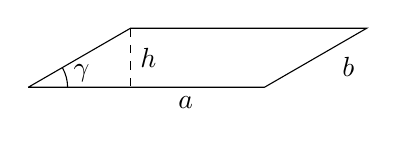
\begin{tikzpicture}
\pgfmathsetmacro{\kh}{1.5*sin(30)};
\draw(0,0)--++(3,0)--++(30:1.5)--++(-3,0)--(0,0);
\draw([shift={(0:0.5)}]0,0) arc (0:30:0.5);
\draw(15:0.7)node{$\gamma$};
\draw(2,0)node[below]{$\abs{\bM{a}}$};
\draw(3,0)++(30:1)node[below right]{$\abs{\bM{b}}$};
\draw[dashed](30:1.5)--++(0,-\kh)node[pos=0.5,right]{$h$}coordinate(kB);
\RightAngle{(30:1.5)}{(kB)}{(0,0)};
\end{tikzpicture}
\caption*{(ب) متوازی الاضلاع کا رقبہ۔}
\end{subfigure}%
\caption{سمتی ضرب کی تعریف}
\label{شکل_تعریف_الجبرا_سمتی_ضرب}
\end{figure}
\انتہا{تعریف}
%========================
 سمتی ضرب کی تعریف میں ثلاثہ قائمہ سمتیات کی بات کرتے ہوئے  دائیں ہاتھ کا ذکر کیا گیا جس کا مطلب ہے کہ  اگر دائیں ہاتھ کا انگوٹھا سمتیہ \عددی{\bM{a}} کی سمت میں اور انگلی شہادت سمتیہ \عددی{\bM{b}} کی سمت میں رکھتے ہوئے  درمیانی انگلی کو ان انگلیوں کے عمودی رکھا جائے تب درمیانی انگلی سمتیہ \عددی{\bM{v}} کی مقام  کو ظاہر کرے گی۔ 

ایسا متوازی الاضلاع (شکل \حوالہ{شکل_تعریف_الجبرا_سمتی_ضرب}-ب) جس کے قریبی اطراف \عددی{\bM{a}} اور \عددی{\bM{b}} ہوں کا رقبہ
 \عددی{h \abs{\bM{a}}=\abs{\bM{a}}\abs{\bM{b}}\sin \gamma} ہو گا جہاں \عددی{\bM{a}} اور \عددی{\bM{b}} کے مابین زاویہ \عددی{\gamma} ہے ۔
\begin{align}\label{مساوات_الجبرا_سمتی_ضرب_رقبہ}
\abs{\bM{v}}=\abs{\bM{a}}\abs{\bM{b}}\sin \gamma
\end{align}

اگر\عددی{\bM{v}=\bM{a}\times\bM{b}} اور \عددی{\bM{w}=\bM{b}\times\bM{a}} ہوں تب سمتی ضرب کی تعریف کے تحت \عددی{\abs{\bM{v}}=\abs{\bM{w}}} ہو گا۔اب  \عددی{\bM{a}}، \عددی{\bM{b}} اور \عددی{\bM{w}} اس صورت دائیں ہاتھ ثلاثہ قائمہ سمتیات ہوں گے جب \عددی{\bM{w}=-\bM{v}} (شکل \حوالہ{شکل_الجبرا_مخالف_تبادل_سمتی_ضرب}) ہو لہٰذا ہم درج ذیل لکھ سکتے ہیں
\begin{align}
\bM{b} \times \bM{a}=-\bM{a}\times \bM{b}
\end{align}
جس کے تحت سمتی ضرب مخالف تبادل ہے۔یوں سمتی ضرب میں اجزاء کی ترتیب نہایت اہم ہے جس کو تبدیل نہیں کیا جا سکتا ہے۔
\begin{figure}
\centering
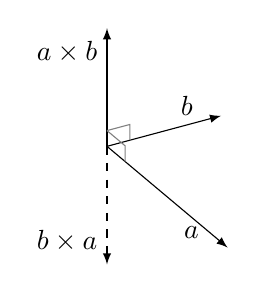
\begin{tikzpicture}
\draw[-latex](0,0)--++(-40:2)node[pos=0.7,below]{$\bM{a}$}coordinate(kA);
\draw[-latex](0,0)--++(15:1.5)node[pos=0.7,above]{$\bM{b}$}coordinate(kB);
\draw[-latex](0,0)--++(0,1.5)node[pos=0.8,left]{$\bM{a}\times \bM{b}$}coordinate(kC);
\draw[-latex,dashed](0,0)--++(0,-1.5)node[pos=0.8,left]{$\bM{b}\times \bM{a}$};
%right angles
\draw[gray] (0,0.2)--++(15:0.3)--++(0,-0.2);
\draw[gray] (0,0.2)--++(-40:0.3)--++(0,-0.2);
\end{tikzpicture}
\caption{سمتی ضرب مخالف تبادل ہے}
\label{شکل_الجبرا_مخالف_تبادل_سمتی_ضرب}
\end{figure}

کسی بھی غیر سمتیہ \عددی{k} کے لئے سمتی ضرب کی تعریف سے درج ذیل لکھا جا سکتا ہے۔
\begin{align}
(k\bM{a})\times \bM{b}=k(\bM{a}\times \bM{b})=\bM{a}\times(k\bM{b})
\end{align}
سمتی جمع کی نقطہ نظر سے سمتی ضرب جزئیتی تقسیمی ہے یعنی:
\begin{gather}
\begin{aligned}\label{مساوت_الجبرا_جزئیتی_تقسیم_برائے_سمتی_ضرب}
\bM{a}\times (\bM{b}+\bM{c})&=(\bM{a}\times \bM{b})+(\bM{a}\times \bM{c})\\
(\bM{a}+\bM{b})\times \bM{c}&=(\bM{a}\times \bM{c})+(\bM{b}\times \bM{c})
\end{aligned}
\end{gather}
درج بالا کا ثبوت اگلے حصے میں پیش کیا جائے گا۔ہم یہاں بتلانا چاہتے ہیں کہ سمتی ضرب قانون تلازم  پر عموماً پورا \موٹا{نہیں} اترتا یعنی:
\begin{align*}
\bM{a}\times (\bM{b}\times \bM{c}) \ne (\bM{a}\times \bM{b})\times \bM{c}
\end{align*}

مساوات \حوالہ{مساوات_الجبرا_اندرونی_ضرب} اور مساوات \حوالہ{مساوات_الجبرا_سمتی_ضرب_رقبہ} سے درج ذیل لکھا جا سکتا ہے۔
\begin{align*}
\abs{\bM{v}}^2=\abs{\bM{a}}^2\abs{\bM{b}}^2\sin^2\gamma=\abs{\bM{a}}^2\abs{\bM{b}}^2(1-\cos^2\gamma)=(\bM{a}\cdot\bM{a})(\bM{b}\cdot\bM{b})-(\bM{a}\cdot\bM{b})^2
\end{align*}
دونوں اطراف کا جذر لیتے ہوئے حاصل سمتی ضرب کی لمبائی کا درج ذیل قلیہ حاصل ہوتا ہے۔
\begin{align}\label{مساوات_الجبرا_سمتی_ضرب_معیار_کی_اہم_مساوات}
\abs{\bM{a}\times \bM{b}}=\sqrt{(\bM{a}\cdot\bM{a})(\bM{b}\cdot\bM{b})-(\bM{a}\cdot\bM{b})^2}
\end{align}
%=============================================
\حصہ{اجزاء کی صورت میں سمتی ضرب}
اس حصے میں ہم سمتی ضرب کے اجزاء کو کارتیسی نظام میں لکھتے ہیں۔یہاں یہ بتلانا ضروری ہے کہ دو قسم کے کارتیسی نظام ممکن ہیں۔پہلا قسم  \اصطلاح{دائیں ہاتھ}\فرہنگ{کارتیسی نظام!دائیں ہاتھ}\فرہنگ{دایاں ہاتھ!کارتیسی نظام}\حاشیہب{right handed}\فرہنگ{right handed} کا نظام کہلاتا ہے۔ دائیں ہاتھ کارتیسی نظام میں محور کی مثبت سمت میں اکائی سمتیات \عددی{\bM{i}}، \عددی{\bM{j}} اور \عددی{\bM{k}} دائیں ہاتھ ثلاثہ قائمہ سمتیات ہوں گے (شکل \حوالہ{شکل_الجبرا_کارتیسی_بایاں_دایاں_نظام}-الف)۔ اگر نظام کے اکائی سمتیات بائیں ہاتھ ثلاثہ قائمہ سمتیات ہوں تب اس کو بایاں ہاتھ کارتیسی نظام کہا جائے گا۔اس کتاب میں دایاں ہاتھ کارتیسی نظام استعمال کیا گیا ہے۔عام استعمال میں بھی دایاں نظام استعمال کیا جاتا ہے۔ 
\begin{figure}
\centering
\begin{subfigure}{0.5\textwidth}
\centering
\begin{tikzpicture}[x={(-0.5cm,-0.5cm)},y={(1cm,0)},z={(0,1cm)}]
%axis
\draw[gray](0,0)--++(2,0,0)node[left]{$x$};
\draw[gray](0,0)--++(0,2,0)node[below]{$y$};
\draw[gray](0,0)--++(0,0,1.5)node[right]{$z$};
%vectors
\draw[-latex](0,0,0)--++(1,0,0)node[pos=0.7,left]{$\bM{i}$};
\draw[-latex](0,0,0)--++(0,1,0)node[below]{$\bM{j}$};
\draw[-latex](0,0,0)--++(0,0,1)node[left]{$\bM{k}$};
\end{tikzpicture}
\caption*{(الف) دایاں ہاتھ کارتیسی نظام}
\end{subfigure}%
\begin{subfigure}{0.5\textwidth}
\centering
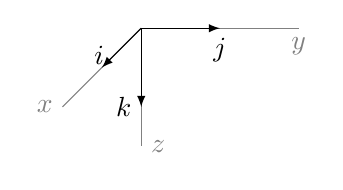
\begin{tikzpicture}[x={(-0.5cm,-0.5cm)},y={(1cm,0)},z={(0,1cm)}]
%axis
\draw[gray](0,0)--++(2,0,0)node[left]{$x$};
\draw[gray](0,0)--++(0,2,0)node[below]{$y$};
\draw[gray](0,0)--++(0,0,-1.5)node[right]{$z$};
%vectors
\draw[-latex](0,0,0)--++(1,0,0)node[pos=0.7,left]{$\bM{i}$};
\draw[-latex](0,0,0)--++(0,1,0)node[below]{$\bM{j}$};
\draw[-latex](0,0,0)--++(0,0,-1)node[left]{$\bM{k}$};
\end{tikzpicture}
\caption*{(ب) بایاں ہاتھ کارتیسی نظام}
\end{subfigure}%
\caption{کارتیسی نظام کے دو اقسام}
\label{شکل_الجبرا_کارتیسی_بایاں_دایاں_نظام}
\end{figure}

اب دائیں یا بائیں ہاتھ کے نظام میں اگر \عددی{\bM{a}} اور \عددی{\bM{b}} کے اجزاء بالترتیب \عددی{a_1}، \عددی{a_2}، \عددی{a_3} اور \عددی{b_1}، \عددی{b_2}، \عددی{b_3} ہوں تب سمتی ضرب 
\begin{align*}
\bM{a}\times \bM{b}
\end{align*}
کے اجزاء کو انہیں کی صورت میں لکھا جا سکتا ہے۔ہمیں صرف اس صورت پر غور کرنا ہے جب \عددی{\bM{v} \ne \bM{0}} ہو۔چونکہ \عددی{\bM{v}} دونوں سمتیات \عددی{\bM{a}} اور \عددی{\bM{b}} کے عمودی ہے لہٰذا مسئلہ \حوالہ{مسئلہ_الجبرا_قائمیت} کے تحت \عددی{\bM{a}\cdot \bM{v}=0} اور \عددی{\bM{b}\cdot \bM{v}=0} ہوں گے لہٰذا مساوات \حوالہ{مساوات_الجبرا_غیر_سمتی_ضرب_اجزاء} کی مدد سے درج ذیل لکھا جا سکتا ہے۔
\begin{gather}
\begin{aligned}\label{مساوات_الجبرا_سمتی_ضرب_اجزاء_کی_صورت_الف}
a_1v_1+a_2v_2+a_3v_3&=0\\
b_1v_1+b_2v_2+b_3v_3&=0
\end{aligned}
\end{gather}
پہلی مساوات کو \عددی{b_3} اور دوسری کو \عددی{a_3} سے ضرب دے کر ان کا فرق حاصل کرتے ہیں۔
\begin{align*}
(a_3b_1-a_1b_3)v_1=(a_2b_3-a_3b_2)v_2
\end{align*}
اسی طرح مساوات \حوالہ{مساوات_الجبرا_سمتی_ضرب_اجزاء_کی_صورت_الف} کی پہلی مساوات کو \عددی{b_1} اور دوسری کو \عددی{a_1} سے ضرب دے کر ان کا فرق  لکھتے ہیں۔ 
\begin{align*}
(a_1b_2-a_2b_1)v_2=(a_3b_1-a_1b_3)v_3
\end{align*}
آپ با آسانی ثابت کر سکتے ہیں کہ درج بالا دو مساوات پر درج ذیل  پورا اترتے ہیں جہاں \عددی{c} مستقل ہے۔
\begin{align}\label{مساوات_الجبرا_سمتی_ضرب_اجزاء_کی_صورت_ب}
v_1=c(a_2b_3-a_3b_2),\quad v_2=c(a_3b_1-a_1b_3),\quad v_3=c(a_1b_2-a_2b_1)
\end{align}
مساوات \حوالہ{مساوات_الجبرا_سمتی_ضرب_اجزاء_کی_صورت_ب} کو مساوات \حوالہ{مساوات_الجبرا_سمتی_ضرب_اجزاء_کی_صورت_الف} میں پر کرتے ہوئے آپ ثابت کر سکتے ہیں کہ  درج بالا مساوات \حوالہ{مساوات_الجبرا_سمتی_ضرب_اجزاء_کی_صورت_الف} پر بھی پورا اترتا ہے۔ اب مساوات \حوالہ{مساوات_الجبرا_سمتی_ضرب_اجزاء_کی_صورت_الف} میں بالائی  مساوات  \عددی{v_1v_2v_3} فضا کی مرکز سے گزرتی ایک سیدھی سطح کو ظاہر کرتی ہے جبکہ نچلی مساوات مرکز سے گزرتی دوسری سیدھی سطح کو ظاہر کرتی ہے۔\عددی{\bM{a}} اور \عددی{\bM{b}} ان سطحوں کے عمودی سمتیات ہیں (مثال \حوالہ{مثال_الجبرا_سیدھی_سطح_اور_عمودی_سمتیہ})۔ اب چونکہ \عددی{\bM{v}\ne \bM{0}} ہے لہٰذا یہ سمتیات متوازی نہیں ہیں اور یہ سطحیں، ہم سطحی نہیں ہیں۔یوں یہ سطحیں  ایک دونوں کو مرکز سے گزرتی سیدھے خط \عددی{L} پر قطع کرتی ہیں۔ چونکہ مساوات \حوالہ{مساوات_الجبرا_سمتی_ضرب_اجزاء_کی_صورت_ب} میں \عددی{c} کی قیمت تبدیل کرنے سے سیدھا خط حاصل ہوتا ہے لہٰذا  یہ خط مساوات \حوالہ{مساوات_الجبرا_سمتی_ضرب_اجزاء_کی_صورت_الف} پر بھی پورا اترتا ہے  اور یوں مساوات \حوالہ{مساوات_الجبرا_سمتی_ضرب_اجزاء_کی_صورت_ب}، \عددی{L} کی مساوات دیتا ہے اور مساوات \حوالہ{مساوات_الجبرا_سمتی_ضرب_اجزاء_کی_صورت_الف} کا ہر حل مساوات \حوالہ{مساوات_الجبرا_سمتی_ضرب_اجزاء_کی_صورت_ب} کی صورت کا ہو گا۔ بالخصوص \عددی{\bM{v}} کے اجزاء بھی اسی صورت کے ہوں گے جن میں \عددی{c} کی قیمت دریافت کرنا باقی ہے۔مساوات \حوالہ{مساوات_الجبرا_سمتی_ضرب_اجزاء_کی_صورت_ب} سے درج ذیل ملتا ہے
\begin{align*}
\abs{\bM{v}}^2=v_1^2+v_2^2+v_3^2=c^2[(a_2b_3-a_3b_2)^2+(a_3b_1-a_1b_3)^2+(a_1b_2-a_2b_1)^2]
\end{align*}
جس کو درج ذیل لکھا جا سکتا ہے۔
\begin{align*}
\abs{\bM{v}}^2=c^2[(a_1^2+a_2^2+a_3^2)(b_1^2+b_2^2+b_3^2)-(a_1b_1+a_2b_2+a_3b_3)^2]
\end{align*}
مساوات \حوالہ{مساوات_الجبرا_غیر_سمتی_ضرب_اجزاء} استعمال کرتے ہوئے یوں درج ذیل ملتا ہے
\begin{align*}
\abs{\bM{v}}^2=c^2[(\bM{a}\cdot\bM{a})(\bM{b}\cdot\bM{b})-(\bM{a}\cdot\bM{b})^2]
\end{align*}
جس کا مساوات \حوالہ{مساوات_الجبرا_سمتی_ضرب_معیار_کی_اہم_مساوات} سے موازنہ کرنے سے \عددی{c=\mp 1} حاصل ہوتا ہے۔

یہاں سے آگے یہ جاننا ضروری ہو گا کہ دایاں یا بایاں ہاتھ کارتیسی نظام استعمال کیا جا رہا ہے۔آئیں دائیں ہاتھ کا نظام استعمال کرتے ہوئے ثابت کریں کہ اس نظام میں \عددی{c=+1} ہو گا۔

اگر ہم \عددی{} اور \عددی{} کی لمبائیاں یوں مسلسل تبدیل کریں کہ آخر کار \عددی{\bM{a}=\bM{i}} اور \عددی{\bM{b}=\bM{j}} ہو (شکل \حوالہ{شکل_الجبرا_کارتیسی_بایاں_دایاں_نظام}) تب \عددی{\bM{v}} کی لمبائی یوں تبدیل ہو گی کہ آخر کار \عددی{\bM{v}=\bM{i}\times\bM{j}=\bM{k}} ہو گا۔ظاہر ہے کہ ہم یہ تبدیلی یوں پیدا کر سکتے ہیں کہ \عددی{\bM{a}} اور \عددی{\bM{b}} کبھی بھی صفر نہ ہوں اور نا ہی یہ کبھی متوازی ہوں۔یوں \عددی{\bM{v}} کبھی بھی صفر نہیں ہو گا اور چونکہ یہ تبدیلی مسلسل ہے اور \عددی{c} کی قیمت صرف \عددی{+1} یا \عددی{-1} ہو سکتی ہے لہٰذا اختتامی \عددی{c} کی قیمت وہی ہو گی جو ابتدائی \عددی{c} کی تھی۔اب چونکہ آخر پر \عددی{\bM{a}=\bM{i}}، \عددی{\bM{b}=\bM{j}} اور \عددی{\bM{v}=\bM{k}} ہیں لہٰذا \عددی{a_1=1}، \عددی{b_2=1} اور \عددی{v_3=1} ہیں جبکہ باقی اجزاء صفر ہیں۔یوں مساوات \حوالہ{مساوات_الجبرا_سمتی_ضرب_اجزاء_کی_صورت_ب} سے \عددی{v_3=c=+1} ملتا ہے۔ہم دیکھتے ہیں کہ مساوات \حوالہ{مساوات_الجبرا_سمتی_ضرب_اجزاء_کی_صورت_ب} میں قوسین میں دیے گئے مقدار کو دو درجی مقطع لکھا جا سکتا ہے لہٰذا اس نتیجے کو درج ذیل طرز پر بیان کیا جا سکتا ہے۔

دائیں ہاتھ کارتیسی نظام میں
\begin{align*}
\bM{a}\times\bM{b}=(a_2b_3-a_3b_2)\bM{i}+(a_3b_1-a_1b_3)\bM{j}+(a_1b_2-a_2b_1)\bM{k}
\end{align*}
لکھا جا سکتا ہے جس کو مقطع کی صورت میں
\begin{align}\label{مساوات_الجبرا_سمتی_ضرب_مقطع_الف}
\bM{a}\times\bM{b}=\bM{i}\begin{vmatrix}a_2&a_3\\b_2&b_3  \end{vmatrix}+\bM{j}\begin{vmatrix}a_3&a_1\\b_3&b_1  \end{vmatrix}+\bM{k}\begin{vmatrix}a_1&a_2\\b_1&b_2  \end{vmatrix}
\end{align}
لکھا جا سکتا ہے  جہاں \عددی{a_1}،\عددی{a_2}، \عددی{a_3} اور \عددی{b_1}،\عددی{b_2}،\عددی{b_3} بالترتیب \عددی{\bM{a}} اور \عددی{\bM{b}} کے اجزاء ہیں۔یاد رکھنے کی خاطر درج بالا کو درج ذیل مقطع تصور کیا جا سکتا ہے
\begin{align}\label{مساوات_الجبرا_سمتی_ضرب_مقطع_ب}
\bM{a}\times \bM{b}=\begin{vmatrix} \bM{i}&\bM{j}&\bM{k}\\a_1&a_2&a_3\\b_1&b_2&b_3 \end{vmatrix}\quad (\text{\RL{دائیں ہاتھ کا نظام}})
\end{align}
جہاں مقطع کو پہلی صف سے  پھیلا کر حاصل کیا جائے گا۔یہ مقطع خصوصی مقطع ہے جس کی پہلی صف کا ارکان سمتیات  ہیں۔

بائیں ہاتھ کارتیسی نظام میں بالکل درج بالا بحث کے تحت \عددی{c=-1} حاصل ہو گا اور یوں اس نظام میں درج ذیل ہو گا۔
\begin{align}\label{مساوات_الجبرا_سمتی_ضرب_مقطع_پ}
\bM{a}\times \bM{b}=-\begin{vmatrix} \bM{i}&\bM{j}&\bM{k}\\a_1&a_2&a_3\\b_1&b_2&b_3 \end{vmatrix}\quad (\text{\RL{بائیں ہاتھ کا نظام}})
\end{align}
%======================
\ابتدا{مثال}
دائیں ہاتھ کے کارتیسی نظام میں \عددی{\bM{a}=2\bM{i}-\bM{j}+6\bM{k}} اور \عددی{\bM{b}=-5\bM{i}+3\bM{j}-2\bM{k}} ہیں۔ان کا سمتی ضرب \عددی{\bM{a}\times \bM{b}} دریافت کریں۔

حل:
\begin{align*}
\begin{vmatrix*}[r]\bM{i}&\bM{j}&\bM{k}\\2&-1&6\\-5&3&-2  \end{vmatrix*}=-16\bM{i}-26\bM{j}+\bM{k}
\end{align*}
\انتہا{مثال}
%=============================
آئیں اب مساوات \حوالہ{مساوت_الجبرا_جزئیتی_تقسیم_برائے_سمتی_ضرب} کو ثابت کریں۔مساوات \حوالہ{مساوات_الجبرا_سمتی_ضرب_مقطع_الف} کے تحت \عددی{\bM{a}\times (\bM{b}+\bM{c})} کا پہلا
\begin{align*}
\begin{vmatrix}a_2&a_3\\b_2+c_2&b_3+c_3 \end{vmatrix}&=a_2(b_3+c_3)-a_3(b_2+c_2)\\
&=(a_2b_3-a_3b_2)+(a_2c_3-a_3c_2)\\
&=\begin{vmatrix} a_2&a_3\\b_2&b_3 \end{vmatrix}+\begin{vmatrix}a_2&a_3\\c_2&c_3  \end{vmatrix}
\end{align*}
ہو گا۔درج بالا کا دایاں ہاتھ  \عددی{\bM{a}\times \bM{b}+\bM{a}\times\bM{c}} کا پہلا جزو ہے۔باقی دو اجزاء بھی اسی طرح حاصل کیے جا سکتے ہیں۔یوں  مساوات \حوالہ{مساوت_الجبرا_جزئیتی_تقسیم_برائے_سمتی_ضرب} میں بالائی تعلق ثابت ہوتا ہے۔بالکل اسی طرح اس میں دیا گیا نچلا تعلق بھی ثابت ہو گا۔ 

آپ درج ذیل مسئلہ خود ثابت کر سکتے ہیں۔
%================
\ابتدا{مسئلہ}
دو سمتیات اس صورت خطی طور تابع سلسلہ بنائیں گے جب ان کا سمتی ضرب صفر سمتیہ کے برابر ہو۔
\انتہا{مسئلہ}
%======================

سمتی ضرب کئی عملی مسائل میں پیش آتا ہے۔درج ذیل دو مثال ایسے عملی مسئلے ہیں۔

%=================
\ابتدا{مثال}\شناخت{مثال_الجبرا_قوت_معیار_اثر}\quad قوت کا معیار اثر\\
میکانیات میں قوت \عددی{\bM{f}} کا نقطہ \عددی{N} پر  معیار اثر \عددی{m} سے مراد \عددی{m=\abs{\bM{f}}d} ہے  جہاں \عددی{N} سے قوت کی ہم خطی لکیر \عددی{L} تک عمودی فاصلہ \عددی{d} ہے (شکل \حوالہ{شکل_مثال_الجبرا_قوت_معیار_اثر})۔
\begin{figure}
\centering
\begin{tikzpicture}
\draw[gray][name path=kL](0,0)--++(20:5)coordinate(kkA)node[right]{$L$};
\path[name path=bR](0.25,1.5)coordinate(N)--++(-15:2.5);
\draw[-latex][name intersections={of={kL and bR}}](0.25,1.5)--(intersection-1)node[pos=0.5,above]{$\bM{r}$}coordinate(kB);
\draw[dashed](intersection-1)--++(-15:1);
\draw([shift={(-15:0.4)}]intersection-1) arc (-15:20:0.4);
\draw(intersection-1)++(0:0.6)node{$\gamma$};
\draw[-latex](intersection-1)--++(20:1.5)node[pos=0.5,above]{$\bM{f}$};
\draw[dashed](N)--($(0,0)!(N)!(kkA)$)node[pos=0.5,left]{$d$};
\draw(N)node[ocirc]{}node[above]{$N$};
\draw[](kB)node[ocirc]{}node[below]{$A$};
\end{tikzpicture}
\caption{قوت کا معیار اثر (مثال \حوالہ{مثال_الجبرا_قوت_معیار_اثر})۔}
\label{شکل_مثال_الجبرا_قوت_معیار_اثر}
\end{figure}

اگر \عددی{N} سے \عددی{L} پر کسی بھی نقطہ \عددی{A} تک سمتیہ \عددی{\bM{r}} ہو تب \عددی{d=\abs{\bM{r}}\sin \gamma} ہو گا (شکل \حوالہ{شکل_مثال_الجبرا_قوت_معیار_اثر}) لہٰذا 
\begin{align*}
m=\abs{\bM{r}}\abs{\bM{f}}\sin \gamma
\end{align*}
ہو گا۔ چونکہ \عددی{\bM{r}} اور \عددی{\bM{f}} کے مابین زاویہ \عددی{\gamma} ہے لہٰذا اس کو مساوات \حوالہ{مساوات_الجبرا_سمتی_ضرب_رقبہ} کی مدد سے  درج ذیل لکھا جا سکتا ہے
\begin{align*}
m=\abs{\bM{r}\times \bM{f}}
\end{align*}
اور سمتیہ \عددی{\bM{m}} یعنی
\begin{align}
\bM{m}=\bM{r}\times \bM{f}
\end{align}
قوت \عددی{\bM{f}} کا \اصطلاح{معیار اثر سمتیہ}\فرہنگ{معیار اثر سمتیہ}\فرہنگ{قوت!معیار اثر سمتیہ}\حاشیہب{moment vector}\فرہنگ{moment vector} کہلاتا ہے جس کی مقدار \عددی{m}   اور  سمت \عددی{N} سے گزرتی اس محور کی سمت ہے جس کے گرد  \عددی{\bM{f}}  گھمانے کی کوشش کرتا ہے۔

اگر دائیں ہاتھ کی چار انگلیوں کو \عددی{\bM{r}} کی سمت سے \عددی{\bM{f}} کی سمت میں گھماتے ہوئے ایک  تصوراتی سلاخ کے گرد  گھمایا جائے اور انگوٹھے  کو اس تصوراتی سلاخ کی سمت میں رکھا جائے تب انگوٹھے کی سمت \عددی{\bM{m}} کی سمت ہو گی۔ 
\انتہا{مثال}
%=================
\ابتدا{مثال}\شناخت{مثال_الجبرا_گردش_سمتی_رفتار}\quad گھومتے ہوئے جسم کی سمتی رفتار\\
خلا میں کسی بھی ٹھوس جسم \عددی{B} کے گھومنے کو سمتیہ \عددی{\bM{\omega}} سے ظاہر کیا جا سکتا ہے جس کو \اصطلاح{زاویائی سمتی رفتار}\فرہنگ{زاویائی سمتی رفتار}\فرہنگ{سمتی رفتار!زاویائی}\حاشیہب{angular velocity}\فرہنگ{angular velocity} کہتے ہیں۔اگر گھومنے کی محور پر دائیں ہاتھ کا انگوٹھا رکھتے ہوئے باقی چار انگلیوں کو گھومنے  کی سمت میں محور کے گرد لپیٹا جائے تو انگوٹھا \عددی{\bM{\omega}} کی سمت دے گا  (شکل \حوالہ{شکل_مثال_الجبرا_گردش_سمتی_رفتار})۔\عددی{\bM{\omega}} کی لمبائی \اصطلاح{زاویائی رفتار}\فرہنگ{زاویائی رفتار}\فرہنگ{رفتار!زاویائی}\حاشیہب{angular speed}\فرہنگ{angular speed} \عددی{\omega (>0)} کے برابر ہو گی۔

\begin{figure}
\centering
\begin{subfigure}{0.5\textwidth}
\centering
\begin{tikzpicture}
\pgfmathsetmacro{\radA}{1}
\pgfmathsetmacro{\radB}{0.5}
%disc
\draw[] ([shift={(-180:\radA cm and \radB cm)}]0,0) arc (-180:180:\radA cm and \radB cm);
\draw[name path=kL] ([shift={(-180:\radA cm and \radB cm)}]0,-0.25) arc (-180:0:\radA cm and \radB cm);
\draw(-\radA cm,0)--++(0,-0.25);
\draw(\radA cm,0)--++(0,-0.25);
\draw[-stealth]([shift={(150:3/4*\radA cm and 3/4*\radB cm)}]0,0) arc (150:210:3/4*\radA cm and 3/4*\radB cm);
%
\path[name path=kA](0,-2)--++(70:2);
\draw[name intersections={of={kA and kL}}](0,-2)coordinate(kM)--(intersection-1)node[pos=0.5,right]{$\bM{r}$};
\draw[dashed,-latex](intersection-1)--++(70:0.75)coordinate(kT)node[left]{$N$};
\path[name path=kB](0,-2)--++(0,2.2);
\draw[gray,name intersections={of={kB and kL}}](0,-2.5)--(intersection-1);
\draw[-latex](0,0)--++(0,1)node[left]{$\bM{\omega}$};
%
\draw[-latex](kT)--++(0.5,0.5)node[right]{$\bM{v}$};
\draw(kM)node[ocirc]{}node[left]{$M$};
\end{tikzpicture}
\end{subfigure}%
\begin{subfigure}{0.5\textwidth}
\centering
\begin{tikzpicture}
\draw[](0,-0.5)--(0,2.5);
\draw[-latex](0,0)--++(0,1)node[left]{$\bM{w}$};
\draw[-latex](0,0)node[ocirc]{}--++(70:2 cm)node[pos=0.5,right]{$\bM{r}$}coordinate(kTip);
\draw[dashed](kTip)--($(0,-0.5)!(kTip)!(0,2.5)$)node[pos=0.5,above]{$d$};
\end{tikzpicture}
\end{subfigure}%
\caption{گھومتے ہوئے جسم کی سمتی رفتار (مثال \حوالہ{مثال_الجبرا_گردش_سمتی_رفتار})۔}
\label{شکل_مثال_الجبرا_گردش_سمتی_رفتار}
\end{figure}

فرض کریں کہ ٹھوس جسم \عددی{B} پر \عددی{N} کوئی نقطہ ہے  جس کا محور سے فاصلہ \عددی{d} ہے۔اس نقطے کی رفتار \عددی{\omega d} ہو گی۔فرض کریں کہ اس  نقطے کی ہٹاو سمتیہ \عددی{\bM{r}} ہے جہاں کارتیسی نظام کا مبدا  \عددی{M} جسم کے محور پر رکھا گیا ہے۔یوں \عددی{d=\abs{\bM{r}}\sin \gamma} ہو گا  جہاں 
 \عددی{\bM{\omega}} اور \عددی{\bM{r}}  کے مابین زاویہ \عددی{\gamma} ہے۔اس طرح
\begin{align*}
\omega d=\abs{\bM{\omega}}\abs{\bM{r}}\sin \gamma=\abs{\bM{\omega} \times \bM{r}}
\end{align*}
لکھا جا سکتا ہے۔سمتی ضرب کی تعریف کو استعمال کرتے ہوئے ہم سمتی رفتار \عددی{\bM{v}} درج ذیل لکھ سکتے ہیں۔
\begin{align}
\bM{v}=\bM{\omega}\times \bM{r}
\end{align}
اس کلیے سے جسم \عددی{B} پر کسی بھی نقطہ \عددی{N} کی سمتی رفتار حاصل کی جا سکتی ہے۔
\انتہا{مثال}
%=================
\حصہء{سوالات}
دایاں ہاتھ کارتیسی نظام میں \عددی{\bM{a}=2\bM{i}-\bM{j}+4\bM{k}}، \عددی{\bM{b}=\bM{i}+2\bM{j}} اور \عددی{\bM{c}=-\bM{i}+\bM{j}} لیتے ہوئے سوال \حوالہ{سوال_الجبرا_سمتی_ضرب_الف} تا سوال \حوالہ{سوال_الجبرا_سمتی_ضرب_ب} میں دیے گئے تفاعل دریافت کریں۔

%====================
\ابتدا{سوال}\شناخت{سوال_الجبرا_سمتی_ضرب_الف}\quad
$\bM{a}\times \bM{b},\,\, \bM{b}\times \bM{a}$\\
جوابات:\عددی{\bM{a}\times \bM{b}=-8\bM{i}+4\bM{j}+5\bM{k}}، \عددی{\bM{b}\times \bM{a}=8\bM{i}-4\bM{j}-5\bM{k}}
\انتہا{سوال}
%==================
\ابتدا{سوال}\quad
$\bM{a}\times \bM{a},\,\, \bM{b}\times \bM{b},\,\, \bM{c}\times \bM{c}$\\
جوابات:\عددی{\bM{0}}
\انتہا{سوال}
%====================
\ابتدا{سوال}\quad
$\bM{b}\times \bM{c},\,\, \abs{\bM{b}\times \bM{c}},\,\, \abs{\bM{c}\times \bM{b}}$\\
جوابات:\عددی{\bM{b}\times \bM{c}=3\bM{k}}، \عددی{\abs{\bM{b}\times \bM{c}}=3}،  \عددی{\abs{\bM{c}\times \bM{b}}=3}
\انتہا{سوال}
%==================
\ابتدا{سوال}\quad
$(\bM{a}+\bM{b})\times \bM{c},\,\, \bM{a}\times \bM{c}+\bM{b}\times \bM{c}$\\
جوابات:\عددی{-4\bM{i}-4\bM{j}+4\bM{k}}
\انتہا{سوال}
%==================
\ابتدا{سوال}\quad
$(4\bM{a}+2\bM{b})\times \bM{c},\,\, (2\bM{a}+\bM{b})\times 2\bM{c}$\\
جوابات:\عددی{-16\bM{i}-16\bM{j}+10\bM{k}}
\انتہا{سوال}
%==================
\ابتدا{سوال}\quad
$(3\bM{b}-2\bM{c})\times \bM{c},\,\, 3\bM{b}\times \bM{c}$\\
جوابات:\عددی{9\bM{k}}
\انتہا{سوال}
%==================
\ابتدا{سوال}\quad
$(3\bM{c}-5\bM{b})\times 2\bM{a},\,\, 6\bM{c}\times \bM{a}+10\bM{a}\times \bM{b}$\\
جوابات:
$-56\bM{i}+64\bM{j}+44\bM{k}$
\انتہا{سوال}
%===================
\ابتدا{سوال}\quad
$(\bM{c}\times \bM{b})\times \bM{a},\,\, \bM{c}\times (\bM{b}\times \bM{a})$\\
جوابات:
$(\bM{c}\times \bM{b})\times \bM{a}=-3\bM{i}-6\bM{j},\,\, \bM{c}\times (\bM{b}\times \bM{a})=-5\bM{i}-5\bM{j}-4\bM{k}$
\انتہا{سوال}
%===================
\ابتدا{سوال}\شناخت{سوال_الجبرا_سمتی_ضرب_ب}\quad
$(2\bM{b}\times 4\bM{a})\times 5\bM{c},\,\, 2\bM{b}\times (4\bM{a}\times 5\bM{c})$\\
جوابات:
$2\bM{b}\times 4\bM{a})\times 5\bM{c}=200\bM{i}+200\bM{j}+160\bM{k},\,\, 2\bM{b}\times (4\bM{a}\times 5\bM{c})=80\bM{i}-40\bM{j}+160\bM{k}$
\انتہا{سوال}
%===================
\ابتدا{سوال}\quad
$\bM{i}\times(\bM{j}\times \bM{k}),\,\, (\bM{i}\times \bM{j})\times \bM{k}$\\
جوابات:\عددی{\bM{0}}
\انتہا{سوال}
%=====================
سوال \حوالہ{سوال_الجبرا_متوازی_الاضلاع_رقبہ_الف} تا سوال \حوالہ{سوال_الجبرا_متوازی_الاضلاع_رقبہ_ب} میں متوازی الاضلاع کے دو قریبی اطراف دیے گئے ہیں۔متوازی الاضلاع کا رقبہ دریافت کریں۔

%=====================
\ابتدا{سوال}\شناخت{سوال_الجبرا_متوازی_الاضلاع_رقبہ_الف}\quad
$\bM{i}-\bM{j},\,\, \bM{i}+\bM{j}$\\
جواب:\عددی{2}
\انتہا{سوال}
%========================
\ابتدا{سوال}\quad
$\bM{i}-3\bM{j}+2\bM{k},\,\, -2\bM{i}+\bM{j}-\bM{k}$\\
جواب:\عددی{\sqrt{35}}
\انتہا{سوال}
%=======================
\ابتدا{سوال}\quad
$4\bM{i}-\bM{j}-\bM{k},\,\, \bM{i}+2\bM{j}$\\
جواب:\عددی{\sqrt{86}}
\انتہا{سوال}
%=======================
\ابتدا{سوال}\شناخت{سوال_الجبرا_متوازی_الاضلاع_رقبہ_ب}\quad
$\bM{i}+3\bM{j}-2\bM{k},\,\, 2\bM{i}-\bM{j}-\bM{k}$\\
جواب:\عددی{\sqrt{83}}
\انتہا{سوال}
%=======================
سوال \حوالہ{سوال_الجبرا_رقبہ_کونے_الف} تا سوال \حوالہ{سوال_الجبرا_رقبہ_کونے_ب} میں دایاں ہاتھ کارتیسی نظام کے \عددی{xy} سطح پر متوازی الاضلاع کے کونے دیے گئے ہیں۔سمتیات استعمال کرتے ہوئے اس کا رقبہ دریافت کریں۔قریبی اطراف جاننے کے لئے قلم و کاغذ سے  جلد متوازی الاضلاع کی شکل بنائیں۔

%================
\ابتدا{سوال}\شناخت{سوال_الجبرا_رقبہ_کونے_الف}\quad
$(0,0), \, (2,2), \, (-1,1), \, (1,3)$\\
جواب:\عددی{4}
\انتہا{سوال}
%==================
\ابتدا{سوال}\quad
$(0,0),\, (2,0),\, (4,3),\,(2,3)$\\
جواب:\عددی{6}
\انتہا{سوال}
%=========================
\ابتدا{سوال}\quad
$(-1,1), \, (-3,1), \, (2,0), \, (-6,0)$\\
جواب:\عددی{8}
\انتہا{سوال}
%========================
\ابتدا{سوال}\شناخت{سوال_الجبرا_رقبہ_کونے_ب}\quad
$(-5,1), \, (-1,2), \, (-2,4), \, (-4,-1)$\\
جواب:\عددی{9}
\انتہا{سوال}
%========================

سوال \حوالہ{سوال_الجبرا_رقبہ_کونے_تین_بعدی_الف} تا سوال \حوالہ{سوال_الجبرا_رقبہ_کونے_تین_بعدی_ب} میں متوازی الاضلاع کے کونے دیے گئے ہیں۔سمتیات استعمال کرتے ہوئے اس کا رقبہ دریافت کریں۔قریبی اطراف جاننے کے لئے قلم و کاغذ سے  جلد متوازی الاضلاع کی شکل بنائیں۔

%===============
\ابتدا{سوال}\شناخت{سوال_الجبرا_رقبہ_کونے_تین_بعدی_الف}\quad
$(1,0,0), \, (0,1,0),\, (-1,2,4), \, (0,1,4)$\\
جواب:\عددی{4\sqrt{2}}
\انتہا{سوال}
%======================
\ابتدا{سوال}\quad
$(1,3,8), \, (1,2,1),\, (3,1,2), \, (-1,4,7)$\\
جواب:\عددی{2\sqrt{66}}
\انتہا{سوال}
%======================
\ابتدا{سوال}\quad
$(-1,-2,-1), \, (1,-1,1),\, (-2,0,4), \, (-4,-1,2)$\\
جواب:\عددی{\sqrt{170}}
\انتہا{سوال}
%======================
\ابتدا{سوال}\شناخت{سوال_الجبرا_رقبہ_کونے_تین_بعدی_ب}\quad
$(1,0,0), \, (-1,1,1),\, (-3,4,5), \, (-1,3,4)$\\
جواب:\عددی{\sqrt{53}}
\انتہا{سوال}
%======================
سوال \حوالہ{سوال_الجبرا_تکون_رقبہ_الف} تا سوال \حوالہ{سوال_الجبرا_تکون_رقبہ_ب} میں تکون کے کونے دیے گئے ہیں۔تکون کا رقبہ دریافت کریں۔

%=======================
\ابتدا{سوال}\شناخت{سوال_الجبرا_تکون_رقبہ_الف}\quad
$(1,0,0),\, (0,2,0), \, (0,0,0)$\\
جواب:\عددی{1}
\انتہا{سوال}
%=========================
\ابتدا{سوال}\quad
$(1,3,2), \, (2,-1,3), \, (5,7,-1)$\\
جواب:\عددی{\tfrac{3\sqrt{57}}{2}}
\انتہا{سوال}
%=========================
\ابتدا{سوال}\quad
$(-1,-2,-3), \, (1,2,4), \, (0,3,2)$\\
جواب:\عددی{\tfrac{3\sqrt{30}}{2}}
\انتہا{سوال}
%=========================
\ابتدا{سوال}\شناخت{سوال_الجبرا_تکون_رقبہ_ب}\quad
$(1,1,1), \, (2,2,2), \, (3,4,7)$\\
جواب:\عددی{\tfrac{\sqrt{26}}{2}}
\انتہا{سوال}
%=========================
سوال \حوالہ{سوال_الجبرا_سمتی_ضرب_بذریعہ_غیر_سمتی_ضرب_الف} تا سوال \حوالہ{سوال_الجبرا_سمتی_ضرب_بذریعہ_غیر_سمتی_ضرب_ب} میں \عددی{\abs{\bM{a}\times \bM{b}}} کو مساوات \حوالہ{مساوات_الجبرا_سمتی_ضرب_معیار_کی_اہم_مساوات} کی مدد سے حل کریں۔

%===============
\ابتدا{سوال}\شناخت{سوال_الجبرا_سمتی_ضرب_بذریعہ_غیر_سمتی_ضرب_الف}\quad
$\bM{a}=2\bM{i}+\bM{j},\, \bM{b}=\bM{i}-3\bM{k}$\\
جواب:\عددی{\sqrt{46}}
\انتہا{سوال}
%==========================
\ابتدا{سوال}\quad
$\bM{a}=-3\bM{i}+2\bM{j}+\bM{k},\, \bM{b}=\bM{i}+\bM{j}-\bM{k}$\\
جواب:\عددی{\sqrt{38}}
\انتہا{سوال}
%==========================
\ابتدا{سوال}\quad
$\bM{a}=5\bM{i}-2\bM{j}+3\bM{k},\, \bM{b}=-\bM{i}-2\bM{j}-2\bM{k}$\\
جواب:\عددی{\sqrt{293}}
\انتہا{سوال}
%==========================
\ابتدا{سوال}\شناخت{سوال_الجبرا_سمتی_ضرب_بذریعہ_غیر_سمتی_ضرب_ب}\quad
$\bM{a}=2\bM{i}+2\bM{j}-3\bM{k},\, \bM{b}=\bM{i}+2\bM{j}-\bM{k}$\\
جواب:\عددی{\sqrt{21}}
\انتہا{سوال}
%==========================
سوال \حوالہ{سوال_الجبرا_عمودی_متوازی_الف} تا سوال \حوالہ{سوال_الجبرا_عمودی_متوازی_ب} میں کیا دیے گئے سمتیات عمودی یا متوازی ہیں؟

%=============
\ابتدا{سوال}\شناخت{سوال_الجبرا_عمودی_متوازی_الف}\quad
$2\bM{i}-3\bM{j},\, 5\bM{k}$\\
جواب: عمودی
\انتہا{سوال}
%==================
\ابتدا{سوال}\quad
$3\bM{i}-2\bM{j}+\bM{k},\, 6\bM{i}-4\bM{j}+2\bM{k}$\\
جواب: متوازی
\انتہا{سوال}
%==================
\ابتدا{سوال}\quad
$\bM{i}-\bM{j},\, \bM{i}+\bM{j}$\\
جواب: عمودی
\انتہا{سوال}
%==================
\ابتدا{سوال}\شناخت{سوال_الجبرا_عمودی_متوازی_ب}\quad
$\bM{i}-2\bM{j}+3\bM{k},\, 3\bM{i}+\bM{j}$\\
جواب: نہ عمودی اور نا ہی متوازی۔
\انتہا{سوال}
%==================
سوال \حوالہ{سوال_الجبرا_عمودی_حصول_الف} تا سوال \حوالہ{سوال_الجبرا_عمودی_حصول_ب} میں دو سمتیات دیے گئے ہیں۔ان کے عمودی دو اکائی سمتیات دریافت کریں۔ 

%===============
\ابتدا{سوال}\شناخت{سوال_الجبرا_عمودی_حصول_الف}\quad
$\bM{i},\,\bM{j}$\\
جوابات:\عددی{\mp \bM{k}}
\انتہا{سوال}
%====================
\ابتدا{سوال}\quad
$\bM{i}-\bM{j}+2\bM{k},\, 2\bM{i}+3\bM{k}$\\
جوابات:\عددی{\mp \tfrac{1}{\sqrt{14}}(3\bM{i}-\bM{j}-2\bM{k})}
\انتہا{سوال}
%====================
\ابتدا{سوال}\quad
$\bM{i}+\bM{j}-2\bM{k},\,\bM{i}+2\bM{j}-3\bM{k}$\\
جوابات:\عددی{\mp \tfrac{1}{\sqrt{3}}(\bM{i}+\bM{j}+\bM{k})}
\انتہا{سوال}
%====================
\ابتدا{سوال}\شناخت{سوال_الجبرا_عمودی_حصول_ب}\quad
$-3\bM{i}+2\bM{j}-3\bM{k},\,2\bM{i}-2\bM{j}+3\bM{k}$\\
جوابات:\عددی{\mp \tfrac{1}{\sqrt{13}}(3\bM{j}+2\bM{k})}
\انتہا{سوال}
%====================
سوال \حوالہ{سوال_الجبرا_عمودی_اکائی_سطح_الف} تا سوال \حوالہ{سوال_الجبرا_عمودی_اکائی_سطح_ب} میں تین نقطے دیے گئے ہیں جن سے سیدھی سطح گزرتی ہے۔اس سطح کا عمودی اکائی سمتیہ دریافت کریں۔

%=============
\ابتدا{سوال}\شناخت{سوال_الجبرا_عمودی_اکائی_سطح_الف}\quad
$(0,0,0),\, (1,0,0),\, (0,1,0)$\\
جواب:\عددی{\mp\bM{k}}
\انتہا{سوال}
%==================
\ابتدا{سوال}\quad
$(2,0,3),\, (1,3,2),\, (1,1,2)$\\
جواب:
$\mp\tfrac{1}{\sqrt{2}}(-\bM{i}+\bM{k})$
\انتہا{سوال}
%==================
\ابتدا{سوال}\quad
$(2,-1,-3),\, (1,-3,2),\, (-1,1,-2)$\\
جواب:
$\mp\tfrac{1}{\sqrt{101}}(6\bM{i}+7\bM{j}+4\bM{k})$
\انتہا{سوال}
%==================
\ابتدا{سوال}\شناخت{سوال_الجبرا_عمودی_اکائی_سطح_ب}\quad
$(1,0,0),\, (0,1,0),\, (0,0,1)$\\
جواب:
$\mp\tfrac{1}{\sqrt{3}}(\bM{i}+\bM{j}+\bM{k})$
\انتہا{سوال}
%==================
\ابتدا{سوال}
سطح \عددی{2x+3y-2z=9} اور سطح \عددی{x-2y+3z=-22} ایک دونوں کو سیدھی لکیر پر قطع کرتے ہیں۔اس لکیر کے متوازی اکائی سمتیہ دریافت کریں۔

جواب:
$\mp\tfrac{1}{\sqrt{138}}(5\bM{i}-8\bM{j}-7\bM{k})$
\انتہا{سوال}
%======================
\ابتدا{سوال}
سطح \عددی{x+y+z=5} کے متوازی اور خط \عددی{z=y}، \عددی{x=0} کے عمودی اکائی سمتیہ دریافت کریں۔

جواب:$\mp\tfrac{1}{\sqrt{6}}(2\bM{i}-\bM{j}-\bM{k})$
\انتہا{سوال}
%======================
سوال \حوالہ{سوال_الجبرا_معیار_اثر_الف} تا سوال \حوالہ{سوال_الجبرا_معیار_اثر_ب} میں قوت \عددی{\bM{f}}، نقطہ \عددی{A} سے گزرتی ہوئی لکیر کی سمت میں عمل کرتا ہے۔اس قوت کا معیار اثر \عددی{\bM{m}}  نقطہ \عددی{N} پر کیا ہو گا۔

%==============
\ابتدا{سوال}\شناخت{سوال_الجبرا_معیار_اثر_الف} \quad
$\bM{f}=2\bM{i}-3\bM{j},\, A(4,5,6),\, N(-2,4,-5)$\\
جواب:
$33\bM{i}+22\bM{j}-20\bM{k}$
\انتہا{سوال}
%======================
\ابتدا{سوال}\quad
$\bM{f}=2\bM{i}+3\bM{j}+2\bM{k},\, A(4,-5,3),\, N(2,5,-4)$\\
جواب:
$-41\bM{i}+10\bM{j}+26\bM{k}$
\انتہا{سوال}
%======================
\ابتدا{سوال}\quad
$\bM{f}=-5\bM{i}+3\bM{j}+4\bM{k},\, A(0,0,0),\, N(4,4,4)$\\
جواب:
$-4\bM{i}+36\bM{j}-32\bM{k}$
\انتہا{سوال}
%======================
\ابتدا{سوال}\شناخت{سوال_الجبرا_معیار_اثر_ب}\quad
$\bM{f}=\bM{i}+\bM{j}+\bM{k},\, A(1,0,0),\, N(0,0,1)$\\
جواب:
$\bM{i}-2\bM{j}+\bM{k}$
\انتہا{سوال}
%======================

\حصہ{غیر سمتی سہ ضرب اور دیگر متعدد ضرب}
تین یا تین سے زائد سمتیات کا ضرب عملی استعمال میں عموماً پیش آتے ہیں۔ان میں سب سے زیادہ اہم \اصطلاح{غیر سمتی سہ ضرب}\فرہنگ{غیر سمتی!سہ ضرب}\فرہنگ{سہ ضرب!غیر سمتی}
\حاشیہب{scalar triple product, \, mixed triple product}\فرہنگ{scalar triple product}\فرہنگ{mixed triple product} \عددی{\bM{a}\cdot(\bM{b}\times \bM{c})} ہے۔ دائیں ہاتھ کارتیسی نظام میں درج ذیل سمتیات فرض کریں۔
\begin{align*}
\bM{a}=a_1\bM{i}+a_2\bM{j}+a_3\bM{k}, \quad \bM{b}=b_1\bM{i}+b_2\bM{j}+b_3\bM{k},\quad \bM{c}=c_1\bM{i}+c_2\bM{j}+c_3\bM{k}
\end{align*}
مساوات \حوالہ{مساوات_الجبرا_سمتی_ضرب_مقطع_ب} استعمال کرتے ہوئے
\begin{align*}
\bM{a}\cdot(\bM{b}\times \bM{c})=(a_1\bM{i}+a_2\bM{j}+a_3\bM{k})\cdot\begin{vmatrix}\bM{i}&\bM{j}&\bM{k}\\b_1&b_2&b_3\\c_1&c_2&c_3  \end{vmatrix}
\end{align*}
لکھا جا سکتا ہے جس کو مساوات \حوالہ{مساوات_الجبرا_غیر_سمتی_ضرب_اجزاء} کی مدد سے درج ذیل لکھ سکتے ہیں۔
\begin{align}\label{مساوات_الجبرا_غیر_سمتی_سہ_ضرب_الف}
\bM{a}\cdot(\bM{b}\times \bM{c})=\begin{vmatrix}a_1&a_2&a_3\\b_1&b_2&b_3\\c_1&c_2&c_3  \end{vmatrix}
\end{align}
غیر سمتی سہ ضرب \عددی{\bM{a}\cdot(\bM{b}\times \bM{c})} کو \عددی{(\bM{a}\, \bM{b}\,\bM{c})} سے ظاہر کیا جاتا ہے۔

چونکہ مقطع قالب کے دو صف کی جگہ آپس میں بدلنے سے مقطع کی قیمت منفی اکائی \عددی{(-1)} سے ضرب ہوتی ہے  لہٰذا ہم درج ذیل لکھ سکتے ہیں۔
\begin{align}
(\bM{a}\, \bM{b}\,\bM{c})=-(\bM{b}\bM{a}\bM{c}), \quad \text{وغیرہ}
\end{align}
دو مرتبہ صف بدلنے سے درج ذیل ملتا ہے۔
\begin{align}\label{مساوات_الجبرا_غیر_سمتی_سہ_ضرب_ب}
(\bM{a}\, \bM{b}\,\bM{c})=(\bM{b}\bM{c}\bM{a})=(\bM{c}\bM{a}\bM{b})
\end{align}
اب غیر سمتی سہ ضرب کی تعریف کے تحت
\begin{align*}
(\bM{a}\, \bM{b}\,\bM{c})=\bM{a}\cdot(\bM{b}\times \bM{c}),\quad (\bM{c}\bM{a}\bM{b})=\bM{c}\cdot(\bM{a}\times \bM{b})
\end{align*}
ہیں اور چونکہ غیر سمتی ضرب قابل تبادل ہے لہٰذا 
$\bM{c}\cdot(\bM{a}\times \bM{b})=(\bM{a}\times \bM{b})\cdot \bM{c}\,$
ہو گا اور یوں درج ذیل ہو گا۔
\begin{align}
\bM{a}\cdot(\bM{b}\times \bM{c})=(\bM{a}\times \bM{b})\cdot\bM{c}
\end{align}
مزید مستقل \عددی{k} کی صورت میں درج ذیل ہو گا۔
\begin{align}
(k\bM{a}\, \bM{b}\,\bM{c})=k(\bM{a}\, \bM{b}\,\bM{c})
\end{align}
غیر سمتی سہ ضرب کی حتمی قیمت سادہ معنی رکھتی ہے۔یہ ایسی متوازی شش پہلو \عددی{P} کی حجم ہے جس کے قریبی اطراف \عددی{\bM{a}}، \عددی{\bM{b}} اور \عددی{\bM{c}} ہوں (شکل \حوالہ{شکل_الجبرا_غیر_سمتی_سہ_ضرب})۔

یقیناً مساوات \حوالہ{مساوات_الجبرا_اندرونی_ضرب} کی مدد سے درج ذیل لکھا جا سکتا ہے
\begin{align}
(\bM{a}\, \bM{b}\,\bM{c})=\bM{a}\cdot(\bM{b}\times \bM{c})=\abs{\bM{a}}\abs{\bM{b}\times  \bM{c}}\cos \beta\quad \text{\RL{(متوازی شش پہلو کا حجم)}}
\end{align}
جہاں \عددی{\bM{a}} اور سمتیہ \عددی{\bM{b}\times \bM{c}} کے مابین زاویہ \عددی{\beta} ہے۔اب \عددی{P} کی نچلی سطح کا رقبہ  \عددی{\abs{\bM{b}\times \bM{c}}} ہے اور \عددی{P} کی اونچائی \عددی{h=\abs{\bM{a}}\cos \beta} ہے لہٰذا \عددی{ُP} کا حجم درج بالا ہو گا۔
%
\begin{figure}
\centering
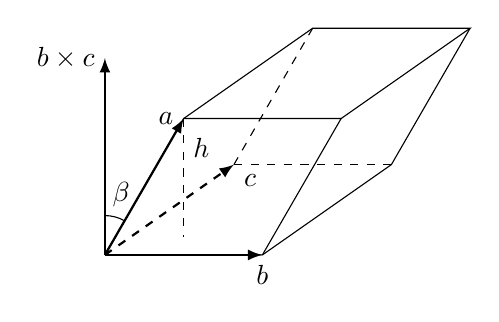
\begin{tikzpicture}
\pgfmathsetmacro{\kx}{2}
\pgfmathsetmacro{\ky}{2}
\pgfmathsetmacro{\kz}{2}
\pgfmathsetmacro{\angB}{60}
\pgfmathsetmacro{\angA}{35}
%parallelopiped visible
\draw(0,0)--++(\ky,0)--++(\angB:\kz)--++(-\ky,0)coordinate(UL)--++(\angB:-\kz);
\draw(UL)--++(\angA:\kx)--++(\ky,0)coordinate(BRT)--++(\angA:-\kx);
\draw(BRT)--++(\angB:-\kz)--++(\angA:-\kx);
%invisible
\draw[-latex,dashed,thick](0,0)--++(\angA:\kx)node[below right]{$\bM{c}$};
\draw[dashed](0,0)++(\angA:\kx)--++(\angB:\kz);
\draw[dashed](0,0)++(\angA:\kx)--++(\ky,0);
%sides
\draw[-latex,thick](0,0)--++(\ky,0)node[below]{$\bM{b}$};
\draw[-latex,thick](0,0)--++(\angB:\kz)node[left]{$\bM{a}$};
%text
\draw[-latex,thick](0,0)--++(0,2.5)node[left]{$\bM{b}\times \bM{c}$};
\draw[dashed](0,0)++(\angB:\kz)--++(0,-3/4*\kz)node[pos=0.25,right]{$h$};
\draw([shift={(\angB:0.5)}]0,0) arc (\angB:90:0.5);
\draw(75:0.8)node{$\beta$};
\end{tikzpicture}
\caption{غیر سمتی سہ ضرب کی جیومیٹریائی معنی۔}
\label{شکل_الجبرا_غیر_سمتی_سہ_ضرب}
\end{figure}

ہم نے دیکھا کہ غیر سمتی سہ ضرب در حقیقت متوازی شش پہلو کا حجم دیتا ہے۔اب کسی چیز کا حجم ایک مستقل ہے جو چنے گئے دائیں ہاتھ کارتیسی نظام پر منحصر نہیں ہو گا لہٰذا غیر سمتی سہ ضرب کا دارومدار بھی زیر استعمال دائیں ہاتھ کارتیسی  نظام پر نہیں ہو گا۔البتہ یاد رہے کہ بائیں ہاتھ کارتیسی نظام کی صورت میں مساوات \حوالہ{مساوات_الجبرا_سمتی_ضرب_مقطع_ب} کی جگہ مساوات \حوالہ{مساوات_الجبرا_سمتی_ضرب_مقطع_پ} استعمال ہو گا جس سے مساوات \حوالہ{مساوات_الجبرا_غیر_سمتی_سہ_ضرب_الف} میں مقطع کے سامنے \عددی{-1} نمودار ہو گا۔ہم یہ بھی کہہ سکتے ہیں کہ مقطع کی قیمت ایک دائیں ہاتھ نظام کی جگہ دوسرا دائیں ہاتھ کا نظام استعمال کرنے سے تبدیل نہیں ہو گا اور نا ہی یہ ایک بائیں ہاتھ نظام کی جگہ دوسرا بائیں ہاتھ نظام استعمال کرنے سے تبدیل ہو گا البتہ دائیں ہاتھ نظام کی جگہ بائیں ہاتھ نظام یا بائیں ہاتھ نظام کی جگہ دائیں ہاتھ نظام استعمال کرنے سے مقطع کی قیمت \عددی{-1} سے ضرب ہو گی۔  
%=====================
\ابتدا{مثال}\شناخت{مثال_الجبرا_چو_سطحہ}\quad چو سطحہ\\
دائیں ہاتھ کارتیسی نظام میں چو سطحہ کے قریبی اطراف درج ذیل ہیں۔اس چو سطحہ کا حجم دریافت کریں (شکل \حوالہ{شکل_مثال_الجبرا_چو_سطحہ})۔
\begin{align*}
\bM{a}=\bM{i}+\bM{j},\quad \bM{b}=2\bM{i}+3\bM{j}+4\bM{k},\quad \bM{c}=3\bM{i}+5\bM{j}+2\bM{k}
\end{align*}
حل:متوازی شش پہلو کا حجم درج ذیل مقطع سے حاصل ہو گا۔
\begin{align*}
\begin{vmatrix}1&1&0\\2&3&4\\3&5&2  \end{vmatrix}=-6
\end{align*}
یوں متوازی شش پہلو کا حجم \عددی{V=6} ہے۔مقطع کی قیمت منفی ہے جس کا مطلب ہے کہ \عددی{\bM{a}}، \عددی{\bM{b}}، \عددی{\bM{c}} سمتیات اسی ترتیب میں بائیں ہاتھ ثلاثہ سمتیات ہیں۔چو سطحہ کا حجم متوازی شش پہلو کے حجم کا \عددی{\tfrac{1}{8}} ہے لہٰذا اس کا حجم \عددی{\tfrac{3}{4}} ہو گا۔
\begin{figure}
\centering
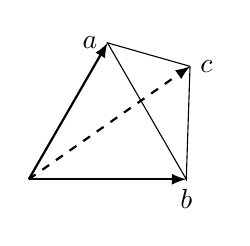
\begin{tikzpicture}
\pgfmathsetmacro{\kx}{2.5}
\pgfmathsetmacro{\ky}{2}
\pgfmathsetmacro{\kz}{2}
\pgfmathsetmacro{\angB}{60}
\pgfmathsetmacro{\angA}{35}
%
\draw[-latex,dashed,thick](0,0)--++(\angA:\kx)node[right]{$\bM{c}$}coordinate(kkA);
%sides
\draw[-latex,thick](0,0)--++(\ky,0)node[below]{$\bM{b}$}coordinate(kkB);
\draw[-latex,thick](0,0)--++(\angB:\kz)node[left]{$\bM{a}$}coordinate(kkC);
\draw(kkA)--(kkB)--(kkC)--(kkA);
\end{tikzpicture}
\caption{غیر سمتی سہ ضرب سے چو سطحہ کے حجم کا حصول (مثال \حوالہ{مثال_الجبرا_چو_سطحہ})۔}
\label{شکل_مثال_الجبرا_چو_سطحہ}
\end{figure}

\انتہا{مثال}
%=========================
غیر سمتی سہ ضرب کی جیومیٹریائی معنی سے ہمیں تین سمتیات کی خطی طور تابعیت اور غیر تابعیت کا اصول بھی ملتا ہے۔یہ سمتیات صرف اور صرف ہم سطحی ہونے کی صورت میں خطی طور تابع ہوں گے [جس میں (حصہ \حوالہ{حصہ_الجبرا_سمتیات_فضا_تابعیت} میں دیا گیا) خطی طور تابع تین سمتیات کے ہم خطی ہونے کا شرط بھی شامل ہے]۔
%=====================

\ابتدا{مسئلہ}\شناخت{مسئلہ_الجبرا_تابعیت_غیر_سمتی_سہ_ضرب}\quad خطی تابعیت\\
تین سمتیات صرف اور صرف اس صورت خطی طور تابع ہوں گے جب ان کا غیر سمتی سہ ضرب صفر کے برابر ہو گا۔
\انتہا{مسئلہ}
%=========================

عملی استعمال میں درپیش دیگر متعدد ضرب کو نقطہ ضرب، صلیبی ضرب اور غیر سمتی سہ ضرب کی صورت میں لکھا جا سکتا ہے۔ایسا کرنے میں درج ذیل کلیہ (جس کا ثبوت جلد پیش کیا جائے گا) اہم کردار ادا کرتا ہے
\begin{align}\label{مساوات_الجبرا_خطیت_اور_حجم_الف}
\bM{b}\times (\bM{c}\times \bM{d})=(\bM{b}\cdot \bM{d})\bM{c}-(\bM{b}\cdot\bM{c})\bM{d}
\end{align}
جس سے مراد درج ذیل \اصطلاح{لیگرینج مماثل}\فرہنگ{لیگرینج!مماثل}\فرہنگ{مماثل!لیگرینج}\حاشیہب{Lagrange's identity}\فرہنگ{Lagrange!identity} 
\begin{align}\label{مساوات_الجبرا_خطیت_اور_حجم_ب}
(\bM{a}\times \bM{b})\cdot(\bM{c}\times\bM{d})=(\bM{a}\cdot\bM{c})(\bM{b}\cdot\bM{d})-(\bM{a}\cdot\bM{d})(\bM{b}\cdot\bM{c})
\end{align}
اور
\begin{align}\label{مساوات_الجبرا_خطیت_اور_حجم_پ}
(\bM{a}\times \bM{b})\times(\bM{c}\times\bM{d})=(\bM{a}\,\bM{b}\,\bM{d})\bM{c}-(\bM{a}\,\bM{b}\,\bM{c})\bM{d}
\end{align}
ہے، جن کے ثبوت آپ سے بالترتیب سوال \حوالہ{سوال_مساوات_الجبرا_خطیت_اور_حجم_ب} اور سوال \حوالہ{سوال_مساوات_الجبرا_خطیت_اور_حجم_پ} میں مانگے گئے ہیں۔مساوات \حوالہ{مساوات_الجبرا_خطیت_اور_حجم_الف}  کے ثبوت سے پہلے ہم دیکھتے ہیں کہ مساوات \حوالہ{مساوات_الجبرا_خطیت_اور_حجم_الف} سے مراد درج ذیل بھی ہے۔
\begin{align*}
(\bM{b}\times \bM{c})\times \bM{d}=-\bM{d}\times (\bM{b}\times \bM{c})=(\bM{d}\cdot \bM{b})\bM{c}-(\bM{d}\cdot\bM{c})\bM{b}
\end{align*}
اس سے ظاہر ہے کہ عموماً \عددی{\bM{b}\times (\bM{c}\times \bM{d})} اور \عددی{(\bM{b}\times \bM{c})\times \bM{d}} مختلف ہوں گے یعنی سمتی ضرب،  قانون تلازم پر پورا نہیں اترتا لہٰذا مساوات \حوالہ{مساوات_الجبرا_خطیت_اور_حجم_الف} میں قوسین لکھنا لازمی ہے اور انہیں ہٹایا نہیں جا سکتا ہے۔مثال کے طور پر دائیں ہاتھ کے نظام میں درج ذیل ہو گا۔
\begin{align*}
(\bM{i}\times \bM{j})\times \bM{j}=\bM{k}\times \bM{j}=-\bM{i} \quad \text{لیکن}\quad \quad \bM{i}\times (\bM{j}\times \bM{j})=\bM{0}
\end{align*}
%==========================
\ابتدا{ثبوت}\quad برائے مساوات \حوالہ{مساوات_الجبرا_خطیت_اور_حجم_الف}\\
ہم دائیں ہاتھ کارتیسی محدد یوں چنتے ہیں کہ \عددی{x} محور کی سمت \عددی{\bM{d}} ہو اور \عددی{xy} سطح میں \عددی{\bM{c}} پایا جاتا ہو۔یوں مساوات \حوالہ{مساوات_الجبرا_خطیت_اور_حجم_الف} کے سمتیات درج ذیل لکھے جائیں گے
\begin{align*}
\bM{b}=b_1\bM{i}+b_2\bM{j}+b_3\bM{k},\quad \bM{c}=c_1\bM{i}+c_2\bM{j},\quad \bM{d}=d_1\bM{i}
\end{align*}
لہٰذا \عددی{\bM{c}\times \bM{d}=-c_2d_1\bM{k}} ہو گا جس کو استعمال کرتے ہوئے درج ذیل لکھا جا سکتا ہے۔
\begin{align*}
\bM{b}\times (\bM{c}\times \bM{d})=\begin{vmatrix}\bM{i}&\bM{j}&\bM{k}\\b_1&b_2&b_3\\0&0&-c_2d_1  \end{vmatrix}=-b_2c_2d_1\bM{i}+b_1c_2d_1\bM{j}
\end{align*} 
ساتھ ہی ساتھ ہم درج ذیل بھی لکھ سکتے ہیں۔
\begin{align*}
(\bM{b}\cdot\bM{d})\bM{c}-(\bM{b}\cdot\bM{c})\bM{d}=b_1d_1(c_1\bM{i}+c_2\bM{j})-(b_1c_1+b_2c_2)d_1\bM{i}=b_1c_2d_1\bM{j}-b_2c_2d_1\bM{i}
\end{align*}
یوں ہماری مخصوص کارتیسی نظام میں مساوات \حوالہ{مساوات_الجبرا_خطیت_اور_حجم_الف} ثابت ہوتا ہے۔اب سمتیہ کی لمبائی، سمتیہ  کا رخ، سمتی ضرب اور غیر سمتی ضرب کی قیمت کا دارومدار چنے گئے نظام پر ہرگز نہیں ہوتا۔ مزید دہرا سمتی ضرب کی بنا \عددی{\bM{b}\times (\bM{c}\times \bM{d})} کو دائیں ہاتھ یا بائیں ہاتھ کارتیسی نظام میں \عددی{\bM{i}}، \عددی{\bM{j}}، \عددی{\bM{k}}  کی صورت میں لکھنے سے یکساں جواب ملتا ہے۔یوں مساوات \حوالہ{مساوات_الجبرا_خطیت_اور_حجم_الف} کسی بھی کارتیسی نظام کے لئے درست ہے۔
\انتہا{ثبوت}

%========================
\حصہء{سوالات}
سوال \حوالہ{سوال_الجبرا_غیر-سمتی_سہ_ضرب_الف} تا سوال \حوالہ{سوال_الجبرا_غیر-سمتی_سہ_ضرب_ب} میں دائیں ہاتھ کارتیسی نظام استعمال کیا گیا ہے۔ان سوالات میں دیے گئے تین سمتیات کا غیر سمتی سہ ضرب \عددی{\bM{a}\cdot(\bM{b}\times \bM{c})} دریافت کریں۔

%===============
\ابتدا{سوال}\شناخت{سوال_الجبرا_غیر-سمتی_سہ_ضرب_الف}\quad
$\bM{a}=\bM{i},\,\bM{b}=\bM{j},\,\bM{c}=\bM{k}$\\
جواب:\عددی{1}
\انتہا{سوال}
%=====================
\ابتدا{سوال}\quad
$\bM{a}=\bM{j},\,\bM{b}=\bM{k},\,\bM{c}=\bM{i}$\\
جواب:\عددی{1}
\انتہا{سوال}
%=====================
\ابتدا{سوال}\quad
$\bM{a}=\bM{i},\,\bM{b}=\bM{k},\,\bM{c}=\bM{j}$\\
جواب:\عددی{-1}
\انتہا{سوال}
%=====================
\ابتدا{سوال}\quad
$\bM{a}=3\bM{i},\,\bM{b}=\bM{j}-\bM{k},\,\bM{c}=4\bM{j}+3\bM{k}$\\
جواب:\عددی{28}
\انتہا{سوال}
%=====================
\ابتدا{سوال}\quad
$\bM{a}=5\bM{j},\,\bM{b}=\bM{j}+\bM{k},\,\bM{c}=2\bM{i}+3\bM{k}$\\
جواب:\عددی{10}
\انتہا{سوال}
%=====================
\ابتدا{سوال}\quad
$\bM{a}=\bM{i}-2\bM{j}+3\bM{k},\,\bM{b}=-\bM{i}+\bM{j}+3\bM{k},\,\bM{c}=2\bM{i}-3\bM{j}+3\bM{k}$\\
جواب:\عددی{-3}
\انتہا{سوال}
%=====================
\ابتدا{سوال}\quad
$\bM{a}=2\bM{i}+\bM{k},\,\bM{b}=-\bM{i}+\bM{j},\,\bM{c}=3\bM{j}+2\bM{k}$\\
جواب:\عددی{1}
\انتہا{سوال}
%=====================
\ابتدا{سوال}\quad
$\bM{a}=2\bM{i}-4\bM{j}+\bM{k},\,\bM{b}=\bM{j},\,\bM{c}=2\bM{i}-5\bM{j}+7\bM{k}$\\
جواب:\عددی{12}
\انتہا{سوال}
%=====================
\ابتدا{سوال}\quad
$\bM{a}=\bM{i}+4\bM{j}-\bM{k},\,\bM{b}=-\bM{i},\,\bM{c}=-2\bM{i}+7\bM{j}+3\bM{k}$\\
جواب:\عددی{19}
\انتہا{سوال}
%=====================
\ابتدا{سوال}\شناخت{سوال_الجبرا_غیر-سمتی_سہ_ضرب_ب}\quad
$\bM{a}=5\bM{i}-\bM{j}-\bM{k},\,\bM{b}=\bM{k},\,\bM{c}=7\bM{j}+3\bM{k}$\\
جواب:\عددی{-35}
\انتہا{سوال}
%=====================
کیا سوال \حوالہ{سوال_الجبرا_تابع_غیر_تابع_الف} تا سوال \حوالہ{سوال_الجبرا_تابع_غیر_تابع_ب} کے سمتیات خطی طور تابع یا خطی طور غیر تابع ہیں؟ 

%==============
\ابتدا{سوال}\شناخت{سوال_الجبرا_تابع_غیر_تابع_الف}\quad
$\bM{i},\, \bM{j}$\\
جواب: غیر تابع
\انتہا{سوال}
%=====================
\ابتدا{سوال}\quad
$\bM{i}-6\bM{j}+2\bM{k},\, 2\bM{j}+7\bM{k},\, -2\bM{i}+12\bM{j}-4\bM{k}$\\
جواب: تابع
\انتہا{سوال}
%=====================
\ابتدا{سوال}\quad
$2\bM{i}+6\bM{j}-2\bM{k},\, 2\bM{j}+3\bM{k},\, -2\bM{i}+2\bM{j}-\bM{k}$\\
جواب: غیر تابع
\انتہا{سوال}
%=====================
\ابتدا{سوال}\quad
$-3\bM{i}+6\bM{j}+2\bM{k},\, 4\bM{i}+3\bM{j},\, 2\bM{i}-2\bM{j}+\bM{k}$\\
جواب: غیر تابع
\انتہا{سوال}
%=====================
\ابتدا{سوال}\quad
$4\bM{i}+5\bM{j},\, \bM{i}+2\bM{j},\, -\bM{i}+3\bM{j}$\\
جواب: تابع
\انتہا{سوال}
%=====================
\ابتدا{سوال}\quad
$\bM{i}+\bM{k},\, 3\bM{i}-5\bM{k},\, 8\bM{k}$\\
جواب: تابع
\انتہا{سوال}
%=====================
\ابتدا{سوال}\quad
$\bM{i}+\bM{j},\, 3\bM{i}-5\bM{k},\, 2\bM{i}$\\
جواب: غیر تابع
\انتہا{سوال}
%=====================
\ابتدا{سوال}\شناخت{سوال_الجبرا_تابع_غیر_تابع_ب}\quad
$\bM{j}-\bM{k},\, \bM{i}-\bM{k},\, \bM{j}$\\
جواب: غیر تابع
\انتہا{سوال}
%=====================
\ابتدا{سوال}\quad
\عددی{\lambda} کی وہ قیمت دریافت کریں جس سے درج ذیل تینوں سمتیات ہم خطی ہوں گے۔\\
$\bM{i}+6\bM{j}-8\bM{k},\, 2\bM{i}-\bM{j}-\bM{k},\, \lambda\bM{i}+\bM{j}+\bM{k}$\\
جواب:\عددی{\lambda=-2}
\انتہا{سوال}
%=====================
\ابتدا{سوال}
کیا درج ذیل چار نقطے ہم سطحی ہیں؟
\begin{align*}
(4,-2,1),\,(5,1,6),\,(2,2,-5),\,(3,5,0)
\end{align*}
جواب:غیر ہم سطحی
\انتہا{سوال}
%======================
\ابتدا{سوال}
درج ذیل میں \عددی{\alpha} اور \عددی{\beta} کی وہ قیمتیں دریافت کریں جو تینوں نقطوں کو ہم خطی بناتے ہیں۔
\begin{align*}
(-1,3,2),\, (-4,2,-2),\, (5,\alpha,\beta)
\end{align*}
جوابات:\عددی{\alpha=5}، \عددی{\beta=10}
\انتہا{سوال}
%========================
\ابتدا{سوال}
تین متغیرات پر مبنی تین مساوات کی متجانس نظام کا غیر صفر حل صرف اور صرف اس صورت ممکن ہو گا جب نظام کی عددی سر قالب کا مقطع صفر ہو۔اس حقیقت کو استعمال کرتے ہوئے مسئلہ \حوالہ{مسئلہ_الجبرا_تابعیت_غیر_سمتی_سہ_ضرب} ثابت کریں۔ 
\انتہا{سوال}
%========================
سوال \حوالہ{سوال_الجبرا_متوازی_شہ_پہلو_الف} تا سوال \حوالہ{سوال_الجبرا_متوازی_شہ_پہلو_ب} میں متوازی شہ پہلو کے قریبی اطراف دیے گئے ہیں۔ متوازی شہ پہلو کا حجم دریافت کریں۔

%==============
\ابتدا{سوال}\شناخت{سوال_الجبرا_متوازی_شہ_پہلو_الف}\quad
$\bM{i},\, \bM{j},\,-\bM{k}$\\
جواب:\عددی{1}
\انتہا{سوال}
%==================
\ابتدا{سوال}\quad
$\bM{i}-\bM{j},\, \bM{j}-\bM{k},\,\bM{i}+\bM{k}$\\
جواب:\عددی{2}
\انتہا{سوال}
%==================
\ابتدا{سوال}\quad
$2\bM{i}+\bM{j}+3\bM{k},\, \bM{i}+\bM{j}-\bM{k},\,\bM{i}-2\bM{j}+\bM{k}$\\
جواب:\عددی{13}
\انتہا{سوال}
%==================
\ابتدا{سوال}\quad
$3\bM{i}-2\bM{j}+3\bM{k},\, \bM{i}-2\bM{j}-3\bM{k},\,\bM{i}-4\bM{j}+\bM{k}$\\
جواب:\عددی{40}
\انتہا{سوال}
%==================
\ابتدا{سوال}\quad
$3\bM{i}+2\bM{j}+3\bM{k},\, \bM{i}+2\bM{j}+3\bM{k},\,\bM{i}+4\bM{j}+\bM{k}$\\
جواب:\عددی{20}
\انتہا{سوال}
%==================
\ابتدا{سوال}\شناخت{سوال_الجبرا_متوازی_شہ_پہلو_ب}\quad
$3\bM{i}+3\bM{j}+4\bM{k},\, 2\bM{i}+3\bM{j}+\bM{k},\,\bM{i}+3\bM{j}+2\bM{k}$\\
جواب:\عددی{12}
\انتہا{سوال}
%==================
سوال \حوالہ{سوال_الجبرا_چو_سطحہ_الف} تا سوال \حوالہ{سوال_الجبرا_چو_سطحہ_ب} میں چو سطحہ کے کونے دیے گئے ہیں۔اس کا حجم دریافت کریں۔

%============
\ابتدا{سوال}\شناخت{سوال_الجبرا_چو_سطحہ_الف}\quad
$(0,0,0),\,(2,4,0),\,(0,2,4),\,(3,5,6)$\\
جواب:\عددی{4}
\انتہا{سوال}
%=====================
\ابتدا{سوال}\quad
$(3,4,2),\,(1,-2,3),\,(2,2,2),\,(6,3,5)$\\
جواب:\عددی{\tfrac{1}{8}}
\انتہا{سوال}
%=====================
\ابتدا{سوال}\quad
$(0,0,0),\,(1,0,0),\,(0,1,0),\,(0,0,1)$\\
جواب:\عددی{\tfrac{1}{8}}
\انتہا{سوال}
%=====================
\ابتدا{سوال}\شناخت{سوال_الجبرا_چو_سطحہ_ب}\quad
$(-3,2,-1),\,(1,2,5),\,(-2,1,3),\,(4,-1,1)$\\
جواب:\عددی{8}
\انتہا{سوال}
%=====================
سوال \حوالہ{سوال_الجبرا_دیگر_متعدد_ضرب_الف} تا سوال \حوالہ{سوال_الجبرا_دیگر_متعدد_ضرب_ب} میں \عددی{\bM{a}=2\bM{i}-\bM{j}+3\bM{k}}، \عددی{\bM{b}=\bM{i}+2\bM{j}+2\bM{k}}، \عددی{\bM{c}=-3\bM{i}-4\bM{j}+5\bM{k}} اور \عددی{\bM{d}=4\bM{i}+\bM{j}-\bM{k}} لیں۔

%=================
\ابتدا{سوال}\شناخت{سوال_الجبرا_دیگر_متعدد_ضرب_الف}\quad
$(\bM{a}\times \bM{b})\times \bM{c},\, \bM{a}\times (\bM{b}\times \bM{c})$\\
جوابات:
$(\bM{a}\times \bM{b})\times \bM{c}=15\bM{i}+25\bM{j}+29\bM{k},\,\bM{a}\times (\bM{b}\times \bM{c})=31\bM{i}+50\bM{j}-4\bM{k} $
\انتہا{سوال}
%====================
\ابتدا{سوال}\quad
$(\bM{b}\times \bM{c})\times \bM{d},\, \bM{d}\times (\bM{b}\times \bM{c})$\\
جوابات:
$(\bM{b}\times \bM{c})\times \bM{d}=9\bM{i}+26\bM{j}+62\bM{k},\,\bM{d}\times (\bM{b}\times \bM{c})=-9\bM{i}-26\bM{j}-64\bM{k} $
\انتہا{سوال}
%====================
\ابتدا{سوال}\quad
$(\bM{a}\times \bM{c})\times \bM{d},\, \bM{a}\times (\bM{d}\times \bM{c})$\\
جوابات:
$(\bM{a}\times \bM{c})\times \bM{d}=30\bM{i}-37\bM{j}+83\bM{k},\,\bM{a}\times (\bM{d}\times \bM{c})=64\bM{i}+29\bM{j}-33\bM{k} $
\انتہا{سوال}
%====================
\ابتدا{سوال}\quad
$(\bM{a}\times \bM{a})\times \bM{d},\, \bM{a}\times (\bM{a}\times \bM{d})$\\
جوابات:
$(\bM{a}\times \bM{a})\times \bM{d}=\bM{0},\,\bM{a}\times (\bM{a}\times \bM{d})=-48\bM{i}-18\bM{j}+26\bM{k} $
\انتہا{سوال}
%====================
\ابتدا{سوال}\quad
$(\bM{a}\times \bM{b})\times (\bM{c}\times \bM{d})$\\
جوابات:
$-98\bM{i}+99\bM{j}-137\bM{k} $
\انتہا{سوال}
%====================
\ابتدا{سوال}\شناخت{سوال_الجبرا_دیگر_متعدد_ضرب_ب}\quad
$(\bM{a}\times \bM{b})\cdot(\bM{c}\times \bM{d})\cdot (\bM{c}\times \bM{a})\cdot(\bM{d}\times \bM{b})$\\
جوابات:
$-6832$
\انتہا{سوال}
%====================
\ابتدا{سوال}\شناخت{سوال_مساوات_الجبرا_خطیت_اور_حجم_ب}
مساوات \حوالہ{مساوات_الجبرا_خطیت_اور_حجم_ب} ثابت کریں۔
\انتہا{سوال}
%======================
\ابتدا{سوال}\شناخت{سوال_مساوات_الجبرا_خطیت_اور_حجم_پ}
مساوات \حوالہ{مساوات_الجبرا_خطیت_اور_حجم_پ} ثابت کریں۔
\انتہا{سوال}
%======================
